\documentclass[10pt,landscape]{article}
\usepackage{amssymb,amsmath,amsthm,amsfonts}
\usepackage{multicol,multirow}
\usepackage{calc}
\usepackage{ifthen}
\usepackage{graphicx}
\usepackage{xcolor}
\usepackage[utf8]{inputenc}
\usepackage{cprotect}
\usepackage{enumitem}
\usepackage{listings} 
\usepackage[landscape]{geometry}
\usepackage[colorlinks=true,citecolor=blue,linkcolor=blue]{hyperref}
\usepackage{fancyhdr}
\usepackage{ragged2e}
\usepackage{ulem}


\lstset{
    tabsize=2,    
%   rulecolor=,
    language={C},
        captionpos = t,
        basicstyle = \scriptsize\ttfamily,
        frame=lines,
        numbersep=5pt,
        numbers=left,
        numberstyle=\scriptsize,
        backgroundcolor=\color{white},
        columns=fixed,
        extendedchars=false,
        breaklines=true,
        prebreak = \raisebox{0ex}[0ex][0ex]{\ensuremath{\hookleftarrow}},
        frame=single,
        showtabs=false,
        showspaces=false,
        showstringspaces=false,
        keywordstyle=\color[rgb]{0,0,1},
        keywordstyle=[2]\color{gray},
        commentstyle=\color{teal},
        stringstyle=\color{red},
        numberstyle=\color[rgb]{0.205, 0.142, 0.73},
}

\ifthenelse{\lengthtest { \paperwidth = 11in}}
    { \geometry{top=.25in,left=.25in,right=.25in,bottom=.25in} }
	{\ifthenelse{ \lengthtest{ \paperwidth = 297mm}}
		{\geometry{top=1cm,left=1cm,right=1cm,bottom=1cm} }
		{\geometry{top=1cm,left=1cm,right=1cm,bottom=1cm} }
	}
\pagestyle{empty}
\makeatletter
\renewcommand{\subsection}{\@startsection{section}{1}{0mm}%
                                {-1ex plus -.5ex minus -.2ex}%
                                {0.5ex plus .2ex}%x
                                {\normalfont\large\bfseries}}
\renewcommand{\subsection}{\@startsection{subsection}{2}{0mm}%
                                {-1explus -.5ex minus -.2ex}%
                                {0.5ex plus .2ex}%
                                {\normalfont\normalsize\bfseries}}
\renewcommand{\subsubsection}{\@startsection{subsubsection}{3}{0mm}%
                                {-1ex plus -.5ex minus -.2ex}%
                                {1ex plus .2ex}%
                                {\normalfont\small\bfseries}}
\makeatother
\setcounter{secnumdepth}{0}
\setlength{\parindent}{0pt}
\setlength{\parskip}{0pt plus 0.5ex}

\title{CS2106-cheatsheet}
% -----------------------------------------------------------------------

\begin{document}

\raggedright
\footnotesize


\begin{multicols*}{3}
    \begin{tiny}
        \small{\textbf{CS2106 Cheatsheet AY22/23 || \href{https://github.com/JasonYapzx}{@JasonYapzx}}} \\
   \end{tiny}
\setlength{\premulticols}{1pt}
\setlength{\postmulticols}{1pt}
\setlength{\multicolsep}{1pt}
\setlength{\columnsep}{2pt}

\subsection*{Motivation for OS}
\begin{itemize}[topsep=0pt,noitemsep,wide=0pt, leftmargin=\dimexpr\labelwidth + 2\labelsep\relax, topsep=0pt]
    \item Abstraction $\rightarrow$\ ease of programming, portability, efficiency
    \item Resource Allocator $\rightarrow$\ asynchronous programs running
    \item Control Program $\rightarrow$\ prevents errors, provides security
\end{itemize}

\subsection*{\underline{OS Components}}
Operating systems are essentially software, where they run in \textit{kernel mode}, giving \underline{full access} to all hardware resources. Other software usually executes in \textit{user mode} with limited access to hardware resources. \\

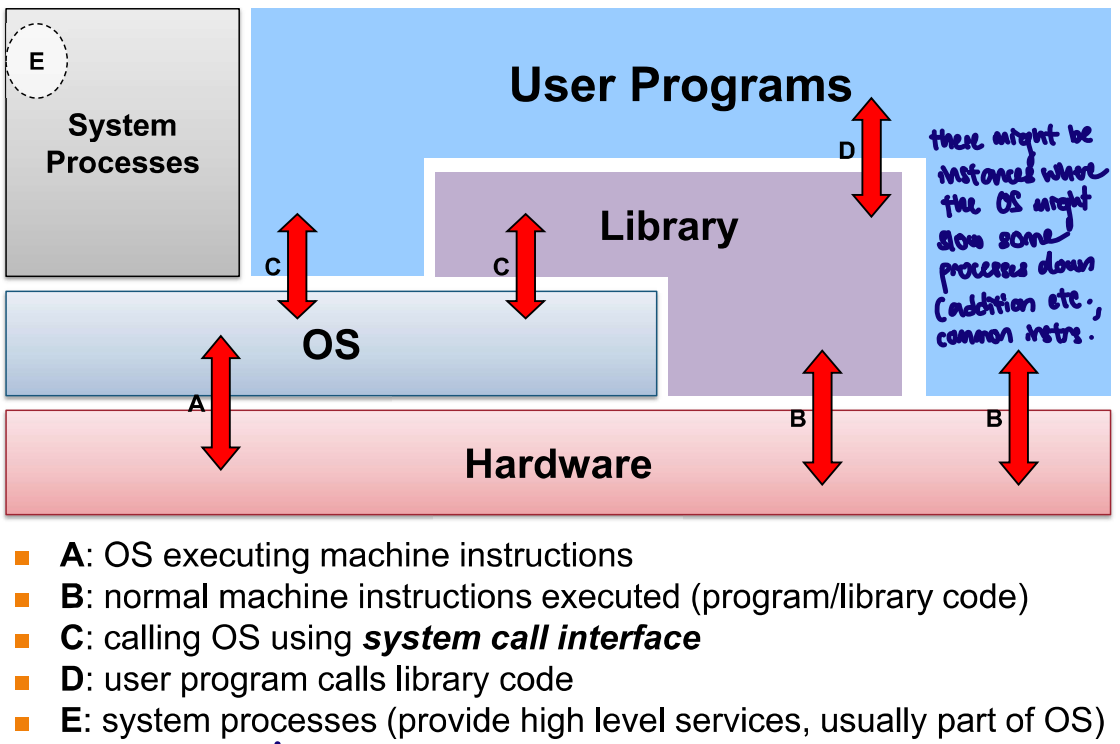
\includegraphics[scale=0.4]{images/generic_os.png}

\subsection*{OS Structures}
\subsubsection*{Monolithic OS}
Monolithic as the name suggests, has \underline{ONE BIG} program as its OS, where all its process, memory, file system and system call interface are within the same program.

$\bullet$\ Advantages: well understand \& great performance

$\bullet$\ Disadvantages: highly coupled, complicated internal structure
\subsubsection*{Microkernel OS}
Kernel is small and clean, and only provides the basic and essential facilities. The higher level services are built on top of the basic facilities.

$\bullet$\ Advantages: kernel is more modular + robust $\rightarrow$\ easily extendible, good isolation between kernel / high-level services.

$\bullet$\ Disadvantages: less performance

\subsection*{Virtual Machines / Hypervisors}
Software emulation of hardware (\textbf{virtualization}).
\begin{itemize}[topsep=0pt,noitemsep,wide=0pt, leftmargin=\dimexpr\labelwidth + 2\labelsep\relax, topsep=0pt]
    \item \textbf{Type 1 hypervisor OS:} provides individual \textbf{virtual machines} to guest OSes $\rightarrow$\ similar to on-premise hosting of different OSes, cloud providers giving resources for people to run containers/servers.
    \item \textbf{Type 2 hypervisor OS:} Runs in the host OS guest OS runs inside Virtual Machine $\rightarrow$\ similar to VirtualBox emulation, it uses resources as part of a program to emulate the virtual OS.
\end{itemize}


\subsection*{\underline{Process Abstraction}}

\subsection*{Components}
    \begin{itemize}[topsep=0pt,noitemsep,wide=0pt, leftmargin=\dimexpr\labelwidth + 2\labelsep\relax, topsep=0pt]
        \item \underline{Memory context:} Text, Data, \textbf{Stack} and \textbf{Heap}
        \item \underline{Hardware context:} \textbf{General Purpose Registers (GPR)}, PC, Stack/Frame Pointer (SP/FP)
    \end{itemize}
\subsection*{Control Flow and Data}
\textbf{\underline{Stack Memory Region:}} where information and function invocation is stored. \underline{Stack Pointer} points
to the top of stack region (first free location). Information needed for function
invocation is described as a \underline{stack frame} and contains: \vspace*{2pt}
\begin{multicols*}{2}
    \begin{itemize}[topsep=0pt,noitemsep,wide=0pt, leftmargin=\dimexpr\labelwidth + 2\labelsep\relax]
        \item return address of caller
        \item arguments (params) 
        \item local variable storage
        \item \textbf{common additional information}: frame pointer/saved registers
    \end{itemize}
\end{multicols*} \vspace*{2pt}

\textbf{\underline{Frame pointer:}} facilitates access of various stack frame items, points to a \textit{}{fixed location} in the stack frame.
\\ \textbf{\underline{Saved Registers:}} prevent \textit{register spilling}, GPRs are usually limited on processers. Functions spill registers
it intends to use before starting, restoring them at the \textit{end of the function}.
\subsubsection*{Stack Frame Setup / Teardown}
\textit{On executing function call}:
\begin{itemize}[topsep=0pt,noitemsep,wide=0pt, leftmargin=\dimexpr\labelwidth + 2\labelsep\relax]
    \item \colorbox{orange!80}{% 
        \textbf{Caller:} Pass arguments with registers and/or stack
    }
    \item \colorbox{orange!80}{% 
        \textbf{Caller:} Save Return PC on stack
    }
\end{itemize}
Transfer control from caller to callee:
\begin{itemize}[topsep=0pt,noitemsep,wide=0pt, leftmargin=\dimexpr\labelwidth + 2\labelsep\relax]
    \item \colorbox{teal!80}{%
        \textbf{Callee:} \underline{Save registers used by called.} Save old \underline{FP} and SP
    }
    \item \colorbox{teal!80}{%
        \textbf{Callee:} Allocated space for local variables of callee on stack
    }
    \item \colorbox{teal!80}{%
        \textbf{Callee:} Adjust SP to point to new stack top
    }
\end{itemize}
\textit{On returning from function call}:
\begin{itemize}[topsep=0pt,noitemsep,wide=0pt, leftmargin=\dimexpr\labelwidth + 2\labelsep\relax]
    \item \colorbox{teal!80}{%
        \textbf{Callee:} \underline{Restore saved registers}, \underline{FP} and SP
    }
\end{itemize}
Transfer control from callee to caller using saved PC:
\begin{itemize}[topsep=0pt,noitemsep,wide=0pt, leftmargin=\dimexpr\labelwidth + 2\labelsep\relax]
    \item \colorbox{orange!80}{%
        \textbf{Caller:} Continues execution in caller
    }
\end{itemize}
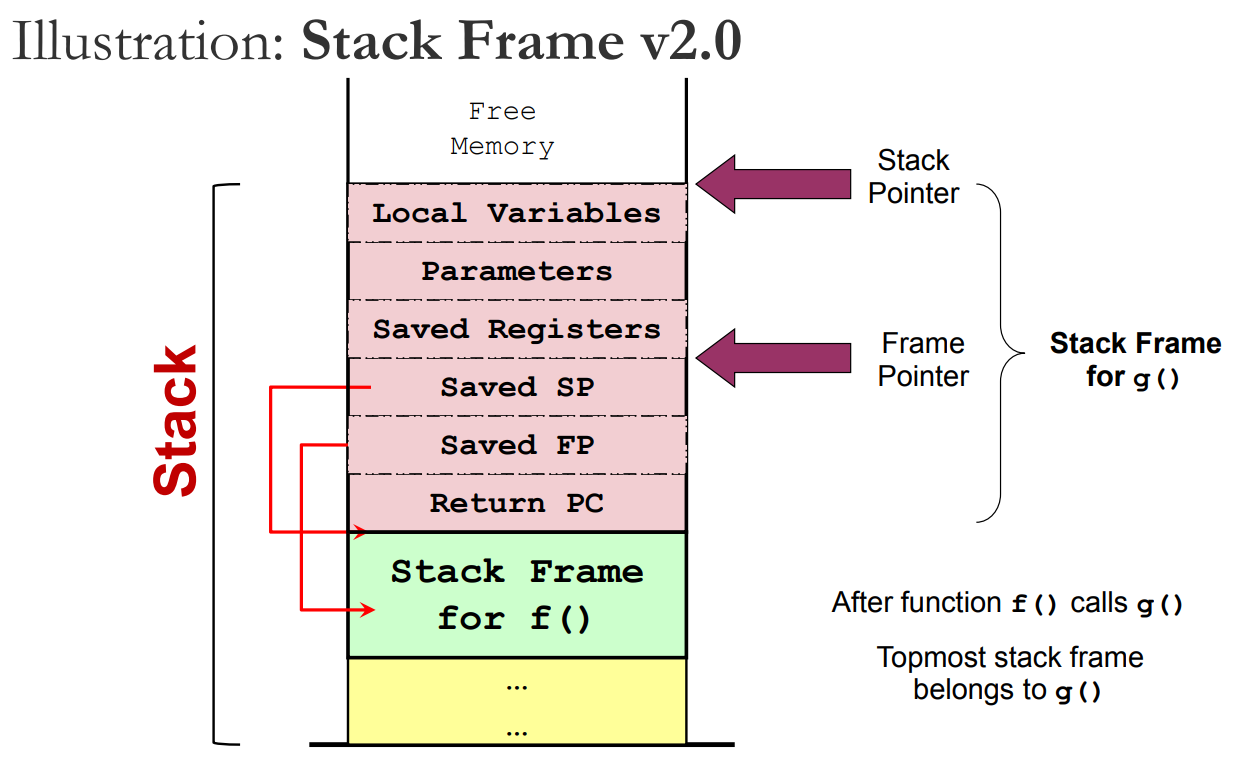
\includegraphics[scale=0.29]{images/stackframe.png}
\subsubsection*{Dynamicaly Allocated Memory}
\begin{itemize}[topsep=0pt,noitemsep,wide=0pt, leftmargin=\dimexpr\labelwidth + 2\labelsep\relax]
    \item Allocated only at runtime $\rightarrow$ size not known at compile time (cannot put int \verb|data| region)
    \item No definite deallocation timing $\rightarrow$ cannot be explicitly freed any time (cannot put int \verb|stack| region)
    \item Solution: setup a separate \textbf{heap memory region}
\end{itemize}

\subsection*{\underline{Processes}}
5-STAGE PROCESS MODEL (PROCESS State)
\begin{enumerate}[topsep=0pt,noitemsep,wide=0pt, leftmargin=\dimexpr\labelwidth + 2\labelsep\relax]
    \item \textbf{New:} process created / still initializing
    \item \textbf{Ready:} process waiting to run
    \item \textbf{Running:} process executed on CPU
    \item \textbf{Blocked:} waiting for event $\rightarrow$ $\times$ execute until event available
    \item \textbf{Terminated:} finished execution, may require OS cleanup
\end{enumerate}

\includegraphics*[width=8.5cm, height=3cm]{images/transitions.png}


\subsection*{Process Table}
Each process has a Process Control Block \textbf{PCB} (or Process Table Entry) that stores
the entire execution context for a process. These blocks are stored in the \textbf{Process Table} by the kernel.
\begin{itemize}[topsep=0pt,noitemsep,wide=0pt, leftmargin=\dimexpr\labelwidth + 2\labelsep\relax, topsep=0pt]
    \item HW Context: Only updated in PCB when process swapped out
    \item Mem Context: Not actual memory space used by the process
    \item OS Context: May contain information used for scheduling
\end{itemize}
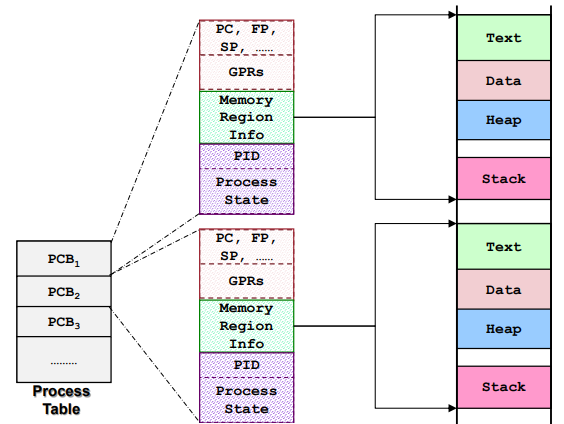
\includegraphics[height=3.3cm, width=4.2cm]{images/processtable.png}
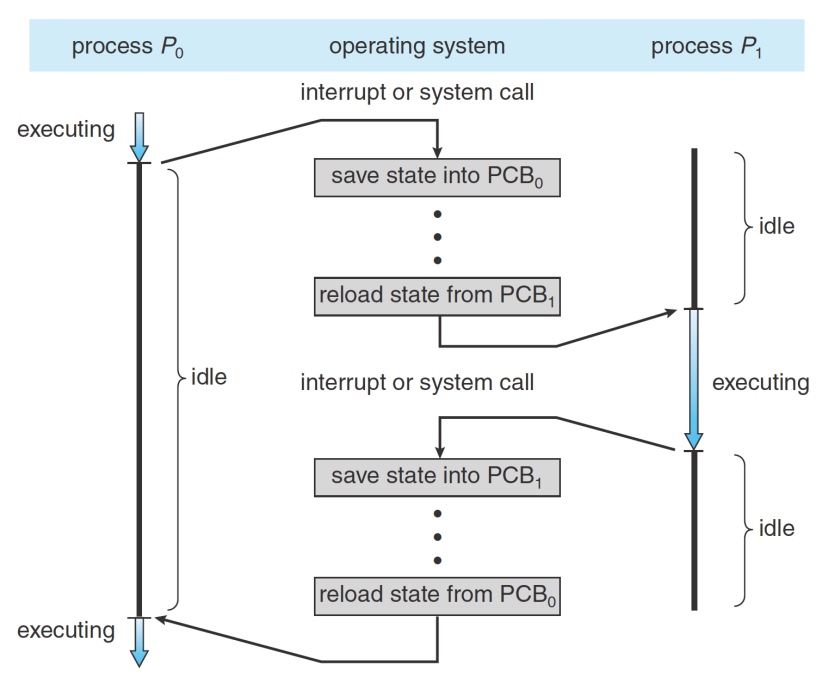
\includegraphics[height=3.3cm, width=4.2cm]{images/contextswitch.png}

\subsection*{\underline{Exceptions and Interrupts}}
Executing a \textbf{machine level instruction} can cause exceptions. They are \underline{synchronous}
and occur due to program execution. An \textbf{exception handler} is executed automatically,
similar to a forced function call. Examples: 
\begin{itemize}[topsep=0pt,noitemsep,wide=0pt, leftmargin=\dimexpr\labelwidth + 2\labelsep\relax]
    \item Arithmetic Errors: Overflow, Underflow, Division by zero
    \item Memory Errors: Illegal/Misaligned memory address
\end{itemize}

\subsection*{Interrupts}
\textbf{External events} that can interrupt the execution of a program. Intterupts are \underline{asynchronous}
and occur in events that are indepedent of program execution. The program exeuction is suspended,
and an \textbf{interrupt handler} is exeucted automatically.
\begin{itemize}[topsep=0pt,noitemsep,wide=0pt, leftmargin=\dimexpr\labelwidth + 2\labelsep\relax]
    \item Hardware related: Timer, mouse movement, keyboard press etc.
    \item Can be enabled/disabled (selectively or globally), prioritized, nested.
\end{itemize}

\subsubsection*{Interrupt Handling Steps: HW/SW Co-design}
The \underline{contract} between HW and SW around the IVT. OS populates IVT with address of interrupt routines.
HW reads the IVT automatically to locate the handler.

\begin{enumerate}[topsep=0pt,noitemsep,wide=0pt, leftmargin=\dimexpr\labelwidth + 2\labelsep\relax]
    \item PUSH (PC) -- hardware
    \item PUSH (status register) -- hardware
    \item Disable interrupts in the status register -- hardware
    \item Read \underline{Interrupt Vector Table (IVT)} entry number \#42 -- hardware
    $\rightarrow$ IVT a table where the OS stores the address of all interrupt handlers
    \item Switch to kernel mode -- hardware
    \item PC $\leftarrow$ \verb|handler_42()| -- hardware
    \item \verb|handler_42()| execution -- software
\end{enumerate}

\subsection*{System Calls}
Application Programming Interface (API) to OS, provides a way of calling facilities
or services to the kernel. OS has to change from \textcolor{teal}{user mode} to \textcolor{purple}{kernel mode}.
In C/C++ program, system calls can be invoked \textcolor{teal}{\textit{almost directly}}:
\begin{enumerate}[topsep=0pt,noitemsep,wide=0pt, leftmargin=\dimexpr\labelwidth + 2\labelsep\relax]
    \item Library version with the same name and the same parameters (function wrapper)
    \item User Friendly Library version (function adapter)
    \item \verb|long syscall(long number, ...)|
\end{enumerate}

\subsubsection{General System Call Mechanism}
\begin{enumerate}[topsep=0pt,noitemsep,wide=0pt, leftmargin=\dimexpr\labelwidth + 2\labelsep\relax]
    \item User invokes library call 
    \item Library call (in assembly code) places the \textbf{system call number} in designated location
    \item Library call executes a special instruction to switch from user mode to kernel mode (e.g TRAP or syscall)
    \item Now in kernel mode the appropriate system call handler is determined:
        \begin{itemize}[topsep=0pt,noitemsep,wide=0pt, leftmargin=\dimexpr\labelwidth + 2\labelsep\relax]
            \item Using system call number as index, (similar to accessing the IVT) $\rightarrow$ handled by dispatcher
        \end{itemize}
    \item System call handler executed
    \item System call handler ended: control return to the library call, switch back to user mode
    \item Library call return to user program via normal function return mechanism
\end{enumerate}
% 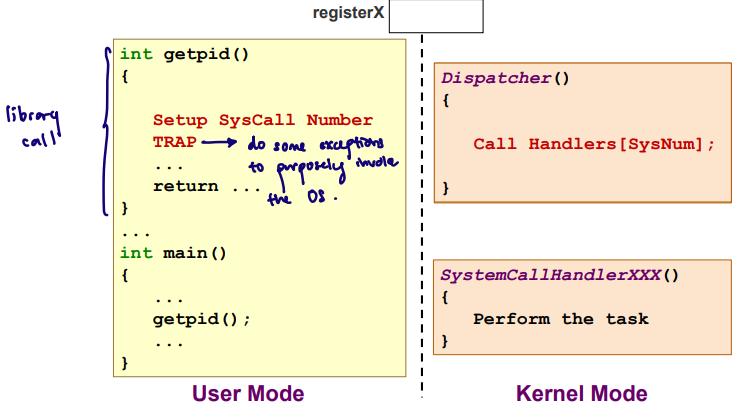
\includegraphics[scale=0.66]{images/syscall.png}

\subsection*{\underline{UNIX Context}}
A UNIX process abstraction has PID for identification, and the following for information:
Process State, Parent PID, Cumulative CPU time (total amount of CPU time used so far) \\
\verb|ps|: short for process status

\verb|init|: Root of all process (UNIX) - PID 1 \\ 

\verb|fork()|: Creates child process with copy of parent's executable image. Child executes remaining code from where the \verb|fork()| was called.
Data not shared. Function returns \verb|0| for child, \verb|> 0| for parent. Child differs in: PID, Parent PID, \verb|fork()| return value. 

% \begin{lstlisting}
%     ... ...
%     int result;                            _
%     result = fork();                        |
%     if (result != 0){                       | 
%         printf("P:My Id is %i\n",           |
%             getpid());                      | Parent
%         printf("P:Child Id is %i\n",        |
%             result);                       _|
%     } else {                               _
%         printf("C:My Id is %i\n",           |
%             getpid() );                     | Child
%         printf("C:Parent Id is %i\n",       | 
%             getppid() );                   _|
%     }
%     ... ...
% \end{lstlisting}

\verb|exec()|: Many variants: \verb|execv, execl, execle, execlv, execlp| Replaces current executing process image with a new one.
Only replaces code, PID and other information remains.
\begin{itemize}[topsep=0pt,noitemsep,wide=0pt, leftmargin=\dimexpr\labelwidth + 2\labelsep\relax, topsep=0pt]
    \item \verb|path|: location of executable, if not executable, return \verb|0|
    \item \verb|arg0, ..., argN|: command line argument(s)
    \item \verb|NULL|: indicate end of argument list
\end{itemize}
% \begin{lstlisting}
%     #include <unistd.h>            // Header file
%                                          _
%     int execl( const char *path,          | 
%                const char *arg0,          | Syntax
%                ...,                       |
%                const char *argN, NULL ); _|
% \end{lstlisting}

\verb|exit()|: Takes in a status, terminates process and returns status to parent process.
Upon process termination, some resourcess are not released: PID, status, CPU time. Generally PCB remains.

% \begin{lstlisting}
%     #include <stdlib.h>       // Header file
%     void exit( int status );  // Syntax
% \end{lstlisting}

\verb|wait()|: Waits for child (blocks), if a child exists, else it returns \verb|-1|. Cleans up on child process 
(those that were nor removed on \verb|exit()|), e.g. removes PCB of child. Also kills \textbf{zombie} processes.
% \begin{lstlisting}
%     #include <sys/types.h>    // Header file  
%     #include <sys/wait.h>     // Header file  
%     int wait( int *status );  // Syntax
% \end{lstlisting}
\begin{itemize}[topsep=0pt,noitemsep,wide=0pt, leftmargin=\dimexpr\labelwidth + 2\labelsep\relax]
    \item \textbf{Zombie:} When child exits but parent doest not call \verb|wait()|
    \begin{itemize}[topsep=0pt,noitemsep,wide=0pt, leftmargin=\dimexpr\labelwidth + 2\labelsep\relax]
        \item On \verb|exit()|, becomes zombie. Cannot delete all process info until \verb|wait()| is called, to allow data to be cleaned up.
    \end{itemize}
    \item \textbf{Orphan:} Subset of Zombie. When parent terminates before child process. \verb|init| becomes parent and does the clean-up
\end{itemize}

\subsection*{\underline{Inter-Process Communication}}
\textbf{P$_1$} creates a shared memory region \textbf{M}. \textbf{P$_2$} attaches memory region \textbf{M} to its own memory space.
\textbf{P$_1$} and \textbf{P$_2$} can now communicate using memory region \textbf{M}. \textbf{M} would behave like a normal memory region.

ADVANTAGES / DISADVANTAGES
\begin{enumerate}[topsep=0pt,noitemsep,wide=0pt, leftmargin=\dimexpr\labelwidth + 2\labelsep\relax, topsep=0pt]
    \item \textbf{Efficient:} Only \verb|create| and \verb|attach| require OS
    \item \textbf{Ease of use:} Shared memory region behaves like a regular one, write info of any size/type
    \item BUT \textbf{Synchronisation} issues and \textbf{Hard to implement}
\end{enumerate}


\subsubsection*{Race Condition}
Final outcome depends on the interleaving of \verb|read| and \verb|write| operations.
Possibly huge number of interleaving scenarios, this could grow exponentially w.r.t number of processes/shared variables/operations on shared variables.

\subsubsection*{Shared Memory (UNIX)}
Basic steps of usage:
\begin{enumerate}[topsep=0pt,noitemsep,wide=0pt, leftmargin=\dimexpr\labelwidth + 2\labelsep\relax, topsep=0pt]
    \item Create/locate a shared memory region \textbf{M}
    \item Attach \textbf{M} to process memory space
    \item Read from/Write to \textbf{M} $\rightarrow$ values written visible to all processes that share \textbf{M}
    \item Detach \textbf{M} from memory space after use
    \item Destory \textbf{M} (only one processes needs to do this) $\rightarrow$ can only destroy if \textbf{M} not attached to any process
\end{enumerate}

\verb|shmget()|: (master) Creates shared memory region, returns the id.

\verb|shmat()|: Attaches shared memory region using the id, and returns a pointer to the region. Done by both master and slave program.

\verb|shmdt()|: Detaches shared memory region using the pointer from attaching. Done by both the master and slave program.

\verb|shmctl()|: Destroys the shared memory region using the id. Generally done by the master program.

\textbf{Master Program} \\ 
\includegraphics*[width=4.2cm, height=3cm]{images/masterprogram.png}
\includegraphics*[width=4.2cm, height=3cm]{images/masterprogram2.png}

\textbf{Worker Program} \\ 
\includegraphics*[width=7cm, height=3cm]{images/workerprogram.png}

\subsubsection*{Message Passing}
\textbf{Naming Scheme}
\begin{enumerate}[topsep=0pt,noitemsep,wide=0pt, leftmargin=\dimexpr\labelwidth + 2\labelsep\relax]
    \item \textbf{Direct Communication:} Sender and receiver explicitly name the other party. Needs one link per pair and processes to know the identity of the other part.
        \begin{itemize}[topsep=0pt,noitemsep,wide=0pt, leftmargin=\dimexpr\labelwidth + 2\labelsep\relax]
            \item \verb|Send(P2, Msg)| - to send \verb|Msg| to process \verb|P2|
            \item \verb|Receive(P1, Msg)| - to receive \verb|Msg| from process \verb|P1|
        \end{itemize}
    \item \textbf{Indirect Communication:} Send and receive from a port. One port can be shared among a number of processes.
        \begin{itemize}[topsep=0pt,noitemsep,wide=0pt, leftmargin=\dimexpr\labelwidth + 2\labelsep\relax]
            \item \verb|Send(MB, Msg)| - to send \verb|Msg| to mailbox \verb|MB|
            \item \verb|Receive(MB, Msg)| - to receive \verb|Msg| from mailbox \verb|MB|
        \end{itemize}
\end{enumerate}

\textbf{Synchronisation} 
\begin{enumerate}[topsep=0pt,noitemsep,wide=0pt, leftmargin=\dimexpr\labelwidth + 2\labelsep\relax]
    \item \textbf{Blocking Primitives (Synchronous):} Also known as \underline{rendezvous}, no intermediate buffering required
        \begin{itemize}[topsep=0pt,noitemsep,wide=0pt, leftmargin=\dimexpr\labelwidth + 2\labelsep\relax]
            \item \verb|send()|: sender is blocked until the message is received
            \item \verb|receive()|: receiver is blocked until a message has arrived
        \end{itemize}
    \item \textbf{Non-Blocking Primitives (Asynchronous):} Too much freedom for programmer, complex program. Finite uffer size means system is not truly async
        \begin{itemize}[topsep=0pt,noitemsep,wide=0pt, leftmargin=\dimexpr\labelwidth + 2\labelsep\relax]
            \item \verb|send()|: sender resumes opertaion immediately
            \item \verb|receive()|: if message hasn't arrived yet, proceeds empty-handed but doesn't block
        \end{itemize}
    \item Usually \verb|receive()| is blocking $\rightarrow$ behavior of sender critical
        \begin{itemize}[topsep=0pt,noitemsep,wide=0pt, leftmargin=\dimexpr\labelwidth + 2\labelsep\relax]
            \item \verb|send()|: blocks until matching \verb|receive()| ran $\rightarrow$ synchronous
            \item \verb|receive()|: proceeds regardless $\rightarrow$ asynchronous
        \end{itemize}
\end{enumerate}

\textbf{Message Buffers} \\ 
Intermediate buffers between sender and receiver in asynchronous communication, under OS control. Large buffer decouples
sender and receiver not need to wait for one another unnecessarily. \\

ADVANTAGES OF MESSAGE PASSING
\begin{enumerate}[topsep=0pt,noitemsep,wide=0pt, leftmargin=\dimexpr\labelwidth + 2\labelsep\relax, topsep=0pt]
    \item \textbf{Portable:} Easily implemented across different processing envs
    \item \textbf{Ease of sync:} Using blocking primitives force sender and receiver to be synchronous
\end{enumerate}

DISADVANTAGES OF MESSAGE PASSING
\begin{enumerate}[topsep=0pt,noitemsep,wide=0pt, leftmargin=\dimexpr\labelwidth + 2\labelsep\relax, topsep=0pt]
    \item \textbf{Inefficient:} Need OS intervention
    \item \textbf{Hard to use:} Messages are limited in size and format
\end{enumerate}
\includegraphics*[width=7.5cm, height=4cm]{images/sharedmemmessagepass.png}

\textbf{Unix Pipes} \\ 
In UNIX, process has 3 default communication channels, \verb|stdin|, \verb|stdout| and \verb|stderr|. The $\vert$
in shell directs one process' output to another's input. e.g. \verb|A| $\vert$  \verb|B|, output of A goes into B.
More generally, a pipe is a FIFO circular bounded byte buffer with implicit synchronisation - writers wait when buffer isolation
full, readers wait when buffer is empty.

\includegraphics*[width=8.5cm, height=4cm]{images/pipe.png}


VARIANTS
\begin{itemize}[topsep=0pt,noitemsep,wide=0pt, leftmargin=\dimexpr\labelwidth + 2\labelsep\relax, topsep=0pt]
    \item Multiple readers and writers
    \item Half-duplex / unidirectional vs full-duplex \ bidirectional
\end{itemize}

\verb|pipe()|: Takes in an integer array of size 2, e.g. \verb|fd[2]|. The resultant \verb|fd[0]| is the reading
end and \verb|fd[1]| is the waiting end.
% \begin{lstlisting}
%     #include <unistd.h>                // Header file  
%     int wait( int pipe( int fd[] ) );  // Syntax
% \end{lstlisting}

\verb|close()|: Takes in a file descriptor and closes it. File descriptor is now unused. \verb|0| is the \verb|stdin|, \verb|1| is the \verb|stdout|, \verb|2| is the \verb|stderr|.

\verb|dup()|: Takes in a file descriptor (fd) and finds the lowest unused fd and duplicates it there. (lowest unused fd is now an alias for the argument fd).
\verb|dup2()|: Like \verb|dup()| execpt that you specify the new file descriptor to duplicate into.

\subsection*{Signal (UNIX)}
An asyncrhonous notification regarding an event sent to a process or a thread. The recipient must either use the default set of handlers
or a user supplied handler to handle the signal.

\verb|signal()|: Takes in a signal and a handler that takes in an argument of type \verb|int| and returns 
\verb|void|, and replaces the default handler with that.

\begin{lstlisting}
void myOwnHandler( int signo ) {    
    if (signo == SIGSEGV) {        
        printf("Memory access blows up!\n");
        exit(1);    
    }
}
int main() {    
    int *ip = NULL;    
    if (signal(SIGSEGV, myOwnHandler) == SIG_ERR) 
        printf("Failed to register handler\n");
    *ip = 123; // seg fault
    return 0;
}
\end{lstlisting}

\subsection*{\underline{Process Scheduling}}
Concept of multiple processes \textbf{progress} in execution (at the same time): virtual / physical parallelism.
1 core (CPU) - Time sliced execution of tasks. OR Multiprocessor: time slicing of \textbf{n} CPUs

\subsection*{Process Behaviour}
\textbf{CPU-Activity:} \\
\begin{itemize}[topsep=0pt,noitemsep,wide=0pt, leftmargin=\dimexpr\labelwidth + 2\labelsep\relax, topsep=0pt]
    \item Computation - e.g. Number crunching
    \item \textbf{Compute-Bound Process} spends majority of its time here
\end{itemize}

\textbf{IO-Activity:} \\ 
\begin{itemize}[topsep=0pt,noitemsep,wide=0pt, leftmargin=\dimexpr\labelwidth + 2\labelsep\relax, topsep=0pt]
    \item Requesting and receiving service from I/O devices - e.g. Print to screen, read from file
    \item \textbf{IO-Bound Processes} spends majority of its time here
\end{itemize}

\subsection*{Processing Environment}
\begin{enumerate}[topsep=0pt,noitemsep,wide=0pt, leftmargin=\dimexpr\labelwidth + 2\labelsep\relax, topsep=0pt]
    \item Batch Processing: No user interaction, no need to be responsive
    \item Interactive / Multiprogramming: With active user interacting system, should be responsive (low/consistent response time)
    \item Real time processing: Have deadline to meet - periodic process 
\end{enumerate}

\subsubsection{Criteria for Scheduling Algorithms}
Largely influenceed by processing environment, may be conflicting \newline
\textbf{Fairness:} Get a fair share of CPU time, per process/user basis \newline
\textbf{Utilization:} All parts of the computing system should be utilized

\subsubsection*{When to perform scheduling}
\textbf{Non-preemptive:} (Cooperative) A process stays scheduled (in running state) untl it blocks or gives up CPU voluntarily
\textbf{Preemptive:} Process given a fixed time quota to run, possible to block / give up early. At the end of time quota, running process suspended, another ready process gets picked.

\framebox{\parbox{\dimexpr\linewidth-2\fboxsep-2\fboxrule}{% 
    $\star$ The moment PC set to one of the addresses of the instruction in a process, it is said to be in the \underline{running} state.

    \begin{enumerate}[topsep=0pt,noitemsep,wide=0pt, leftmargin=\dimexpr\labelwidth + 2\labelsep\relax, topsep=0pt]
        \item Scheduler is triggered (OS takes over)
        \item If context switch needed, context of currently running process is saved and placed on blocked queue / ready queue 
        \item Pick a suitable process \textbf{P} to run based on scheduling algorithm
        \item Setup the context for \textbf{P}, let process \textbf{P} run
    \end{enumerate}
}}

\subsection*{Batch Processing}
No user interaction, non-preemptive scheduling is predominant.

\subsubsection{Criteria for batch processing}
\begin{enumerate}[topsep=0pt,noitemsep,wide=0pt, leftmargin=\dimexpr\labelwidth + 2\labelsep\relax, topsep=0pt]
    \item \textbf{Turnaround time:} Total time taken (finish time - arrival time), related to waiting time (time spent waiting for CPU)
    \item \textbf{Throughput:} Number of tasks finished per unit time (rate of task completion)
    \item \textbf{Makespan:} Total time from start to finish to process all tasks
    \item \textbf{CPU Utilization:} Percentage of time when CPU is working on a task
    \item \textbf{Wait time}: Turnaround time - Burst time
\end{enumerate}

\subsubsection{First-Come First-Served -- Non-Preemptive}
Tasks stored in FIFO queue based on arrirval time. Pick task in queue to run until DONE / BLOCKED. Blocked
task removed from FIFO queue, when ready again place at back of queue.

\framebox{\parbox{\dimexpr\linewidth-2\fboxsep-2\fboxrule}{% 
    $\star$ Guaranteed to have no \textbf{starvation}: number of tasks in front of task X in FIFO is always decreasing.
}}

\textbf{Shortcomings:} Simple reordering can reduce average waiting time - Convoy Effect.

\subsubsection{Shortest Job First (SJF)}
Select task with the smallest total CPU time upon arrival (not preemptive). Need to know total CPU time for a task in advance. Given a fixed set of tasks, minimizes average waiting time.
\framebox{\parbox{\dimexpr\linewidth-2\fboxsep-2\fboxrule}{% 
    $\star$ Starvation is possible as it is biased towards shorter jobs. Long jobs may not get a chance to run.
}}

A task usually goes through several phases of CPU-Activity. Possible to guess the future CPU time requirement by previous CPU-Bound phases.

\begin{itemize}[topsep=0pt,noitemsep,wide=0pt, leftmargin=\dimexpr\labelwidth + 2\labelsep\relax, topsep=0pt]
    \item Actual$_n$ - most recent CPU time consumed
    \item Predicted$_n$ - the previous CPU time consumed
    \item $\alpha$ - Weight placed on recent event or past history
    \item Predicted$_{n+1}$ - Latest prediction
\end{itemize}

\framebox{\parbox{\dimexpr\linewidth-2\fboxsep-2\fboxrule}{% 
    \begin{equation*}
        Predicted_{n+1} = \alpha Actual_n + (1 - \alpha)Predicted_n
    \end{equation*}
}}


\subsubsection{Shortest Remaining Time (SRT) -- Preemptive}
Variation of SJF, use remaining time and preemptive. New job with shorter remaining time can preempt currently running job. Provide good service for short job even when arrived late.

\subsection*{Interactive Systems}
\textbf{Criteria for interactive environment}
\begin{enumerate}[topsep=0pt,noitemsep,wide=0pt, leftmargin=\dimexpr\labelwidth + 2\labelsep\relax, topsep=0pt]
    \item \textbf{Response time:} time between request / response by system
    \item \textbf{Predictability:} variation in response time, lesser variation == more predictable
\end{enumerate}

Preemptive scheduling algorithms are used to ensure good response time $\rightarrow$ scheduler needs to run \textbf{periodically} \newline

\textbf{Interval of Timer Interrupt:}
OS scheduler is invoked on every timer interrupt, typically 1ms to 10ms. (freq of scheduler)

\textbf{Time Quantum:}
Execution duration given to a process, could be constant or variable among the processes. 
Must be multiples of interval of timer interrupt. Large range of values (commonly 5ms to 100ms).
This is the actual time for processes to run.

\subsubsection{Round Robin (RR)}
Tasks stored in a FIFO queue. Pick the first task from queue front to run until fixed \textit{time slice (quantum)} elapsed
or task gives up CPU voluntarily or task blocks. Task is then placed to back of queue to wait another turn. (Block task moved to another queue to wait for requested resource).
When blocked task is ready again, placed at back of queue.

\framebox{\parbox{\dimexpr\linewidth-2\fboxsep-2\fboxrule}{% 
    $\star$ Preemptive version of FCFS.
    \begin{itemize}[topsep=0pt,noitemsep,wide=0pt, leftmargin=\dimexpr\labelwidth + 2\labelsep\relax, topsep=0pt]
        \item Response time guarantee: given \textit{n} tasks and quantum \textit{q}, time before a task gets CPU is bounded by \textit{(n-1)q}
        \item Timer interrupt needed: Scheduler to check on quantum expiry
        \item Choice of time quantum
        \begin{itemize}[topsep=0pt,noitemsep,wide=0pt, leftmargin=\dimexpr\labelwidth + 2\labelsep\relax, topsep=0pt]
            \item Big: Better CPU utilization, longer waiting time
            \item Small: Worse CPU utilization, shorter waiting time
        \end{itemize}
    \end{itemize}
}}

\subsubsection{Priority Scheduling}
Some processes more important than others, assign priority value to all tasks, selecting that with the highest priority value. \\
\textbf{Preemptive:} Higher priority process preempts running process with lower priority \\ 
\textbf{Non-preemptive:} Late coming high priority process has to wait for next round of scheduling

\framebox{\parbox{\dimexpr\linewidth-2\fboxsep-2\fboxrule}{% 
    $\star$ Low prioirty process can starve, high priority process hogging CPU (worse for preemptive version).
    Hard to guarantee or control the exact amount of CPU time given to a process using priority.
}}

Possible solutions:
\begin{itemize}[topsep=0pt,noitemsep,wide=0pt, leftmargin=\dimexpr\labelwidth + 2\labelsep\relax, topsep=0pt]
    \item Decrease priority of currently running process after every quantum (eventually dropped below next highest priority)
    \item Give current running processing a time quantum, not considered in the next round of scheduling
\end{itemize}

\textbf{Priority Inversion:} Lower priority task preempts higher priority \\ 

\begin{itemize}[topsep=0pt,noitemsep,wide=0pt, leftmargin=\dimexpr\labelwidth + 2\labelsep\relax, topsep=0pt]
    \item Priority: \{A=1, B=3, C=5\} (1 highest). Task \textbf{C} starts and locks a resource. \textbf{B} preempts \textbf{C} (unable to unlock resource)\\
    \item Task \textbf{A} arrives and needs same resource as \textbf{C}, but it is locked! 
    \item Task \textbf{B} continues execution even if Task \textbf{A} has higher priority.
\end{itemize}

\subsubsection{Multi-level Feedback Queue (MLFQ)}
\textbf{Adaptive} Learn the process behavior automatically \\
\textbf{Minimizes:} Response time for IO-Bound processes, turnaround time for CPU-Bound processes.

\textbf{Basic Rules:}
\begin{itemize}[topsep=0pt,noitemsep,wide=0pt, leftmargin=\dimexpr\labelwidth + 2\labelsep\relax]
    \item If \verb|Priority(A)| $>$ \verb|Priority(B)| $\rightarrow$ A runs
    \item If \verb|Priority(A)| == \verb|Priority(B)| $\rightarrow$ A and B runs in RR
\end{itemize}

\textbf{Priority Setting/Changing Rules:}
\begin{itemize}[topsep=0pt,noitemsep,wide=0pt, leftmargin=\dimexpr\labelwidth + 2\labelsep\relax]
    \item New job $\rightarrow$ highest priority
    \item If a job fully utilized its time quantum $\rightarrow$ priority reduced
    \item If a job gives up / blocks before finishes its time quantum $\rightarrow$ priority retained
\end{itemize}

\textbf{Abusing MLFQ Algorithm:}
\verb|sleep()| right before the quantum, which is blocking. Since it is no longer using CPU,
the scheduler schedules another task. Ensures that the process always finishes RIGHT BEFORE end of quantum.
This allows process to still retain its high priority.
\begin{itemize}[topsep=0pt,noitemsep,wide=0pt, leftmargin=\dimexpr\labelwidth + 2\labelsep\relax]
    \item \textbf{Solution}: Track total CPU time instead. If we want to further abuse this, we can \verb|fork()| every child process
    to run the task so priority is kept. Parent exits to prevent system from clogging. 
    \item \textbf{Solution to Solution's problem}: Inherit parent's CPU usage statistic, ensure that a child would retain it's parent's priority.
\end{itemize}

\includegraphics*[width=8cm, height=5cm]{images/schedulingtable.jpg}

% 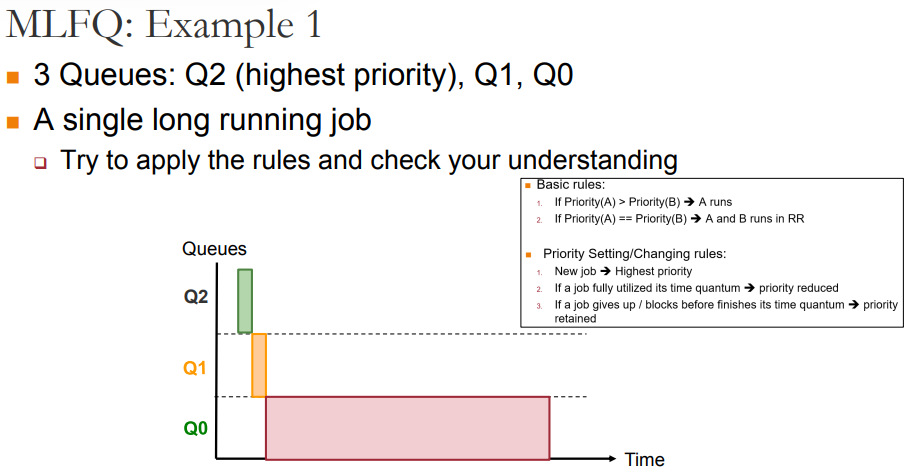
\includegraphics[scale=0.45]{images/mlfq1.png}
% 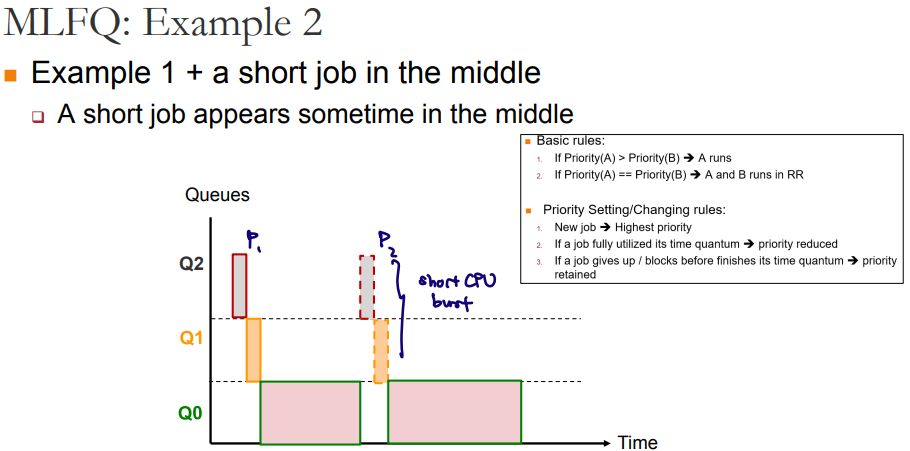
\includegraphics[scale=0.45]{images/mlfq2.png}
% 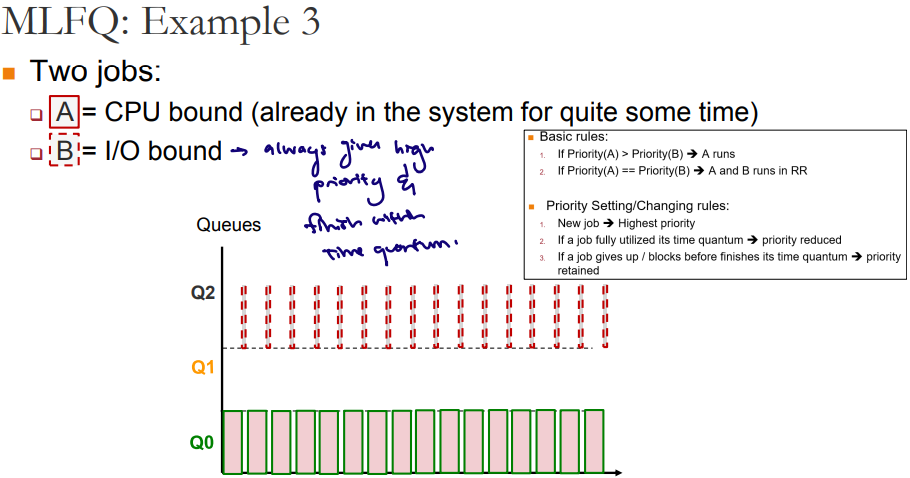
\includegraphics[scale=0.45]{images/mlfq3.png}

\subsubsection{Lottery Scheduling}    

Give out `lottery tickets' to processes for various system resources. When a scheudling decision is needed,
lottery ticket is chosen \underline{randomly among eligible tickets}, winner granted resource. In 
the long run, a process holding \textbf{X}\% of tickets can win \textbf{X}\% of lottery held, and it uses the resources \textbf{X}\% of the time

\begin{itemize}[topsep=0pt,noitemsep,wide=0pt, leftmargin=\dimexpr\labelwidth + 2\labelsep\relax]
    \item \textbf{Responsive:} newly created process can participate in the next lottery
    \item \textbf{Good level of control:} Process can be given Y lottery tickets, distribute to child process
    \item \textbf{Important process given more lottery tickets}
    \item \textbf{Each resouce can have its own set of tickets}
    \item \textbf{Simple to implement}
\end{itemize}

\subsection*{\underline{Synchronisation Primitives}}
Execution of single sequential process is \textit{deterministic}. However execution of 
concurrent processes may be \textbf{non-deterministic} as the execution outcome depends on the
order in which the shared resources is accessed or modifed.


\subsection*{Race Condition Solution}
\textbf{Needed}: synchronization to control the interleaving of accesses to a shared resource.
\begin{itemize}[topsep=0pt,noitemsep,wide=0pt, leftmargin=\dimexpr\labelwidth + 2\labelsep\relax]
    \item Allow all (as many as possible) correct interleaving scenarios
    \item Not allow any incorrect interleaving scenario
\end{itemize}

\subsubsection{Solution Outline}
\begin{itemize}[topsep=0pt,noitemsep,wide=0pt, leftmargin=\dimexpr\labelwidth + 2\labelsep\relax]
    \item Desginate code segment with race condition as \underline{critical section}
    \item At most 1 process in critical section
\end{itemize}

\subsection*{Critical Section}
\subsubsection*{Properties of CS}
\begin{itemize}[topsep=0pt,noitemsep,wide=0pt, leftmargin=\dimexpr\labelwidth + 2\labelsep\relax]
    \item \textbf{Mutual Exclusion}: If process \verb|P| is executing in critical section, all other processes are prevented from entering critical section.
    \item \textbf{Progress}: If no process in critical section, one of the waiting processes should be granted accesses.
    \item \textbf{Bounded Wait}: After process \verb|P| request to enter critical section, there exist an upper bound on the number of times other processes can enter the critical section before \verb|P|.
    \item \textbf{Independence}: Process not executing in critical section should never block other processes.
\end{itemize}

\subsubsection*{Symptoms of Incorrect Synchronisation}
\begin{itemize}[topsep=0pt,noitemsep,wide=0pt, leftmargin=\dimexpr\labelwidth + 2\labelsep\relax]
    \item \textbf{Incorrect output/behaviour} - to lack of Mutual Exclusion
    \item \textbf{Deadlock} - all processes blocked (circular dependency loop) $\rightarrow$ no progress
    \item \textbf{Livelock} - Process not in a blocked state, keep changing state to avoid deadlock but make no progress.
    Usually related to \textit{deadlock avoidance}.
    \item \textbf{Starvation} - processes blocked forever, algo is favouring certain processes
\end{itemize}

\textbf{Peterson's Algorithm}:
\begin{multicols*}{2}
\begin{lstlisting}
// Process 1
Want[0] = 1;
Turn = 1;
while (Want[1] 
    && Turn == 1);
// CRITICAL SECTION
Want[0] = 0
\end{lstlisting}
\begin{lstlisting}
// Process 1
Want[1] = 1;
Turn = 0;
while (Want[0] 
    && Turn == 0);
// CRITICAL SECTION
Want[1] = 0
\end{lstlisting}
\end{multicols*}

\begin{itemize}[topsep=0pt,noitemsep,wide=0pt, leftmargin=\dimexpr\labelwidth + 2\labelsep\relax]
    \item If ONLY the \verb|Turn| based system. P0 and P1 takes turn to enter the \textbf{critical section}.
    This could lead to starvation as if P0 never enters CS, P1 starves, violating the \underline{independence} property.
    \item If ONLY the \verb|Want[]| based system. P0 or P1 not around, another process can still enter CS, however could result in a DEADLOCK, violating the \underline{progress} property.    
    Both systems wanting, repeated the while loop.
\end{itemize}

\subsection*{Assembly Level Implementation}
\textbf{Test and Set:} Atomic/machine instruction, aid synchronisation.
\textbf{Behavior:} Entirely behaves like a single atomic machine operation (cannot be broken).
\begin{itemize}[topsep=0pt,noitemsep,wide=0pt, leftmargin=\dimexpr\labelwidth + 2\labelsep\relax]
    \item Load the current content at \verb|MemoryLocation| into \verb|Register|
    \item Store a \underline{1} into \verb|MemoryLocation|
\end{itemize}
\begin{lstlisting}
void EnterCS(int* Lock) { 
    while (TestAndSet( Lock ) == 1); 
}
void ExitCS(int* Lock) { *Lock = 0; }

/* Process P0 */         | /* Process P1 */
EnterCS();x+=1;ExitCS(); | EnterCS();x+=1;ExitCS();
\end{lstlisting}

Employs busy waiting, keeps checking the condition until it is safe to enter, might waste processing power.
Does not guarantee bounded-wait out of the box (unless scheduling) is fair.

\subsubsection*{Semaphore}
\textbf{S} contains int value, can be initialized to any non-negative values.
\begin{itemize}[topsep=0pt,noitemsep,wide=0pt, leftmargin=\dimexpr\labelwidth + 2\labelsep\relax]
    \item \verb|Wait( S )|: If \verb|S| $\leq$ 0, blocks (go to sleep), Decrement \verb|S|. -- aka \verb|P()| or \verb|Down()|
    \item \verb|Signal( S )|: Increments \verb|S|, wakes up one sleeping process if any, this operation \textbf{never blocks}. -- aka \verb|V()| or \verb|Up()|
\end{itemize}

Given \verb|S >= 0|, then the following \textbf{invariant} must be true:
\framebox{\parbox{\dimexpr\linewidth-2\fboxsep-2\fboxrule}{% 
\begin{equation*}
    S_{current} = S_{initial} + \#signal(S) - \#wait(S)
\end{equation*}
}}
\verb|#signal(S)| -- number of signal() operations executed \newline
\verb|#wait(S)| -- number of wait() operations completed

\cprotect\textbf{Binary Semaphores \verb|S = 1|}
\textbf{S  an only be 0} or \textbf{1}. (aka MUTEX, mutual exclusion)

\subsubsection{Priority Inversion Solution}
Priority inheritance
\begin{itemize}[topsep=0pt,noitemsep,wide=0pt, leftmargin=\dimexpr\labelwidth + 2\labelsep\relax]
    \item Temporarily increase priority of L - H $\rightarrow$ Until unlocks the lock
    \item Low-priority job inherits priority of higher priority process
    \begin{multicols*}{2}
    
    \begin{itemize}[topsep=0pt,noitemsep,wide=0pt, leftmargin=\dimexpr\labelwidth + 2\labelsep\relax]
        \item Happens when the high-priority process requests a lock        held by low-priority process
        \item Priority restored upon successful unlock()
    \end{itemize}

        EXAMPLE: The highest and lowest priority tasks running code A and a middle priority task
        running task B. \vfill\null \columnbreak 

        \begin{lstlisting}
// Code A
wait(S);
<do some work>
signal(S);

// Code B
<heavy computation>
        \end{lstlisting}
    \end{multicols*}
\end{itemize}


\subsection*{\underline{Process Alternative - Threads}}
Processes are expensive as when creating child processes using \verb|fork()|, it 
duplicates both \underline{memory space} and \underline{process context}. Context
switch also requires saving/restoration of process information.

Independent processes have no easy way to pass information to one another,
and requires IPC. These requires syscalls to be done which are also expensive.

\subsection*{Multiple threads of control}
\textbf{Using fork() vs threads}
\begin{lstlisting}
int result;             | int main() {
result = fork();        |   Thread 1 { steamRice() };
if (result != 0) {      |   Thread 2 { fryFish() };
    result = fork();    |   Thread 3 { cookSoup() };
    if (result != 0) {  |   Wait all threads finish;
        steamRice();    |   printf("Lunch Ready\n");
    } else {            |   return 0
        fryFish();      | }
    }                   |
} else {                |
    cookSoup();         |
}                       |
\end{lstlisting} 

\subsection*{Process and Thread}
\begin{itemize}[topsep=0pt,noitemsep,wide=0pt, leftmargin=\dimexpr\labelwidth + 2\labelsep\relax]
    \item A single process can have multiple threads, threads of same process shares:
    \begin{itemize}[topsep=0pt,noitemsep,wide=0pt, leftmargin=\dimexpr\labelwidth + 2\labelsep\relax]
        \item \textbf{Memory Context:} Text, Data Heap
        \item \textbf{OS Context:} Process id, other resources like files, etc.
    \end{itemize}
    \item Unique Information needed for each thread:
    \begin{itemize}[topsep=0pt,noitemsep,wide=0pt, leftmargin=\dimexpr\labelwidth + 2\labelsep\relax]
        \item Identification (usually \textbf{thread id}), Registers (General purpose and special)
        \item "Stack" -- Stack and CPU cannot be shared. Each thread implemented like a function
        thus each thread should hvae its own stack and store its own local data and values.
    \end{itemize} 
\end{itemize}

\subsubsection*{Process Context Switch vs Thread Switch}
\begin{itemize}[topsep=0pt,noitemsep,wide=0pt, leftmargin=\dimexpr\labelwidth + 2\labelsep\relax]
    \item Process Context switch involves:
    \begin{itemize}[topsep=0pt,noitemsep,wide=0pt, leftmargin=\dimexpr\labelwidth + 2\labelsep\relax]
        \item OS Context: syscalls
        \item Hardware Context: Register values change
        \item Memory Context: Remove process from memory and place in a different place
    \end{itemize}
    \item Thread switch within the same process involves:
    \begin{itemize}[topsep=0pt,noitemsep,wide=0pt, leftmargin=\dimexpr\labelwidth + 2\labelsep\relax]
        \item Hardware context: Registers and "Stack" -- changing FP and SP registers
    \end{itemize}
\end{itemize}

\subsubsection{Benefits of Threads}
\begin{enumerate}[topsep=0pt,noitemsep,wide=0pt, leftmargin=\dimexpr\labelwidth + 2\labelsep\relax]
    \item Economy: Multiple threads require much less resource than multiple processes
    \item Resource sharing: Share most of the resources in a process, no need for IPC to pass information 
    \item Responsiveness: Multi-threaded programs can appear more responsive
    \item Scalability: Multi-threaded programs can take advantage of multiple CPUs
\end{enumerate}

\subsubsection{Problems of Threads}
\begin{enumerate}[topsep=0pt,noitemsep,wide=0pt, leftmargin=\dimexpr\labelwidth + 2\labelsep\relax]
    \item \textbf{System Call Concurrency}: Parallel execution of multiple threads $\rightarrow$ parallel syscall possible.
    Have to gurantee correctness and determine the correct behaviour.
    \item \textbf{Process Behavior}: Impact on process operations. \verb|fork()|, \verb|exit()| and \verb|exec()| called on a single thread,
    what about other threads or other processes.
\end{enumerate}

\subsection*{User Thread}
Thread is implemented as a \textbf{user library}. A runtime system (in the process) handles thread related operation.
Kernel is \textbf{NOT AWARE} of the threads in a process. \\

ADVANTAGES
\begin{itemize}[topsep=0pt,noitemsep,wide=0pt, leftmargin=\dimexpr\labelwidth + 2\labelsep\relax]
    \item Can have multi-threaded program on ANY OS
    \item Thread operation are just library calls
    \item Generally more configurable and flexible
\end{itemize}

DISADVANTAGES
\begin{itemize}[topsep=0pt,noitemsep,wide=0pt, leftmargin=\dimexpr\labelwidth + 2\labelsep\relax]
    \item OS unaware of threads, scheduling performed at process level
    \item One thread blocked $\rightarrow$ Process blocked $\rightarrow$ all threads blocked, cannot exploit multiple CPU
\end{itemize}

\subsection*{Kernel Thread}
Thread is implemented in the OS, thread operations handled as system calls. Thread-level scheduling
is possible (schedules by threads instead of processes.) Kernel may make use of threads
for own execution. \\

ADVANTAGES
\begin{itemize}[topsep=0pt,noitemsep,wide=0pt, leftmargin=\dimexpr\labelwidth + 2\labelsep\relax]
    \item Kernel can schedule on thread levels: More than 1 thread in the same process can run simultaneously on multiple CPUs
\end{itemize}

DISADVANTAGES
\begin{itemize}[topsep=0pt,noitemsep,wide=0pt, leftmargin=\dimexpr\labelwidth + 2\labelsep\relax]
    \item Thread operations are now a syscall: slower, more resource intensive. Less flexible: Used by all multi-threaded processes
\end{itemize}

% \includegraphics*[width=8.5cm, height=4cm]{images/userthread.png}
% \includegraphics*[width=8.5cm, height=4cm]{images/kernelthread.png}

\subsubsection{Hybrid Thread Model}
Have both Kernel and User threads. OS can schedule on kernel threads only. We can have
the User thread bind to a Kernel Thread. Offers greater flexibility, limiting concurrency of any process or user.

\begin{itemize}[topsep=0pt,noitemsep,wide=0pt, leftmargin=\dimexpr\labelwidth + 2\labelsep\relax]
    \item 1-1 binding in hybrid thread model, acts more like a pure kernel thread, since kernel threads can be scheduled.
\end{itemize}

\textbf{Hardware Support on Modern Processes:} Supply multiple sets of registers (GPRs, Special registers) to allow threads
to run natively and in parallel on the same core $\rightarrow$ simultaneous multi-threading (SMT) or hyperthreading on Intel processor.

\subsection*{POSIX Threads}
% \begin{lstlisting}
% #include <pthread.h>           // Header file
                                        
% gcc XXXX.c -lpthread           // Compilation
% pthread_t    // Represent a thread id (TID)
% pthread_attr // Represent attributes of a thread
% \end{lstlisting}

\begin{lstlisting}
int pthread_create( // 0 = success, !0 = error
    pthread_t* tidCreated, // threadId 
    const pthread_attr_t threadAttribtues, // control behaviour
    void* (*startRoutine) (void*). //pointer to fn
    void* argForStartRoutine ); 
\end{lstlisting}

\begin{lstlisting}
int pthread_exit( void* exitValue );
\end{lstlisting}
    \begin{itemize}[topsep=0pt,noitemsep,wide=0pt, leftmargin=\dimexpr\labelwidth + 2\labelsep\relax]
        \item If \verb|pthread_exit()| is not used, pthread terminate automatically at end of \verb|startRoutine|. 
        If a "return XYZ;" statement is not used, then "XYZ" captured as exitValue
        \item Otherwise, exitValue not well defined
    \end{itemize}


\subsubsection{pthread Synchronisation}
\begin{lstlisting}
int pthread_join( pthread_t threadId, 
    void **status ); // exit value returned by threadId
    // used to wait for termination of another pthread
\end{lstlisting}

\subsection{\underline{Classical Synchronisation Problems}}

\subsubsection{Producer-Consumer}
Process share a bounded buffer of size \textbf{K}. Producers only produce items to insert in buffer
when the buffer is not full. Consumers removes items from buffer, only when buffer is not empty.

\begin{lstlisting}
//zeroUponFull = N, zeroUponEmpty = 0
//Produce            | //Consume
wait(zeroUponFull)   | wait(zeroUponFull)
wait(mutex)          | wait(mutex)
buffer[in] = item    | buffer[out] = item 
in = (in + 1) % N    | out = (out + 1) % N 
signal(mutex)        | signal(mutex)
signal(zeroUponEmpty)| signal(zeroUponEmpty)
\end{lstlisting} 


\subsubsection{Readers Writers}
The solution allows either one writer or multiple readers in the “room”. It works but can cause starvation of the writer.

\begin{lstlisting}
wait(roomLock)      | wait(mutex)  
//Write data        | nReader++ 
signal(roomLock)    | if nReader == 1: 
                    |   wait(roomLock)
                    | signal(mutex)
                    | //Read data
                    | wait(mutex)
                    | nReader--
                    | if nReader == 0: 
                    |   signal(roomLock)
                    | signal(mutex)
\end{lstlisting} 

\subsubsection{Dining Philosophers}
5 philosophers seated around a table, 5 single chopsticks placed between each pair of philosophers. 
When any philosophers wants to eat, they will have to acquire both chopsticks to their right.
\begin{itemize}[topsep=0pt,noitemsep,wide=0pt, leftmargin=\dimexpr\labelwidth + 2\labelsep\relax]
    \item \textbf{deadlock-free}, \textbf{starve-free} to allow philosophers to eat freely.
\end{itemize}

% ATTEMPT 1 \\
% \begin{multicols*}{2}
%     \includegraphics*[width=4.3cm, height=5cm]{images/diningphilosophers.png}
%     \begin{itemize}[topsep=0pt,noitemsep,wide=0pt, leftmargin=\dimexpr\labelwidth + 2\labelsep\relax]
%         \item \textbf{Deadlock problem:} All philosophers simultaneously take left chopstick, no one can proceed.
%         \item \textbf{Fix attempt:} Make each philosopher put down left chopstick if right chopstick is used.
%         \item Results in a \textbf{livelock:} Pickup left chopstick, put down if its taken, pick up again and repeat...
%     \end{itemize}
% \end{multicols*}

% ATTEMPT 2 \\
% \begin{multicols*}{2}
%     \includegraphics*[width=4cm, height=3.8cm]{images/diningphilosophers2.png}
%     \begin{itemize}[topsep=0pt,noitemsep,wide=0pt, leftmargin=\dimexpr\labelwidth + 2\labelsep\relax]
%         \item This works but it kills concurrency, as only 1 philosophers can dine at once.
%         \item We can solve this if we limit the number of philisophers (to 4) or have one of the philosopher pick up the chopstick on the right first instead.
%     \end{itemize}
% \end{multicols*}
% \begin{itemize}[topsep=0pt,noitemsep,wide=0pt, leftmargin=\dimexpr\labelwidth + 2\labelsep\relax]
%     \item R can grab both right and left chopstick, R eats $\rightarrow$ no deadlock
%     \item R grabbed right chopstick, left chopstick taken, THEN left neighbour has both chopsticks $\rightarrow$ eating $\rightarrow$ eventually will release chopsticks
%     \item R cannot grab right chopstick, right neighbour has left chopstick. Worst case scenario: all 
%     remaining left-handers hold on to their left chopsticks. However, the left neighbor of R 
%     will be able to take its right chopstick because R is still trying to get its right chopstick. 
% \end{itemize}

TANENBAUM SOLUTION 
\begin{multicols*}{2}
    \includegraphics*[width=4cm, height=4.5cm]{images/tanenbaum1.png}
    \includegraphics*[width=4.5cm, height=4.5cm]{images/tanenbaum2.png}
\end{multicols*}
\begin{multicols*}{2}
    \includegraphics*[width=4cm, height=4.5cm]{images/tanenbaum3.png} 
    \begin{itemize}[topsep=0pt,noitemsep,wide=0pt, leftmargin=\dimexpr\labelwidth + 2\labelsep\relax, topsep=0pt]
        \item Previously we block on the chopstick $\rightarrow$ which is between 2 philosophers.
        \item This solution, each philosopher has its own semaphore, which blocks itself if its partners are eating.
        \item Being blocked waiting on others could cause a deadlock, this solution gurantees no deadlock.
        \item OR: 4 seated philisophers, treating pickup of both chopsticks as atomic, or asymmetric (one pick left, one pick right first)
    \end{itemize}
\end{multicols*}

\subsection{\underline{Memory Abstraction}}

% \subsubsection*{Fix Attempt: Address Relocation}
% \begin{multicols*}{2}
%         Recalculate the memory references during program loading. However, this will cause process \underline{start-up} time to increase (slow loading)!

%         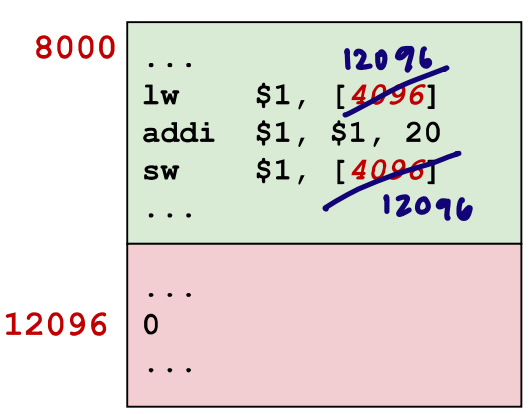
\includegraphics[width=3cm, height=1cm]{images/addressrelocation.png}
% \end{multicols*}

% \subsubsection*{Fix Attempt 2: Base + Limit Registers}
% \begin{enumerate}[topsep=0pt,noitemsep,wide=0pt, leftmargin=\dimexpr\labelwidth + 2\labelsep\relax]
%     \item Use special register as the base of all memory references 
%     \begin{itemize}[topsep=0pt,noitemsep,wide=0pt, leftmargin=\dimexpr\labelwidth + 2\labelsep\relax]
%         \item During compile time, all memory references compiled as an offset from this register
%         \item At loading time, the base register is initialized to the starting address of the process memory space
%     \end{itemize}
%     \item Add another special register to indicate the range of the memory space of current process
%     \begin{itemize}[topsep=0pt,noitemsep,wide=0pt, leftmargin=\dimexpr\labelwidth + 2\labelsep\relax]
%         \item Limit Register, every memory access is checked against the limit to protect memory space intergrity
%     \end{itemize}
% \end{enumerate}

% PROBLEMS
% \begin{itemize}[topsep=0pt,noitemsep,wide=0pt, leftmargin=\dimexpr\labelwidth + 2\labelsep\relax]
%     \item To access \verb|Addr|, \verb|Actual| = \verb|Base| + \verb|Addr|
%     \item Check \verb|Actual| $<$ \verb|Limit|
%     \item Every memory access incurs an addition and comparison
% \end{itemize}

\subsection*{Contiguous Memory Management}
Process must be in memory as one piece during the whole execution. To support \textit{multitasking}
we allow multiple processes in the physical memory at the same time (switch from one to another). When physical
memory is full, we free up memory by removing terminated processes, or swapped blocked processes to secondary storage.

\subsection*{Memory Partitioning}
\textbf{Fixed Partitioning:} Leftover space is wasted for any process that does not occupy whole partition: \textit{\textbf{internal fragmentation}}\\
\begin{itemize}[topsep=0pt,noitemsep,wide=0pt, leftmargin=\dimexpr\labelwidth + 2\labelsep\relax]
    \item \textbf{Pros:} Easy to manage, fast to allocate. Every free partition is the same (no choosing needed).
    \item \textbf{Cons:} Partition size needs to be large enough to contain the largest of processes $\rightarrow$ smaller process will waste memory space.
\end{itemize}

\textbf{Dynamic Partitioning:}Free memory space is known as \textbf{hole}. With process creation, termination or swapping tend to have large number of holes, also known as: \textit{\textbf{external fragmentation}}\\
\begin{itemize}[topsep=0pt,noitemsep,wide=0pt, leftmargin=\dimexpr\labelwidth + 2\labelsep\relax]
    \item \textbf{Pros:} Flexible and remove internal fragmentation.
    \item \textbf{Cons:} Need to maintain information in OS, takes more time to locate appropriate region.
\end{itemize}

\subsection*{Allocation Alrogithms}
Assume OS maintain list of partitions and holes, algorithm to locate partition of size \verb|N|. Search for hole with size \verb|M| $>$ \verb|N|.
\begin{itemize}[topsep=0pt,noitemsep,wide=0pt, leftmargin=\dimexpr\labelwidth + 2\labelsep\relax]
    \item \textbf{\textit{First-Fit}:} Take first hole large enough, minimize search time.
    \item \textbf{\textit{Best-Fit}:} Take smallest hole large, reduce size of hole created.
    \item \textbf{\textit{Worst-Fit}:} Find largest hole, make bigger hole for future process after partition.
    \item \verb|N| will be new partition, \verb|M - N| will be left over space
\end{itemize}

\subsubsection*{Reducing External Fragmentation}
\begin{itemize}[topsep=0pt,noitemsep,wide=0pt, leftmargin=\dimexpr\labelwidth + 2\labelsep\relax]
    \item \textbf{Merge:} Occupied partition freed, merge with adjacent hole.
    \item \textbf{Compaction:} Move occupied partitions around to create bigger consolidated holes $\rightarrow$ cannot be invoked too frequently as it is very time consuming.
\end{itemize}


\subsection*{Multiple Free Lists}
\begin{multicols*}{2}
    \begin{itemize}[topsep=0pt,noitemsep,wide=0pt, leftmargin=\dimexpr\labelwidth + 2\labelsep\relax]
        \item Separate list of free holes from list of occupied partitions
        \item Keep multiple lists of different hole sizes
    \end{itemize}

    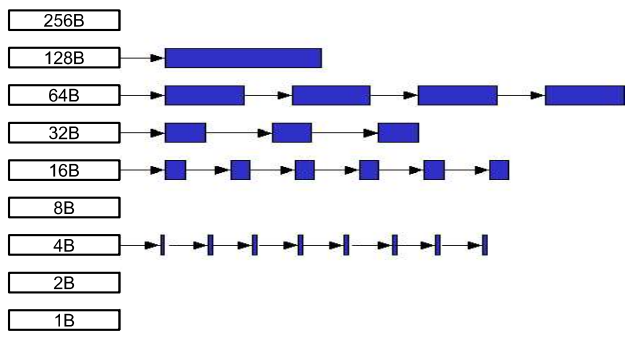
\includegraphics[width=4.2cm, height=1.3cm]{images/multifreelists.png}
\end{multicols*}

\subsubsection*{Buddy System}
\begin{itemize}[topsep=0pt,noitemsep,wide=0pt, leftmargin=\dimexpr\labelwidth + 2\labelsep\relax]
    \item \textbf{Buddy} memory allocation provides efficient partition splitting, locating good match for free partition (hole), partition de-allocation and coalescing
    \item \textbf{Main Idea:}
    \begin{itemize}[topsep=0pt,noitemsep,wide=0pt, leftmargin=\dimexpr\labelwidth + 2\labelsep\relax]
        \item Free block is split into half repeatedly to meet request size
        \item 2 halves forms a sibling blocks (buddy blocks)
        \item When buddy blocks \textbf{both free}, merged into larger block
    \end{itemize}
\end{itemize}

% \textbf{Buddy System Allocation Algorithm} \\ 
% \begin{enumerate}[topsep=0pt,noitemsep,wide=0pt, leftmargin=\dimexpr\labelwidth + 2\labelsep\relax]
%     \item Find smallest \verb|S| such that \verb|2^s >= N|
%     \item Access \verb|A[S]| for free block
%     \item If free block exists: remove block from free block list and allocate the block
%     \item Else: Find smallest \verb|R| from \verb|S+1| to \verb|K| s.t. \verb|A[R]| has free block \verb|B|. Repeatedly split B such that there is a new block and go to step 2
% \end{enumerate}

% 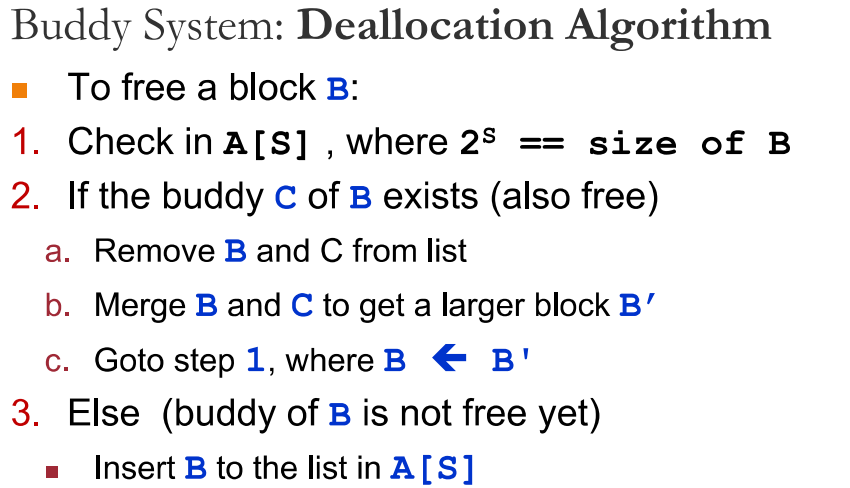
\includegraphics[width=8.5cm, height=3.4cm]{images/buddydeallocation.png}
% 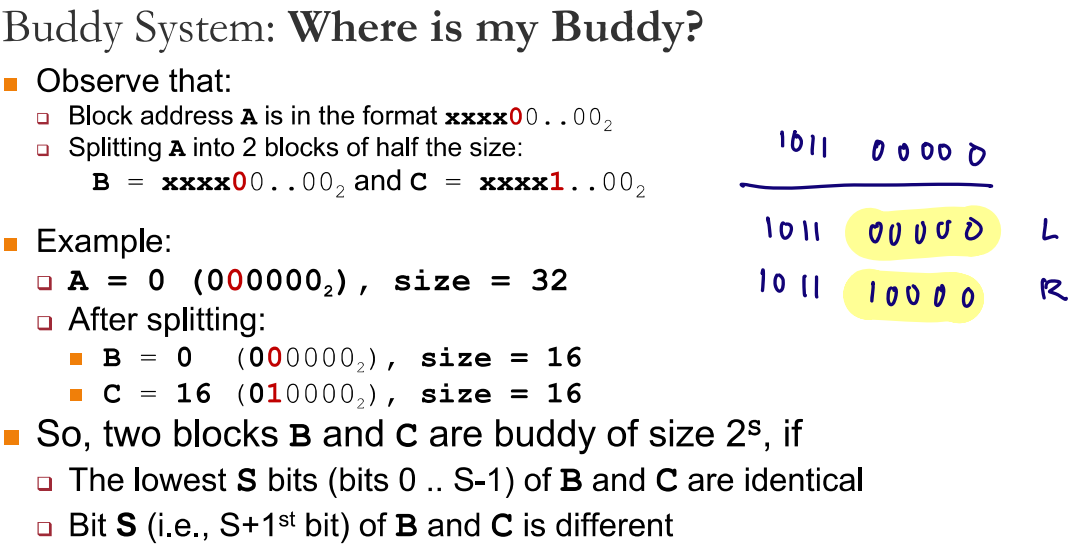
\includegraphics[width=8.5cm, height=4cm]{images/buddyfind.png}

\subsection{\underline{Disjoint Memory Schemes}}
\begin{itemize}[topsep=0pt,noitemsep,wide=0pt, leftmargin=\dimexpr\labelwidth + 2\labelsep\relax]
    \item Logical page $\leftrightarrow$ physical page (frame) mapping not as straightforward
    \item Need a lookup table to provide translation: \textbf{page table}
\end{itemize}

\begin{itemize}[topsep=0pt,noitemsep,wide=0pt, leftmargin=\dimexpr\labelwidth + 2\labelsep\relax]
    \item Physical Add = \textit{FrameNum} $\times$ \verb|sizeof|(physicalframe) + \textit{offset}
    \item Offset is the displacement from beginning of the physical frame
    \item Frame sizes (page size) as a power-of-2 $\rightarrow$ for bit level addressing
\end{itemize}


\subsubsection*{Formula}
\begin{itemize}[topsep=0pt,noitemsep,wide=0pt, leftmargin=\dimexpr\labelwidth + 2\labelsep\relax]
    \item Given: Page/Frame size of \verb|2^n|, \verb|n| bits of logical addresses
    \item Logical Address \verb|LA|:
    \begin{itemize}[topsep=0pt,noitemsep,wide=0pt, leftmargin=\dimexpr\labelwidth + 2\labelsep\relax]
        \item \verb|p| = Most significant \verb|m-n| bits of \verb|LA|
        \item \verb|o| = Remaining \verb|n| bits of \verb|LA|
    \end{itemize}
    \item Use \verb|p| to find frame number \verb|f| from mapping mechanism like page table
    \item Physical Address \verb|PA|: \verb|PA = f * 2^n + o|
\end{itemize}

\begin{itemize}[topsep=0pt,noitemsep,wide=0pt, leftmargin=\dimexpr\labelwidth + 2\labelsep\relax]
    \item \textbf{External Fragmentation:} Not possible, no left-over physical memory region, every single free frame can be used
    \item \textbf{Internal Fragmentation:} Logical memory space not multiple of page size, max one page per process not fully utilized
    \item Clean separation of \textit{logical} and \textit{physical} address space, good flexibility and simple address translation
\end{itemize}

\subsubsection*{Paging Scheme Implementation}
\begin{itemize}[topsep=0pt,noitemsep,wide=0pt, leftmargin=\dimexpr\labelwidth + 2\labelsep\relax]
    \item \textbf{Pure-software} solution, OS stores page table information in PCB, memory context of process includes the page table
    \item Issues: requires 2 memory access for every memory reference (1 to red indexed page table entry to get frame number, 2 to access actual memory item) || HUGE OVERHEAD
\end{itemize}

\subsection*{Translation Look-Aside Buffer (TLB)}
\begin{itemize}[topsep=0pt,noitemsep,wide=0pt, leftmargin=\dimexpr\labelwidth + 2\labelsep\relax]
    \item \textbf{TLB} provided by modern processors, specialized on-chip component to stop paging.
    \item TLB acts as \textbf{cache} for page table entries, reducing redudnat access, very small (10s of entries) and fast ($<$= 1 clock cycle)
\end{itemize}

\underline{Logical-to-physical address translation with TLB}
\begin{itemize}[topsep=0pt,noitemsep,wide=0pt, leftmargin=\dimexpr\labelwidth + 2\labelsep\relax]
    \item Use page number to search TLB associatively
    \begin{itemize}[topsep=0pt,noitemsep,wide=0pt, leftmargin=\dimexpr\labelwidth + 2\labelsep\relax]
        \item \textbf{TLB-Hit}: Frame number to generate physical address
        \item \textbf{TLB-Miss}: Memory access to access the page table, retrieved frame number used to generated physical address and update TLB
    \end{itemize}
\end{itemize}

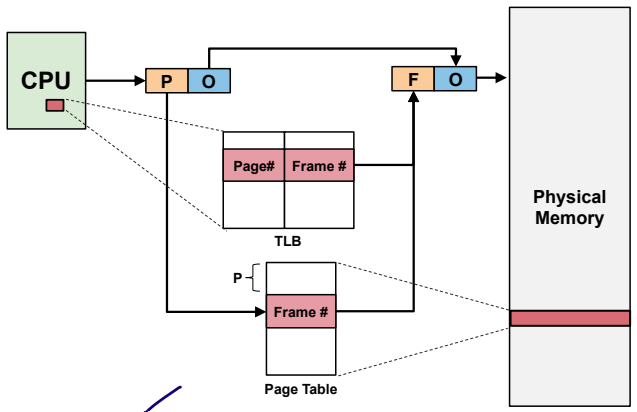
\includegraphics[width=8.5cm, height=4cm]{images/tlb.png}
\subsubsection*{TLB: Impact on Memory Access Time}
TLB access takes \textbf{1ns}, main memory access takes \textbf{50ns}, average memory access time if hit ratio is 90\%:
\begin{equation*}
    \begin{array}{l}
        P(TLB hit) \times latency(TLB hit) + P(TLB miss) \times latency(TLB miss) \\ 
        = 90\% \times (1 + 50) + 10\% \times (1 + 50 + 50) = 56 ns 
    \end{array}
\end{equation*}

\subsubsection*{TLB and Process Switching}
1 TLB for every physical core (minimally), on context switch:
\begin{itemize}[topsep=0pt,noitemsep,wide=0pt, leftmargin=\dimexpr\labelwidth + 2\labelsep\relax]
    \item TLB entries flushed, new process won't get incorrect translation
    \item Avoids correctness, security and safety issues
    \item When a process resumes running, encounter many TLB misses to fill TLB
\end{itemize} 

\subsection*{Paging Scheme: Protection}
\begin{itemize}[topsep=0pt,noitemsep,wide=0pt, leftmargin=\dimexpr\labelwidth + 2\labelsep\relax]
    \item \textbf{\textit{Access-Right Bits}}
    \begin{itemize}[topsep=0pt,noitemsep,wide=0pt, leftmargin=\dimexpr\labelwidth + 2\labelsep\relax]
        \item Page Table Entry has \underline{writable, readable, executable} bits
        \item Page containing code: \textbf{executable and read only}
        \item Page containing data: \textbf{readable and writable}
        \item Every memory access checked against access bits in hardware
    \end{itemize}
    \item \textbf{\textit{Valid Bit}}: Logical memory range is the same for all processes, not all processes utilize the whole range, some pages out-of-range for a particular process
    \begin{itemize}[topsep=0pt,noitemsep,wide=0pt, leftmargin=\dimexpr\labelwidth + 2\labelsep\relax]
        \item Indicate whether the page is valid to access by the process
        \item OS set valid bits as memory is being allocated to the process
        \item \textit{Every} memory access checked against this bit in hardware, out-out-range access caught by OS
    \end{itemize}
\end{itemize}

\subsubsection*{Page Sharing}
\begin{itemize}[topsep=0pt,noitemsep,wide=0pt, leftmargin=\dimexpr\labelwidth + 2\labelsep\relax]
    \item Shared code page, some code is being used by many processes: C standard lib, syscalls etc.
    \item Implementing \textbf{Copy-On-Write}: parent and child process can share a page until 1 tries to change a value in it. Mark all pages a READ-ONLY when copied, generate exception if Q wants to write. OS catches, can generate a new copy of pages for Q to write on.
\end{itemize}

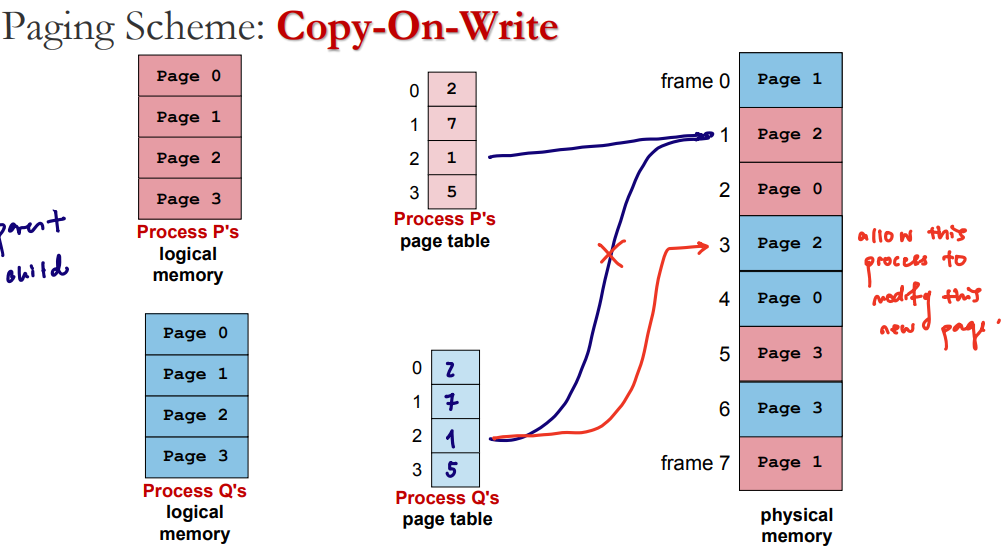
\includegraphics[width=8.5cm, height=4cm]{images/copyonwritepaging.png}

\subsection*{Segmentation Scheme}
Manage memory at level of \textbf{memory segments}
\begin{itemize}[topsep=0pt,noitemsep,wide=0pt, leftmargin=\dimexpr\labelwidth + 2\labelsep\relax]
    \item Logical memory of a process: collection of \textbf{segments}
    \item Mapped into contiguous physical partitions of the same size
    \item Each memory segment has a \underline{name} and \underline{limit} (for range of segment), They are specified as \verb|Segment Name + Offset|
\end{itemize}

\subsubsection*{Logical Address Translation}
\begin{itemize}[topsep=0pt,noitemsep,wide=0pt, leftmargin=\dimexpr\labelwidth + 2\labelsep\relax]
    \item Each segment mapped to a contiguous physical memory region with \textbf{base address} and \textbf{limit/size}
    \item Segment name usually represented as a single number $\rightarrow$ \textbf{segmentid}
    \item Logical address \verb|SegID, Offset|:
    \begin{itemize}[topsep=0pt,noitemsep,wide=0pt, leftmargin=\dimexpr\labelwidth + 2\labelsep\relax]
        \item \verb|SegID| is used to look up \verb|Base, Limit| of the segment
        \item Physical Address = \verb|PA = Base + Offset|
        \item \verb|Offset| $<$ \verb|Limit| for valid access
    \end{itemize}
\end{itemize}

ADVANTAGES
\begin{itemize}[topsep=0pt,noitemsep,wide=0pt, leftmargin=\dimexpr\labelwidth + 2\labelsep\relax]
    \item Each segment is an indepedent contiguous memory space, match programmers view of memory
    \item More efficient bookkeeping, segment scan grow/shrink and be protected/shared independently
\end{itemize}

DSIADVANTAGES
\begin{itemize}[topsep=0pt,noitemsep,wide=0pt, leftmargin=\dimexpr\labelwidth + 2\labelsep\relax]
    \item Segmentation requires variable-size \textbf{contiguous} memory region $\rightarrow$ external fragmentation
\end{itemize}

% 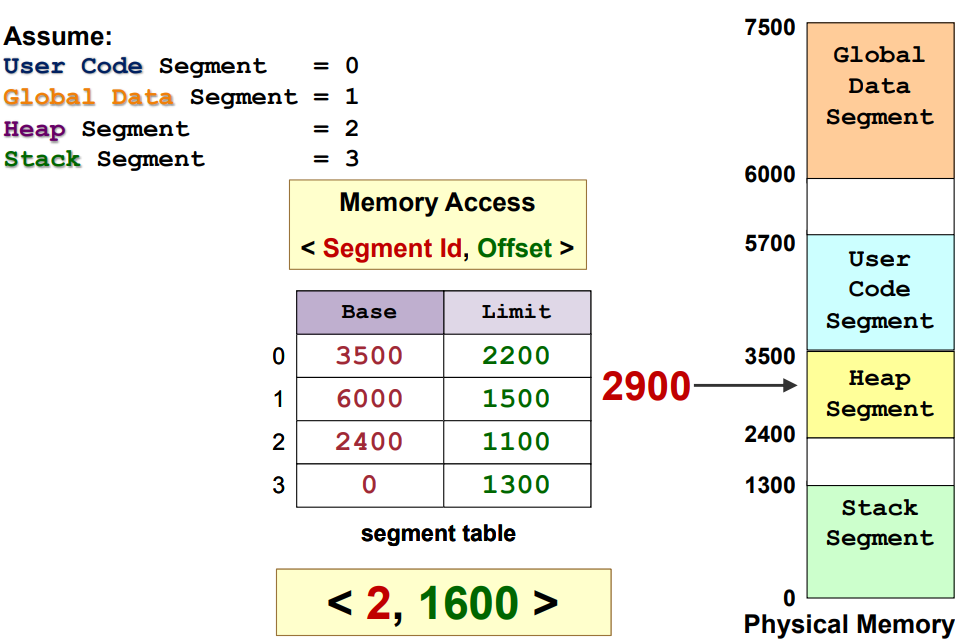
\includegraphics[width=8.5cm, height=4.5cm]{images/logicaladdresstranslation.png}
% 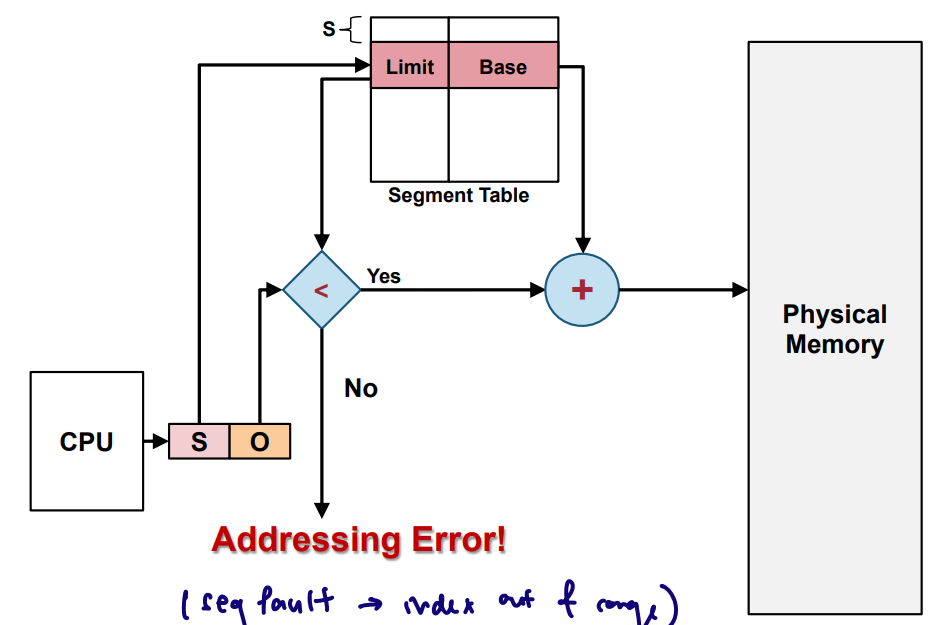
\includegraphics[width=8.5cm, height=4.5cm]{images/segmentationhardware.png}

\subsection*{Segmentation WITH Paging}
Each segment is now composed of several pages instead of a contiguous memory region, each segment has a page table.
Segment can grow by allocating new page then add to its page table (same for shrinking).

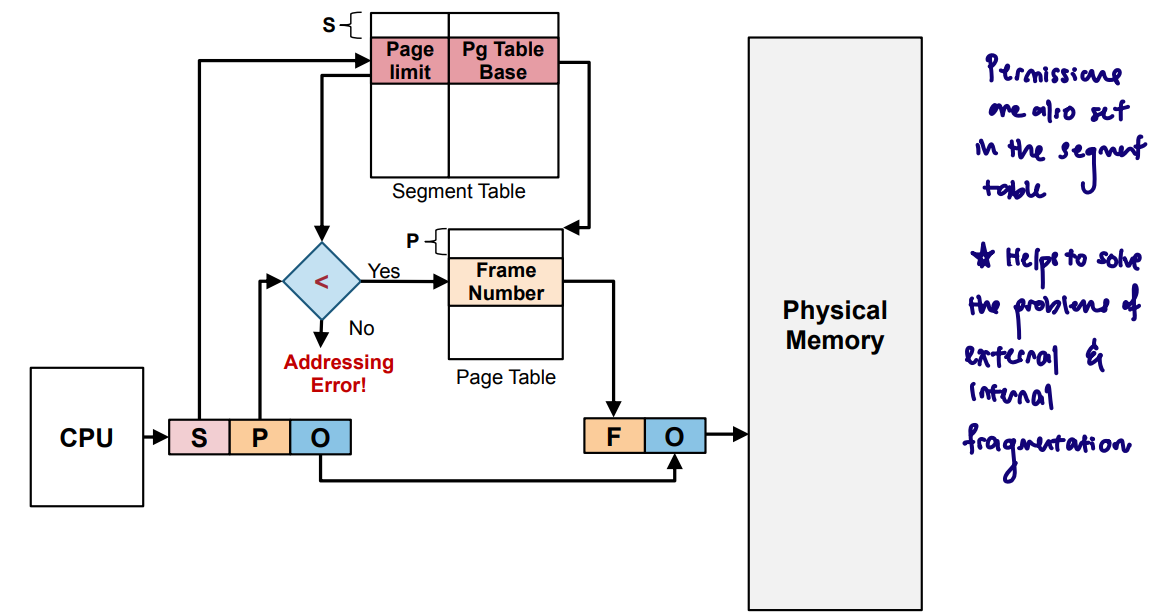
\includegraphics[width=8.5cm, height=4cm]{images/segmentationpaging.png}

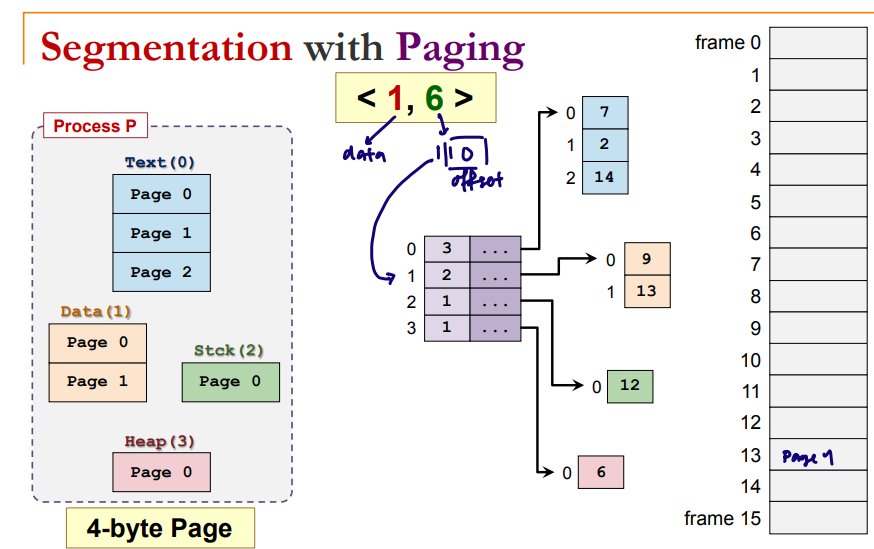
\includegraphics[width=8.5cm, height=4cm]{images/segmentationpaging2.png}

\subsection{\underline{Virtual Memory Management}}
Split the logical address space into small chunks, some reside in \textbf{physical memory}, others are stored in secondary storage.
\begin{enumerate}[topsep=0pt,noitemsep,wide=0pt, leftmargin=\dimexpr\labelwidth + 2\labelsep\relax]
    \item Secondary Storage (HDD/SDD) $>$ Physical Memory Capacity
    \item Some pages are access much more often than others
\end{enumerate}

\subsection*{Extended Paging System}
New addition to the paging scheme: 2 page types
\begin{itemize}[topsep=0pt,noitemsep,wide=0pt, leftmargin=\dimexpr\labelwidth + 2\labelsep\relax]
    \item \textbf{Memory Resident} (pages in physical memory)
    \item \textbf{Non-memory Resident} (pages in secondary storage)
    \item Use a \textit{resident bit} in the PTE $\rightarrow$ indicates whether the page is resident in memory
    \item CPU can only access memory resident pages $\rightarrow$ Page Fault when CPU tries to access non-memory resident page. OS brings non-memory resident page into physical memory
\end{itemize}

\subsubsection*{Access Page X: Steps}
\begin{enumerate}[topsep=0pt,noitemsep,wide=0pt, leftmargin=\dimexpr\labelwidth + 2\labelsep\relax]
    \item Check page table: Is page X memory resident? 
    \begin{itemize}[topsep=0pt,noitemsep,wide=0pt, leftmargin=\dimexpr\labelwidth + 2\labelsep\relax]
        \item Yes: Access physical memory location. No: raise exception
    \end{itemize}
    \item Page Fault: \textbf{OS takes control}
    \item Locate page X in secondary storage
    \item Load page X into physical memory and update page table
    \item Back to step 1, \textbf{\underline{re-execute same}} instruction
\end{enumerate}

% 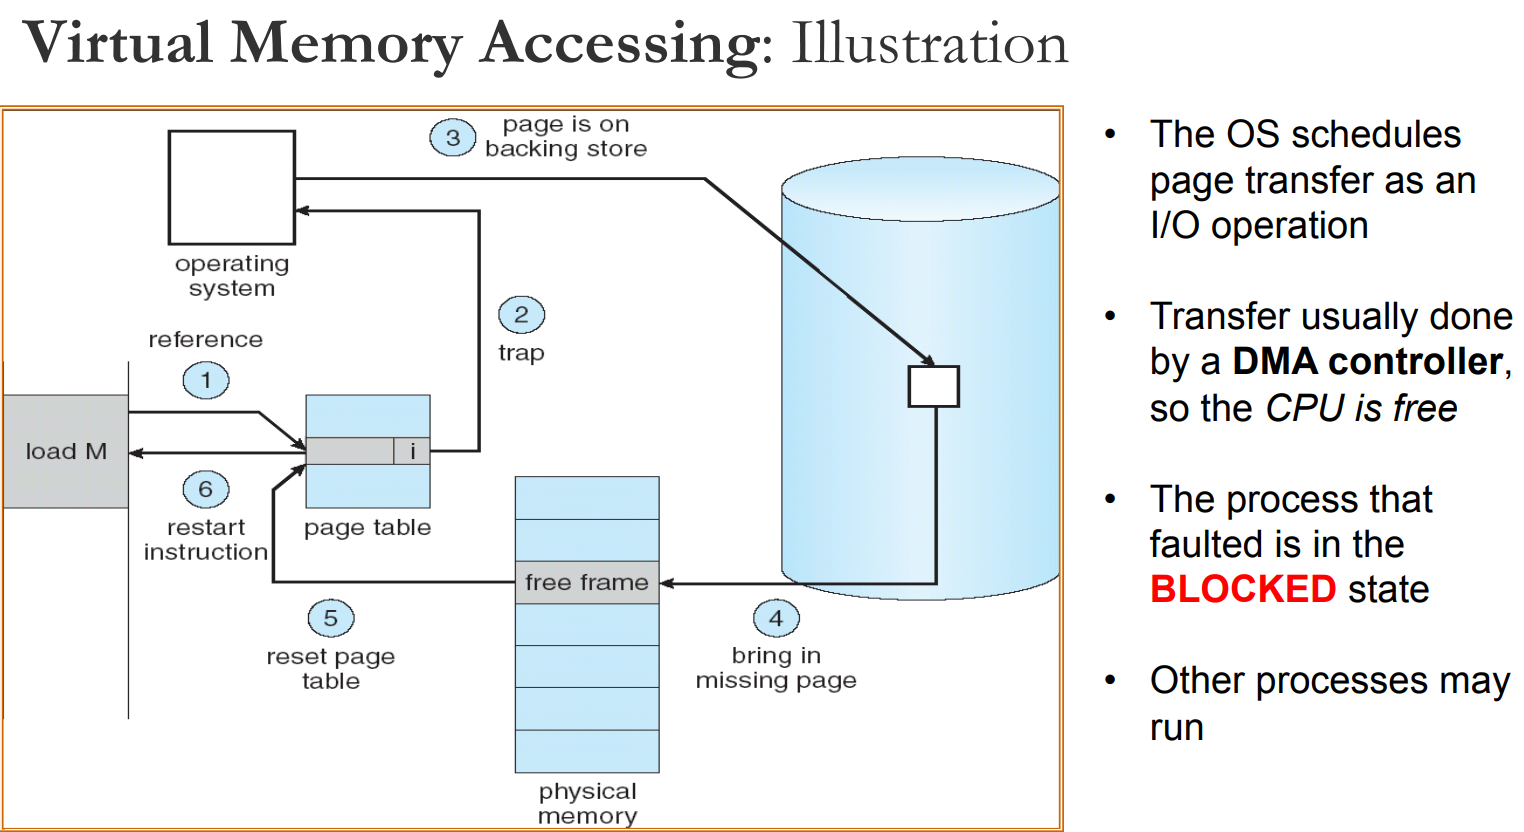
\includegraphics[width=8.5cm]{images/virtualmemoryaddressing.png}

\subsubsection*{Issues with Virtual Memory}
Secondary Storage access time $>$$>$ Physical memory access time (~5 orders of magnitude).
\begin{itemize}[topsep=0pt,noitemsep,wide=0pt, leftmargin=\dimexpr\labelwidth + 2\labelsep\relax]
    \item If memory access results in \textbf{page faults} often to load non-resident pages, slow system down, leading to thrashing
\end{itemize}

\subsection*{Locality Principles}
\begin{itemize}[topsep=0pt,noitemsep,wide=0pt, leftmargin=\dimexpr\labelwidth + 2\labelsep\relax]
    \item \textbf{Temporal:} Address used now \textbf{\textit{likely to be used again}}
    \item \textbf{Spatial:} Addresses close to address is likely to be used soon
\end{itemize}

\subsection*{Demand Paging || Laziness}
Processes start with no memory resident page, only allocate a page when there is a page fault.
\begin{itemize}[topsep=0pt,noitemsep,wide=0pt, leftmargin=\dimexpr\labelwidth + 2\labelsep\relax]
    \item \textbf{Pros}: Fast startup, small memory footprint
    \item \textbf{Cons}: Process appears slow initially due to many page faults, page faults might have a cascading effect on other processes (thrashing)
\end{itemize}

\subsection*{Page Table Structures}

\textbf{Direct Paging}
\colorbox{yellow!80}{% 
    $\# pages = \frac{2^{Virtual \ Address \ Space}}{Page \ Size}$ 
}  

Keep all entries in a single table AND page tables must be \textbf{contiguous} in OS memory.
\begin{itemize}[topsep=0pt,noitemsep,wide=0pt, leftmargin=\dimexpr\labelwidth + 2\labelsep\relax]
    \item With 2$^p$ pages in logical memory space: \textbf{p} bits to specify one unique page. 2$^p$ PTE with Physical Frame Number + Additional Information (valid, readonly etc)
    \item Virtual Address: 32 bits, Page Size = 4KB $\approx$ 2$^{12}$
    \item P = 32 - 12 = 20, size of PTE = 4 bytes, Page Table Size = 2$^{20}$ * 4 bytes = 4MB
    \item Even if page tables do not fit in a frame, OS must ensure that it is laid-out consecutively in its own memory.
\end{itemize}

\textbf{2-Level Paging | Paging the page table}
    \colorbox{yellow!80}{% 
        $Overhead = (\# PDE \times PTE \ Size) + (
            \# PT \times Page \ Size)$
    }
\begin{itemize}[topsep=0pt,noitemsep,wide=0pt, leftmargin=\dimexpr\labelwidth + 2\labelsep\relax]
    \item Split whole page table into regions, only a gew regions are used.
    \item As memory usage grows, new regions can be allocated.
    \item Directory is used to keep track of regions, analogues to the relationship between page tables and data pages.
    \item If original table has 2$^p$ entries,
    \begin{itemize}[topsep=0pt,noitemsep,wide=0pt, leftmargin=\dimexpr\labelwidth + 2\labelsep\relax]
        \item With 2$^M$ smaller pages tables, \textbf{M} bits used to uniquely identify one page table
        \item Each smaller page table contains 2$^{p - M}$ entries
    \end{itemize}
\end{itemize}
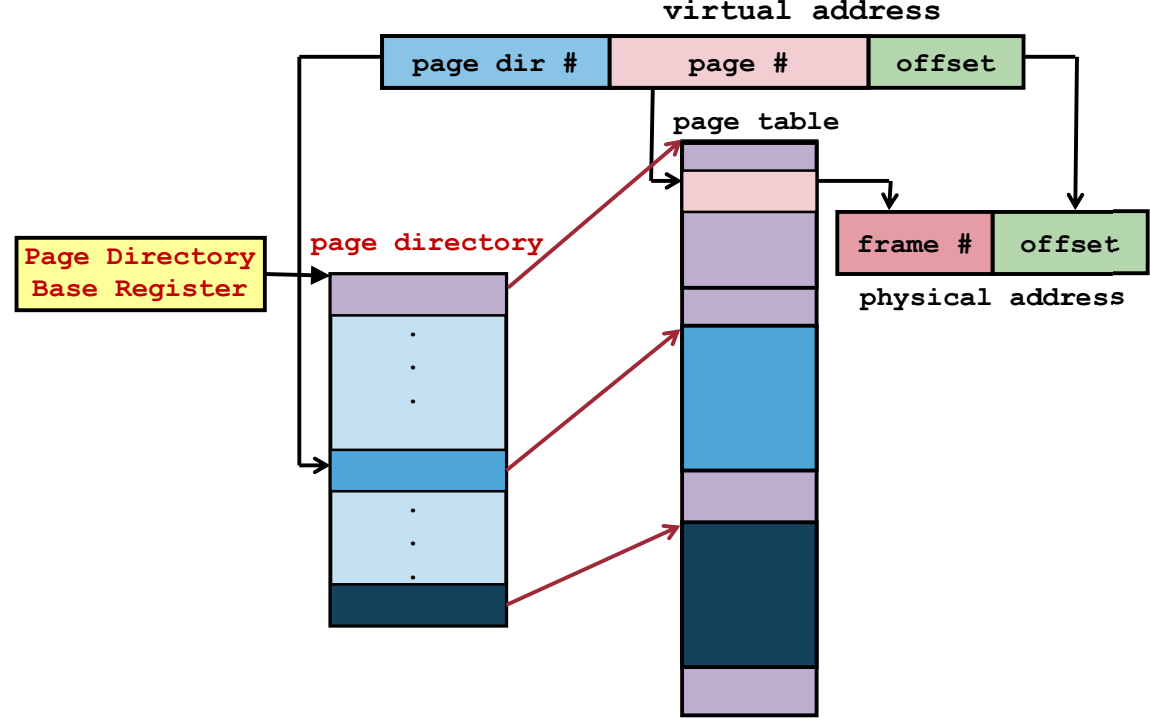
\includegraphics[width=4.2cm, height=3cm]{images/2levelpaging.png}
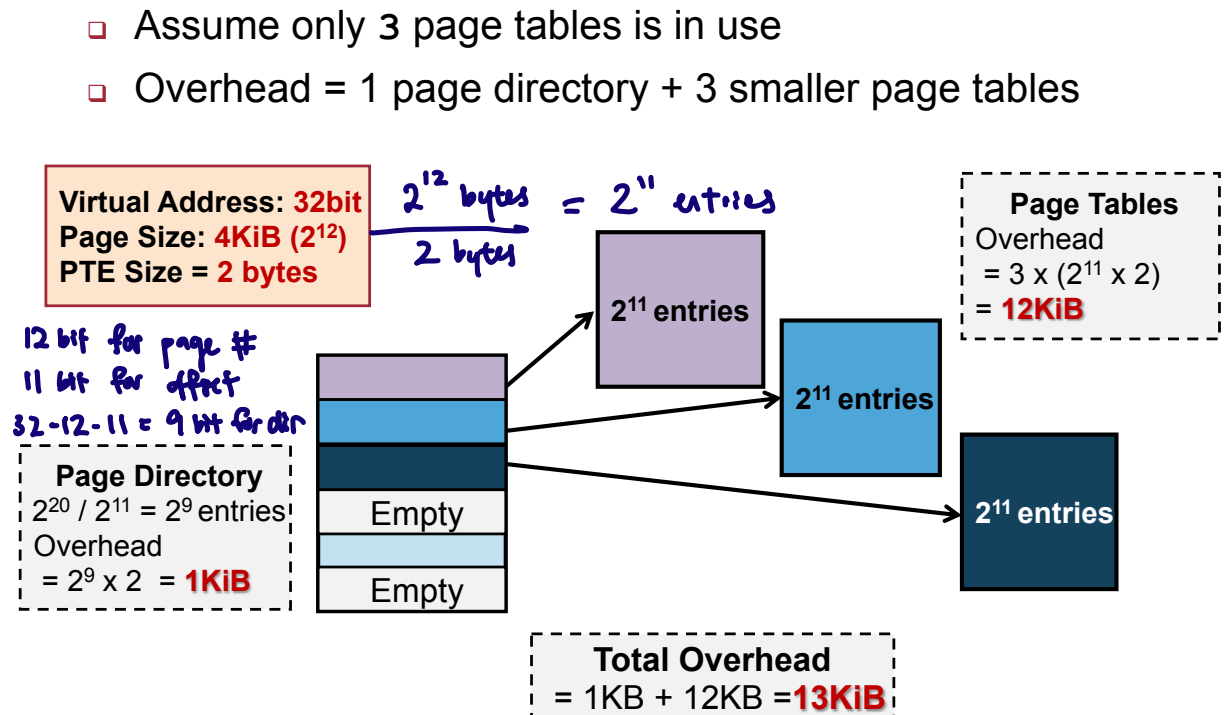
\includegraphics[width=4.2cm, height=3cm]{images/advantages2levelpaging.png}
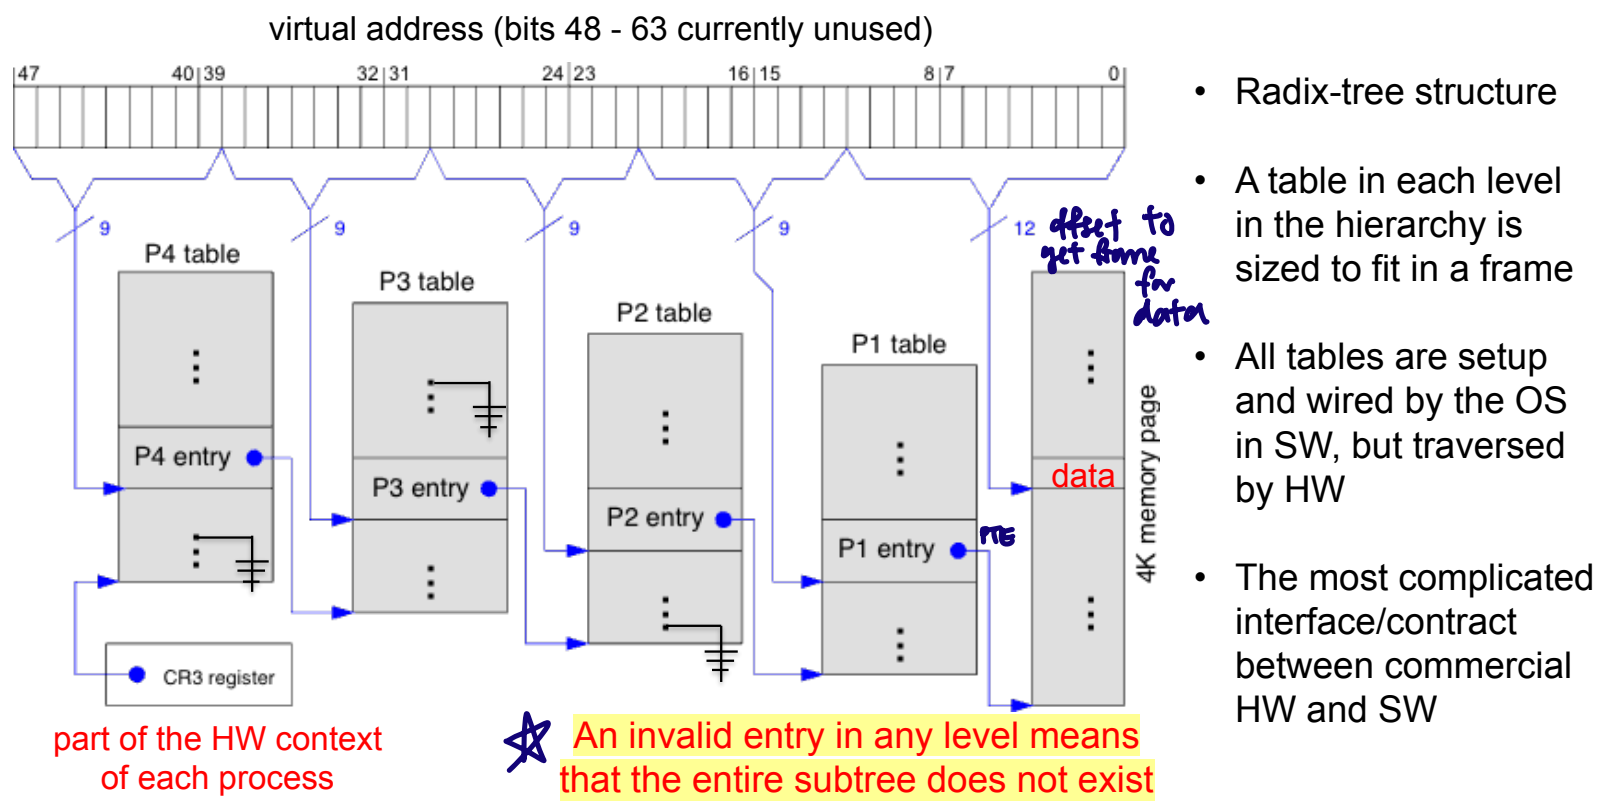
\includegraphics[width=8.5cm, height=3cm]{images/hierarchicalpagetable.png}

ADVANTAGES
\begin{itemize}[topsep=0pt,noitemsep,wide=0pt, leftmargin=\dimexpr\labelwidth + 2\labelsep\relax]
    \item Enables page tables to grow beyond size of frame, no need to be contiguous in OS memory
    \item Can have empty entries in the page directory
\end{itemize}


DISADVANTAGES
\begin{itemize}[topsep=0pt,noitemsep,wide=0pt, leftmargin=\dimexpr\labelwidth + 2\labelsep\relax]
    \item Requires 2 serialized memory address just to get frame number (1 dir, 1 page table)
    \item \textbf{TLB:} TLB hits eliminate page-table accesses, but TLB misses experience longer \textbf{page-table walks}.
    \item \textbf{MMU Caches}: additional hardware in modern processors
    \begin{itemize}[topsep=0pt,noitemsep,wide=0pt, leftmargin=\dimexpr\labelwidth + 2\labelsep\relax]
        \item tiny cache that caches frequent page directory entries, speed up page-table walk upon TLB miss.
        \item We do not want directory to kick out a PTE in TLB, thus use MMUs specifically for Directories.
    \end{itemize}
\end{itemize}


\textbf{Inverted Page Table}
\colorbox{yellow!80}{% 
    $\# \ frames = \frac{RAM \ size}{frame \ size}$
}

Keep a \textbf{single} mapping of physical frame to \verb|<pid, page#>|
\begin{itemize}[topsep=0pt,noitemsep,wide=0pt, leftmargin=\dimexpr\labelwidth + 2\labelsep\relax]
    \item pid = process id, page\# = logical page number in process
    \item page\# is not unqiue among processes
\end{itemize}
\textbf{Normal vs Inverted Page Table:} Entries ordered by page number vs frame number, lookup page X, simply access X$^{th}$ entry directly vs search whole table. 
ADVANTAGES: Huge saving, one table for all processes. DISADVANTAGES: Slow translation

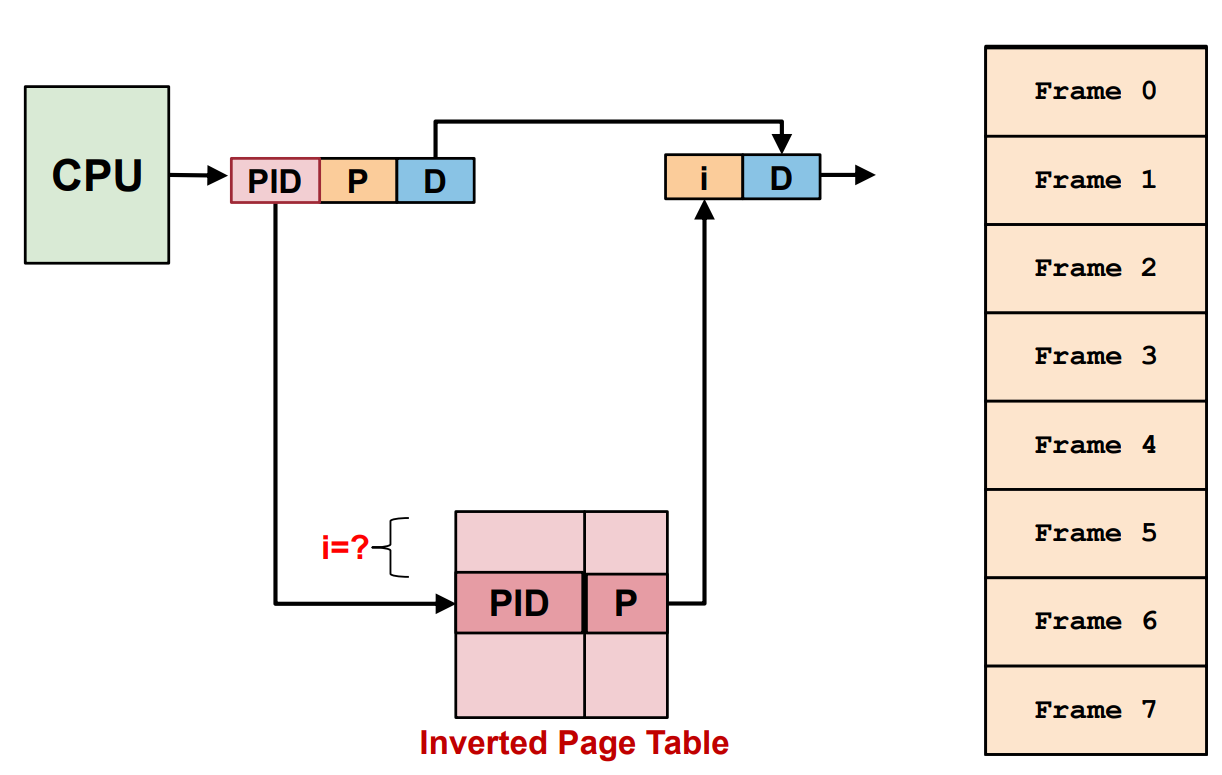
\includegraphics[width=8.5cm, height=3cm]{images/invertedpagetable.png}

\subsection*{Page Replacement Algorithms}
Which page should be replaced when needed. No free physical memory frame during a page fault, need to evict a memory page.
\begin{itemize}[topsep=0pt,noitemsep,wide=0pt, leftmargin=\dimexpr\labelwidth + 2\labelsep\relax]
    \item \textbf{Clean Page:} not modified $\rightarrow$ no need to write back
    \item \textbf{Dirty Page:} modified $\rightarrow$ need to write back
\end{itemize}

\subsubsection*{Evaluation}
A good algorithm should minimize the total number of \textbf{page faults} and be fast!
\textbf{Memory access time:}
\begin{equation*}
    T_{access} = (1-p) * T_{mem} + p * T_{page\_fault}
\end{equation*}
\begin{itemize}[topsep=0pt,noitemsep,wide=0pt, leftmargin=\dimexpr\labelwidth + 2\labelsep\relax]
    \item \verb|p| = probability of page fault
    \item \verb|T_mem| = access time for memory resident page
    \item \verb|T_pageFault| = access time if page fault occurs
    \item Since \verb|T_pageFault| $>$$>$ \verb|T_mem|, need to reduce \verb|p| to keep \verb|T_access| reasonable
\end{itemize}

\subsubsection*{1. Optimal Page Replacement}
Replace the page that \textbf{will not} be needed again for \textit{longest period of time}.
\textbf{Guarantees minimum} number of page faults. Not realizable as \textbf{need future knowledge} of memory references.
\underline{Closer to OPT, better algorithm.}

\subsubsection*{2. FIFO Page Replacement}
Memory pages evicted based on loading time $\rightarrow$ evict oldest memory page.
\begin{itemize}[topsep=0pt,noitemsep,wide=0pt, leftmargin=\dimexpr\labelwidth + 2\labelsep\relax]
    \item OS maintains queue of resident page numbers
    \item Remove the first page in queue if replacement is needed
    \item Update queue during page fault trap
    \item \textbf{Simple} to implement, no hardware support needed
\end{itemize}

Problems with FIFO:
\begin{itemize}[topsep=0pt,noitemsep,wide=0pt, leftmargin=\dimexpr\labelwidth + 2\labelsep\relax]
    \item Number of physical frame increases, number of page faults should increase
    \item Opposite behavior ($\uparrow$ frames $\rightarrow$ $\uparrow$ page faults)
    \begin{itemize}[topsep=0pt,noitemsep,wide=0pt, leftmargin=\dimexpr\labelwidth + 2\labelsep\relax]
        \item \textit{Belady's Anomaly}, does not exploit \textbf{temporal locality}
        \item Bad performance in practice
    \end{itemize}
\end{itemize}

\subsubsection*{3. \underline{L}east \underline{R}ecently \underline{U}sed (LRU)}
Make use of temporal locality, honour notion of \textit{recency}.
\begin{itemize}[topsep=0pt,noitemsep,wide=0pt, leftmargin=\dimexpr\labelwidth + 2\labelsep\relax]
    \item Replace page that has not been used in the longest time
    \item Aims to approximate OPT algorithm, predicting the future by mirroring the past
\end{itemize}

IMPLEMENTATION DETAILS
\begin{itemize}[topsep=0pt,noitemsep,wide=0pt, leftmargin=\dimexpr\labelwidth + 2\labelsep\relax]
    \item Need to keep track of `last access time', need substantial hardware support
    \item \textbf{A. Use a Counter}
    \begin{itemize}[topsep=0pt,noitemsep,wide=0pt, leftmargin=\dimexpr\labelwidth + 2\labelsep\relax]
        \item Logical time counter, increment on every memory reference
        \item Page table entry has time-of-use field, store time counter value whenever references occurs
        \item Replaced page with smallest time-of-use
        \item \textbf{Problems:} Need to search through all pages, time-of-use is forever increasing (overflow possible)
    \end{itemize}
    \item \textbf{B. Use a Stack}
    \begin{itemize}[topsep=0pt,noitemsep,wide=0pt, leftmargin=\dimexpr\labelwidth + 2\labelsep\relax]
        \item Maintain stack of page numbers, if \textbf{X} referenced, remove from stack and push to top.
        \item Replace the page at \textbf{bottom of stack}, no need to search through all entries
        \item \textbf{Problems:} Not a pure stack, since entries can be moved from anywhere in stack $\rightarrow$ hard to implement in hardware.
    \end{itemize}
\end{itemize}

\subsubsection*{3. Second-Chance Page Replacement | CLOCK}
Modified FIFO to give second change to pages accessed. Each PTE now maintains a \textit{referenced bit}.
\begin{itemize}[topsep=0pt,noitemsep,wide=0pt, leftmargin=\dimexpr\labelwidth + 2\labelsep\relax]
    \item 1 = Accessed since last reset, 0 = not accessed
    \item Algorithm: 
    \begin{enumerate}[topsep=0pt,noitemsep,wide=0pt, leftmargin=\dimexpr\labelwidth + 2\labelsep\relax]
        \item Oldest FIFO page selected
        \item If reference bit == 0 $\rightarrow$ page replaced, done.
        \item If reference bit == 1 $\rightarrow$ page skipped, given 2$^{nd}$ chance
        \begin{itemize}[topsep=0pt,noitemsep,wide=0pt, leftmargin=\dimexpr\labelwidth + 2\labelsep\relax]
            \item Reference bit cleared to 0, resets arrival time, page taken as newly loaded. Next FIFO page selected, go to Step 2
        \end{itemize}
    \end{enumerate}
    \item Becomes a FIFO algorithm when all page reference bits == 1
    \item Adds notion of recency, works well in practice
\end{itemize}

% 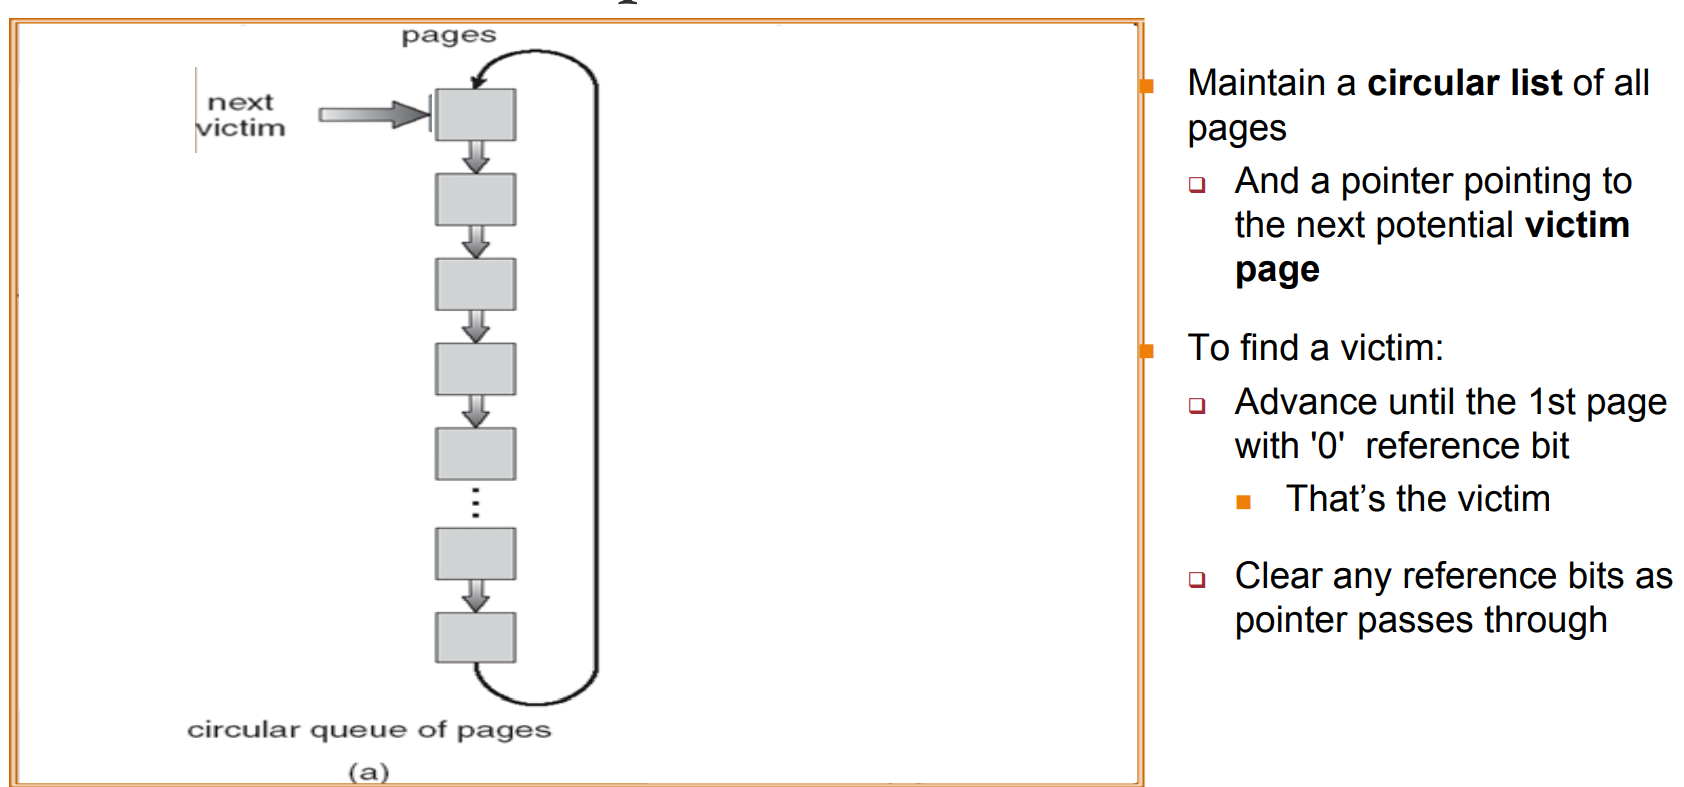
\includegraphics[width=8.5cm, height=3cm]{images/secondchance.png}

\subsection*{Page Table Structures}
\begin{itemize}[topsep=0pt,noitemsep,wide=0pt, leftmargin=\dimexpr\labelwidth + 2\labelsep\relax]
    \item \textbf{Equal Allocation:} Each process gets \verb|N| / \verb|M| frames
    \item \textbf{Proportional Allocation:}
    \begin{itemize}[topsep=0pt,noitemsep,wide=0pt, leftmargin=\dimexpr\labelwidth + 2\labelsep\relax]
        \item Processes different in size (memory usage)
        \item Let \verb|size_p| = size of process \verb|p|, \verb|size_total| = total size of all processes
        \item Each process get \verb|size_p|/\verb|size_total| * \verb|N| frames
    \end{itemize}
\end{itemize}

\textbf{Local replacement:} Victim page are selected among pages of the process that causes
page fault 
\begin{itemize}[topsep=0pt,noitemsep,wide=0pt, leftmargin=\dimexpr\labelwidth + 2\labelsep\relax]
    \item \textbf{Pros}: Number of frames allocated to a process remain constant
    $\rightarrow$ Performance is stable between multiple runs.
    \item \textbf{Cons}: If the frames allocated are not enough
    $\rightarrow$ hinder the progress of a process.
\end{itemize}

\textbf{Global replacement:} Victim page can be chosen among all physical frames:
$\rightarrow$ Process P can take a frame from Process Q by evicting Q's frame during replacement!

\begin{itemize}[topsep=0pt,noitemsep,wide=0pt, leftmargin=\dimexpr\labelwidth + 2\labelsep\relax]
    \item \textbf{Pros}: Allow self-adjustment between processes
    $\rightarrow$ Process that needs more frame can get from others that need less.
    \item \textbf{Cons}: Badly behaved processes can affect others. Number of frames allocated to a process can be different from run to run.
\end{itemize}

\subsubsection*{Thrashing}
Insufficient physical frames $\rightarrow$ Thrashing. Heavy I/O to bring non-resident pages into RAM.
\begin{itemize}[topsep=0pt,noitemsep,wide=0pt, leftmargin=\dimexpr\labelwidth + 2\labelsep\relax]
    \item Hard to find right number of frames:
    \begin{itemize}[topsep=0pt,noitemsep,wide=0pt, leftmargin=\dimexpr\labelwidth + 2\labelsep\relax]
        \item \textbf{Global used}: thrashing process `steals' page from other process, cause other process to thrash (cascading thrashing)
        \item \textbf{Local used}: thrashing limited to one process, but single process can use up I/O bandwidth, degrade performance of other processes
    \end{itemize}
\end{itemize}

\subsubsection*{Working Set Model}
Set of pages referenced by process is relatively constant in a period of time || known as \textbf{working set}.
As time passes, set of pages can change as different program phases require different data.

\begin{itemize}[topsep=0pt,noitemsep,wide=0pt, leftmargin=\dimexpr\labelwidth + 2\labelsep\relax]
    \item Working set stable and well-defined, rare for page faults
    \item When transitioning to new working set, many page faults for new set of pages
    \item Defines a \textbf{Working Set Window} $\triangle$ $\rightarrow$ an interval of time
    \item \verb|W(t,| $\triangle$ \verb|)| = active pages in interval time \verb|t|
    \item Allocate enough frames for pages in \verb|W(t,| $\triangle$ \verb|)| to reduce possibility of page fault.
    \item Too small, miss pages in current working set, Too big, contain page in different working set
\end{itemize}


\begin{itemize}[topsep=0pt,noitemsep,wide=0pt, leftmargin=\dimexpr\labelwidth + 2\labelsep\relax]
    \item Assume $\triangle$ = an interval of 5 memory references
    \item \verb|W(t1,| $\triangle$ \verb|) = {1,2,5,6,7}| (5 frames needed)
    \item \verb|W(t2,| $\triangle$ \verb|) = {3,4}| (2 frames needed)
\end{itemize}
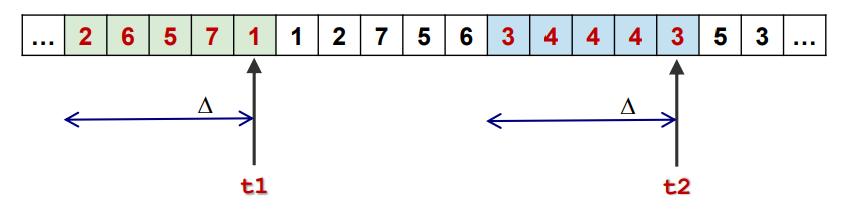
\includegraphics[width=6.5cm, height=1.2cm]{images/workingsetmodel2.png}

\subsection*{\underline{File System Introduction}}
It is an abstraction on top of physical media, high-level resource management scheme. 
It must ensure protection between processes and users, and be shared between processes and users.

\begin{itemize}[topsep=0pt,noitemsep,wide=0pt, leftmargin=\dimexpr\labelwidth + 2\labelsep\relax]
    \item \textbf{Self-Contained:} Information stored on media enough to describe entire organisation $\rightarrow$ plug and play
    \item \textbf{Persistent:} Beyond the lifetime of OS and processes
    \item \textbf{Efficient:} Provides good manangement of free and unused space + minimum overhead of bookkeeping information
\end{itemize}

\subsubsection*{File Overview}
\textbf{File Name:} Different FS have different naming rules: length of file name, case sensitivity, allow special symbols and file extensions.

\textbf{File Type:}
\begin{enumerate}[topsep=0pt,noitemsep,wide=0pt, leftmargin=\dimexpr\labelwidth + 2\labelsep\relax]
    \item \textbf{Regular files:} contains user info (ASCII/binary files)
    \begin{itemize}[topsep=0pt,noitemsep,wide=0pt, leftmargin=\dimexpr\labelwidth + 2\labelsep\relax]
        \item \textit{ASCII:} text file, programming source code
        \item \textit{Binary files:} executable, Java \verb|.class| files, \verb|.pdf| file, \verb|png| etc. Have a predefined internal structure that can be pprocess by a specific program (JVM for Java \verb|.class|)
    \end{itemize}
    \item \textbf{Directories:} system files for FS structure
    \item \textbf{Special files:} character/block oriented
    \item Distinguished by \textbf{file extension} (Windows $\rightarrow$ \verb|XXX.docx| Word Document) OR \textbf{embedded information} (Unix),
    usually stored at beginning of file $\rightarrow$ magic number
\end{enumerate}

\textbf{File Protection:} \\
Accessing information: Read/Write/Execute/Append/Delete/List
\begin{itemize}[topsep=0pt,noitemsep,wide=0pt, leftmargin=\dimexpr\labelwidth + 2\labelsep\relax]
    \item Permission Bits
    \begin{itemize}[topsep=0pt,noitemsep,wide=0pt, leftmargin=\dimexpr\labelwidth + 2\labelsep\relax]
        \item \textbf{Owner:} User who created the file
        \item \textbf{Group:} Set of users who need similar access to a file
        \item \textbf{Universe:} All other users in the system
    \end{itemize}
    \item Access Control List: Minimal ACL (same as permission bits) or Extended ACL (added named users/group)
\end{itemize}

\textbf{File Structure}
\begin{itemize}[topsep=0pt,noitemsep,wide=0pt, leftmargin=\dimexpr\labelwidth + 2\labelsep\relax]
    \item \textbf{Array of bytes}: each byte has unique offset from the file start
    \item \textbf{Fixed length records:} Array of records can grow/shrink, can jump to any record easily.
    \item \textbf{Variable length records:} Flexible but hard to locate.
\end{itemize}

\textbf{Access Methods}
\begin{itemize}[topsep=0pt,noitemsep,wide=0pt, leftmargin=\dimexpr\labelwidth + 2\labelsep\relax]
    \item \textbf{Sequential Access:} Data read in order, start from beginning but cannot skip can rewound
    \item \textbf{Random Access:} Read in any order, \verb|Read( Offset )|, \verb|Seek( Offset )| to move to new location in file
    \item \textbf{Direct Access:} Used for file that contains fixed-length records, allow random access to any record directly. Useful when there is large amount of records.
\end{itemize}

\textbf{File Information:} \\ 
\textbf{Operations:} Create, Open, Read, Write, Repositioning (seek), Truncate
Information kept for an open file
\begin{itemize}[topsep=0pt,noitemsep,wide=0pt, leftmargin=\dimexpr\labelwidth + 2\labelsep\relax]
    \item \textbf{File pointer:} keep track of current position within file
    \item \textbf{File descriptor:} unique identifier of the file
    \item \textbf{Disk Location:} actual file location on disk
    \item \textbf{Open Count/Reference count:} how many processes has this file open (used to determine when can remove from table.)
\end{itemize}

\begin{itemize}[topsep=0pt,noitemsep,wide=0pt, leftmargin=\dimexpr\labelwidth + 2\labelsep\relax]
    \item \textbf{Per-process open-file table:}
    \begin{itemize}[topsep=0pt,noitemsep,wide=0pt, leftmargin=\dimexpr\labelwidth + 2\labelsep\relax]
        \item Keep track of open files for a process
        \item Each entry points to the \textbf{system-wide open-file table} entries $\rightarrow$ if \verb|open()| is called twice, there will be 2 seperate \verb|fd|
    \end{itemize}
    \item \textbf{System-wide open-file table:}
    \begin{itemize}[topsep=0pt,noitemsep,wide=0pt, leftmargin=\dimexpr\labelwidth + 2\labelsep\relax]
        \item Keep track of all open files in the system
        \item Each entry points to a \textbf{V-node} entry
    \end{itemize}
    \item \textbf{System-wide V-node(virtual node) table:}
    \begin{itemize}[topsep=0pt,noitemsep,wide=0pt, leftmargin=\dimexpr\labelwidth + 2\labelsep\relax]
        \item Link with the file on physical drive
        \item Contains the information about the physical location of the file
    \end{itemize}
\end{itemize}

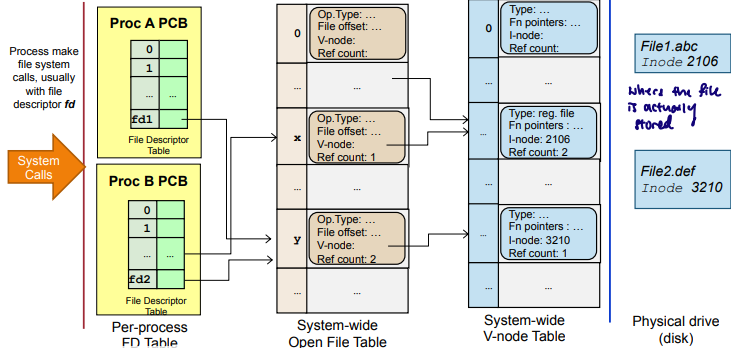
\includegraphics[width=8.5cm, height=4cm]{images/fileoperations.png}
\begin{itemize}[topsep=0pt,noitemsep,wide=0pt, leftmargin=\dimexpr\labelwidth + 2\labelsep\relax]
    \item V-Node table consists of Files that are \textbf{open}, in RAM
    \item I-Node is in harddisk, that consists of data of ALL files.
\end{itemize}


File opened twice from 2 processes $\mid$ 2 using same entry \verb|fork()|
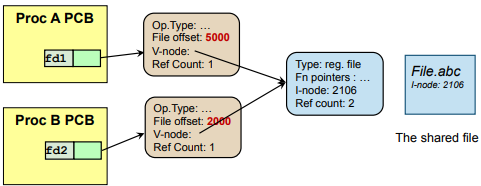
\includegraphics[width=4.2cm, height=2cm]{images/processsharingcase1.png}
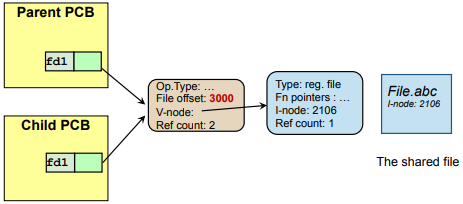
\includegraphics[width=4.2cm, height=2cm]{images/processsharingcase2.png}

\subsection*{Directories}
\subsubsection*{Tree-Structured}
\begin{itemize}[topsep=0pt,noitemsep,wide=0pt, leftmargin=\dimexpr\labelwidth + 2\labelsep\relax]
    \item Directories recursively embedded in other directories
    \item \textbf{Absolute Path:} Dir names followed from root of tree + final file, path from root dir to file
    \item \textbf{Relative Path:} Dir names from the current working directory (CWD), can be set explicitly or implcitly changed by moving into a new dir under shell prompt
\end{itemize}

% \subsubsection*{DAG}
% \begin{itemize}[topsep=0pt,noitemsep,wide=0pt, leftmargin=\dimexpr\labelwidth + 2\labelsep\relax]
%     \item If file can be shared, only one copy of actual content. 
%     \item `Appears' in multiple dirs with different path name, 2 file names refer to the same file content
%     \item Implemeneted as a \textit{hard link} in Unix.
% \end{itemize}

\cprotect\subsubsection{DAG || Unix Hard Link \verb|ln|}
\begin{itemize}[topsep=0pt,noitemsep,wide=0pt, leftmargin=\dimexpr\labelwidth + 2\labelsep\relax]
    \item Dir \verb|A| owns file \verb|F|, Dir \verb|B| wants to share \verb|F|
    \item \verb|A| and \verb|B| has separate pointers point to actual file F in disk
    \item \textbf{Pros:} Low overhead, only pointers added in directory.
    \item \textbf{Cons:} Deletion problems, if use reference count, if count $>$ 1 do not delete.
\end{itemize}

% \subsubsection*{General Graph}
% \begin{itemize}[topsep=0pt,noitemsep,wide=0pt, leftmargin=\dimexpr\labelwidth + 2\labelsep\relax]
%     \item Hard to traverse, need to prevent infinite looping
%     \item Hard to determine when to remove a file/dir
%     \item In Unix, \textit{Symbolic link} is allowed to link directory, general graph \textbf{can be created}
% \end{itemize}

\cprotect\subsubsection{DAG || Unix Sym/Soft Link \verb|ln -s|}
\begin{itemize}[topsep=0pt,noitemsep,wide=0pt, leftmargin=\dimexpr\labelwidth + 2\labelsep\relax]
    \item Symbolic link is a \textbf{special link file} \verb|G|, contains path name of \verb|F|
    \item When \verb|G| accessed: find out where is \verb|F|, then access \verb|F|
    \item \textbf{Pros:} Simple deletion, if symbolic link deleted (\verb|G| deleted), \verb|F| not deleted. If linked file
    is deleted: \verb|F| is gone, \verb|G| remains but is dangling link.   
    \item \textbf{Cons:} Larger overhead, special link file take up space.  
\end{itemize}

\subsection*{\underline{File System Implementation}}
General \textbf{Disk Structure} is a 1D array of logicial blocks (smallest accessible unit).
Logical block is mapped into disk sector(s), hardware dependent.

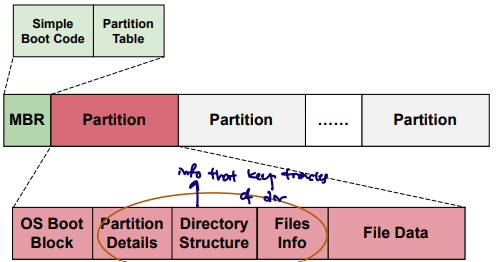
\includegraphics[width=8.5cm, height=3cm]{images/genericdiskorg.png}
\begin{itemize}[topsep=0pt,noitemsep,wide=0pt, leftmargin=\dimexpr\labelwidth + 2\labelsep\relax]
    \item \textbf{Master Boot Record} at sector 0 with partition table
    \item Each partition can contain an indepedent file system
    \item File system generally contains the following:
\end{itemize}

\subsection*{Implementing File}
Within the \verb|Files Info| + \verb|Files Data| in Disk Organisation.

\subsubsection*{File Block Allocation: \textit{Contiguous}}
Allocate consecutive disk blocks to files
\begin{minipage}[c]{0.63\linewidth}
    \begin{itemize}[topsep=0pt,noitemsep,wide=0pt, leftmargin=\dimexpr\labelwidth + 2\labelsep\relax]
        \item \textbf{Pros:} Simple \& fast access (only need to seek first block)
        \item \textbf{Cons:} External Frag. File size needs to be specified in advance.
    \end{itemize}
\end{minipage} % no space if you would like to put them side by side
\hspace{0.02\textwidth}%
\begin{minipage}[c]{0.2\linewidth}
        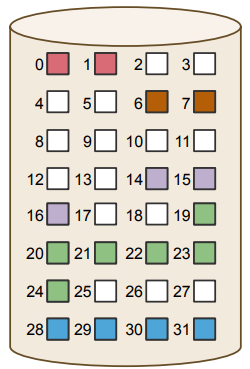
\includegraphics[width=1.8cm, height=2.2cm]{images/contiguous.png}    
\end{minipage}

\subsubsection*{File Block Allocation: \textit{Linked List}}
Keep linked list of disk blocks. Each disk block stores next disk block number (act as \textbf{pointer}) + actual file data.
File information stores first and last disk block number.
\begin{minipage}[c]{0.63\linewidth}
    \begin{itemize}[topsep=0pt,noitemsep,wide=0pt, leftmargin=\dimexpr\labelwidth + 2\labelsep\relax]
        \item \textbf{Pros:} Solve fragmentation problem.
        \item \textbf{Cons:} Random file access is very slow. Part of disk block used for pointer $\rightarrow$ what if one of the pointers is wrong (less reliable)
    \end{itemize}
\end{minipage} % no space if you would like to put them side by side
\hspace{0.02\textwidth}%
\begin{minipage}[c]{0.2\linewidth}
        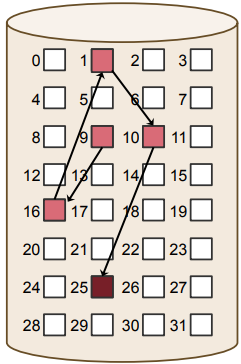
\includegraphics[width=1.8cm, height=2.2cm]{images/linkedlistfile.png}    
\end{minipage}



\subsubsection*{File Block Allocation: \textit{File Allocation Table (FAT)}}
All block pointers in a single table, FAT in memory all the time. 
\begin{minipage}[c]{0.43\linewidth}
    \begin{itemize}[topsep=0pt,noitemsep,wide=0pt, leftmargin=\dimexpr\labelwidth + 2\labelsep\relax]
        \item \textbf{Pros:} Faster than random access, linked list traversal now takes place in memory.
        \item \textbf{Cons:} FAT keeps track of \textbf{all disk blocks} in partition. Can be huge when disk is large, expensive overhead.
    \end{itemize}
\end{minipage} % no space if you would like to put them side by side
\hspace{0.02\textwidth}%
\begin{minipage}[c]{0.4\linewidth}
        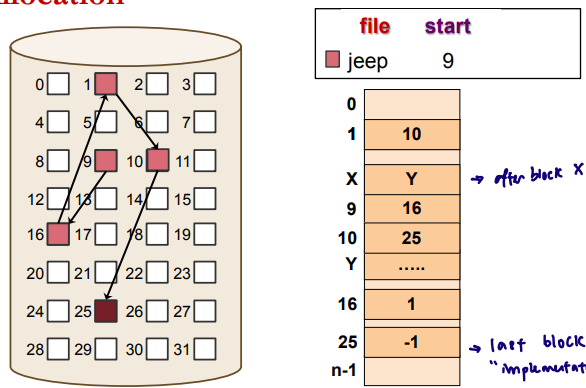
\includegraphics[width=4.5cm, height=3.5cm]{images/fatallocation.png}    
\end{minipage}



\subsubsection*{File Block Allocation: \textit{Indexed Allocation}}
Instead of keeping track of every file in system, maintain blocks for each file. Each file has \textbf{index block}.
Index block is an array of disk block addresses, \verb|IndexBlock[N]| == N$^{th}$ block address.

\begin{minipage}[c]{0.4\linewidth}
    \begin{itemize}[topsep=0pt,noitemsep,wide=0pt, leftmargin=\dimexpr\labelwidth + 2\labelsep\relax]
        \item \textbf{Pros:} Less memory overhead, only index block of opened file needs to be in memory. Fast direct access.
        \item \textbf{Cons:} Limited maximum file size and Index block overhead. Max number of blocks == Number of index block entries
    \end{itemize}
\end{minipage} % no space if you would like to put them side by side
\hspace{0.02\textwidth}%
\begin{minipage}[c]{0.43\linewidth}
        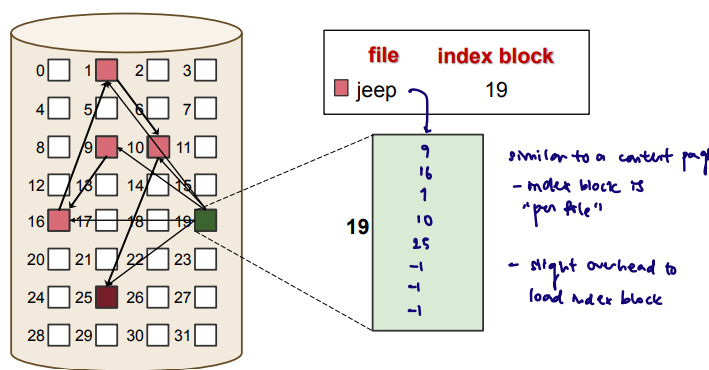
\includegraphics[width=5cm, height=3.5cm]{images/indexedallocation.png}    
\end{minipage}

\subsubsection*{VARIATIONS of indexed block allocation}
\begin{itemize}[topsep=0pt,noitemsep,wide=0pt, leftmargin=\dimexpr\labelwidth + 2\labelsep\relax]
    \item \textbf{Linked:} Linkedlist of index nodes, expensive traversal cost
    \item \textbf{Multi-level Index:} Similar idea to multi-level paging, can be generalized to any number of levels
    \item \textbf{Combined scheme:} Combination of direct indexing and multi-level index scheme, fast access for small files but can handle large files
\end{itemize}

\subsection*{Free Space Management}
Within \verb|Partition Details| of Disk Organisation. To perform file allocation,
we need to know which disk blocks are free.
\begin{itemize}[topsep=0pt,noitemsep,wide=0pt, leftmargin=\dimexpr\labelwidth + 2\labelsep\relax]
    \item \textbf{Allocation:} Remove free disk blocks from free space list. (when file created/enlarged)
    \item \textbf{Free:} Add free disk blocks to free space list (when file deleted/truncated)
\end{itemize}

\subsubsection*{Bitmap}
Each disk block represented by 1 bit: \verb|0 1 0 1 1 1 0 1 0 1 1| \\
Occupied: 0, 2, 6, 7, 9 ... | Free: 1, 3, 4, 5, 8, 10, 11 ...
\begin{itemize}[topsep=0pt,noitemsep,wide=0pt, leftmargin=\dimexpr\labelwidth + 2\labelsep\relax]
    \item \textbf{Pros:} Good set of manipulations
    \item \textbf{Cons:} Need to be kept in memory for efficiency
\end{itemize}

\subsubsection*{LinkedList}
Use linkedlist of blocks, each disk block contains (1) number of free disk blocks OR (2) pointer to the next free space disk block.
\begin{minipage}[c]{0.6\linewidth}
    \begin{itemize}[topsep=0pt,noitemsep,wide=0pt, leftmargin=\dimexpr\labelwidth + 2\labelsep\relax]
        \item \textbf{Pros:} Easy to locate free block, only first pointer needs to be in memory. (other blocks cached)
        \item \textbf{Cons:} High overhead.
    \end{itemize}
\end{minipage} % no space if you would like to put them side by side
\hspace{0.02\textwidth}%
\begin{minipage}[c]{0.23\linewidth}
        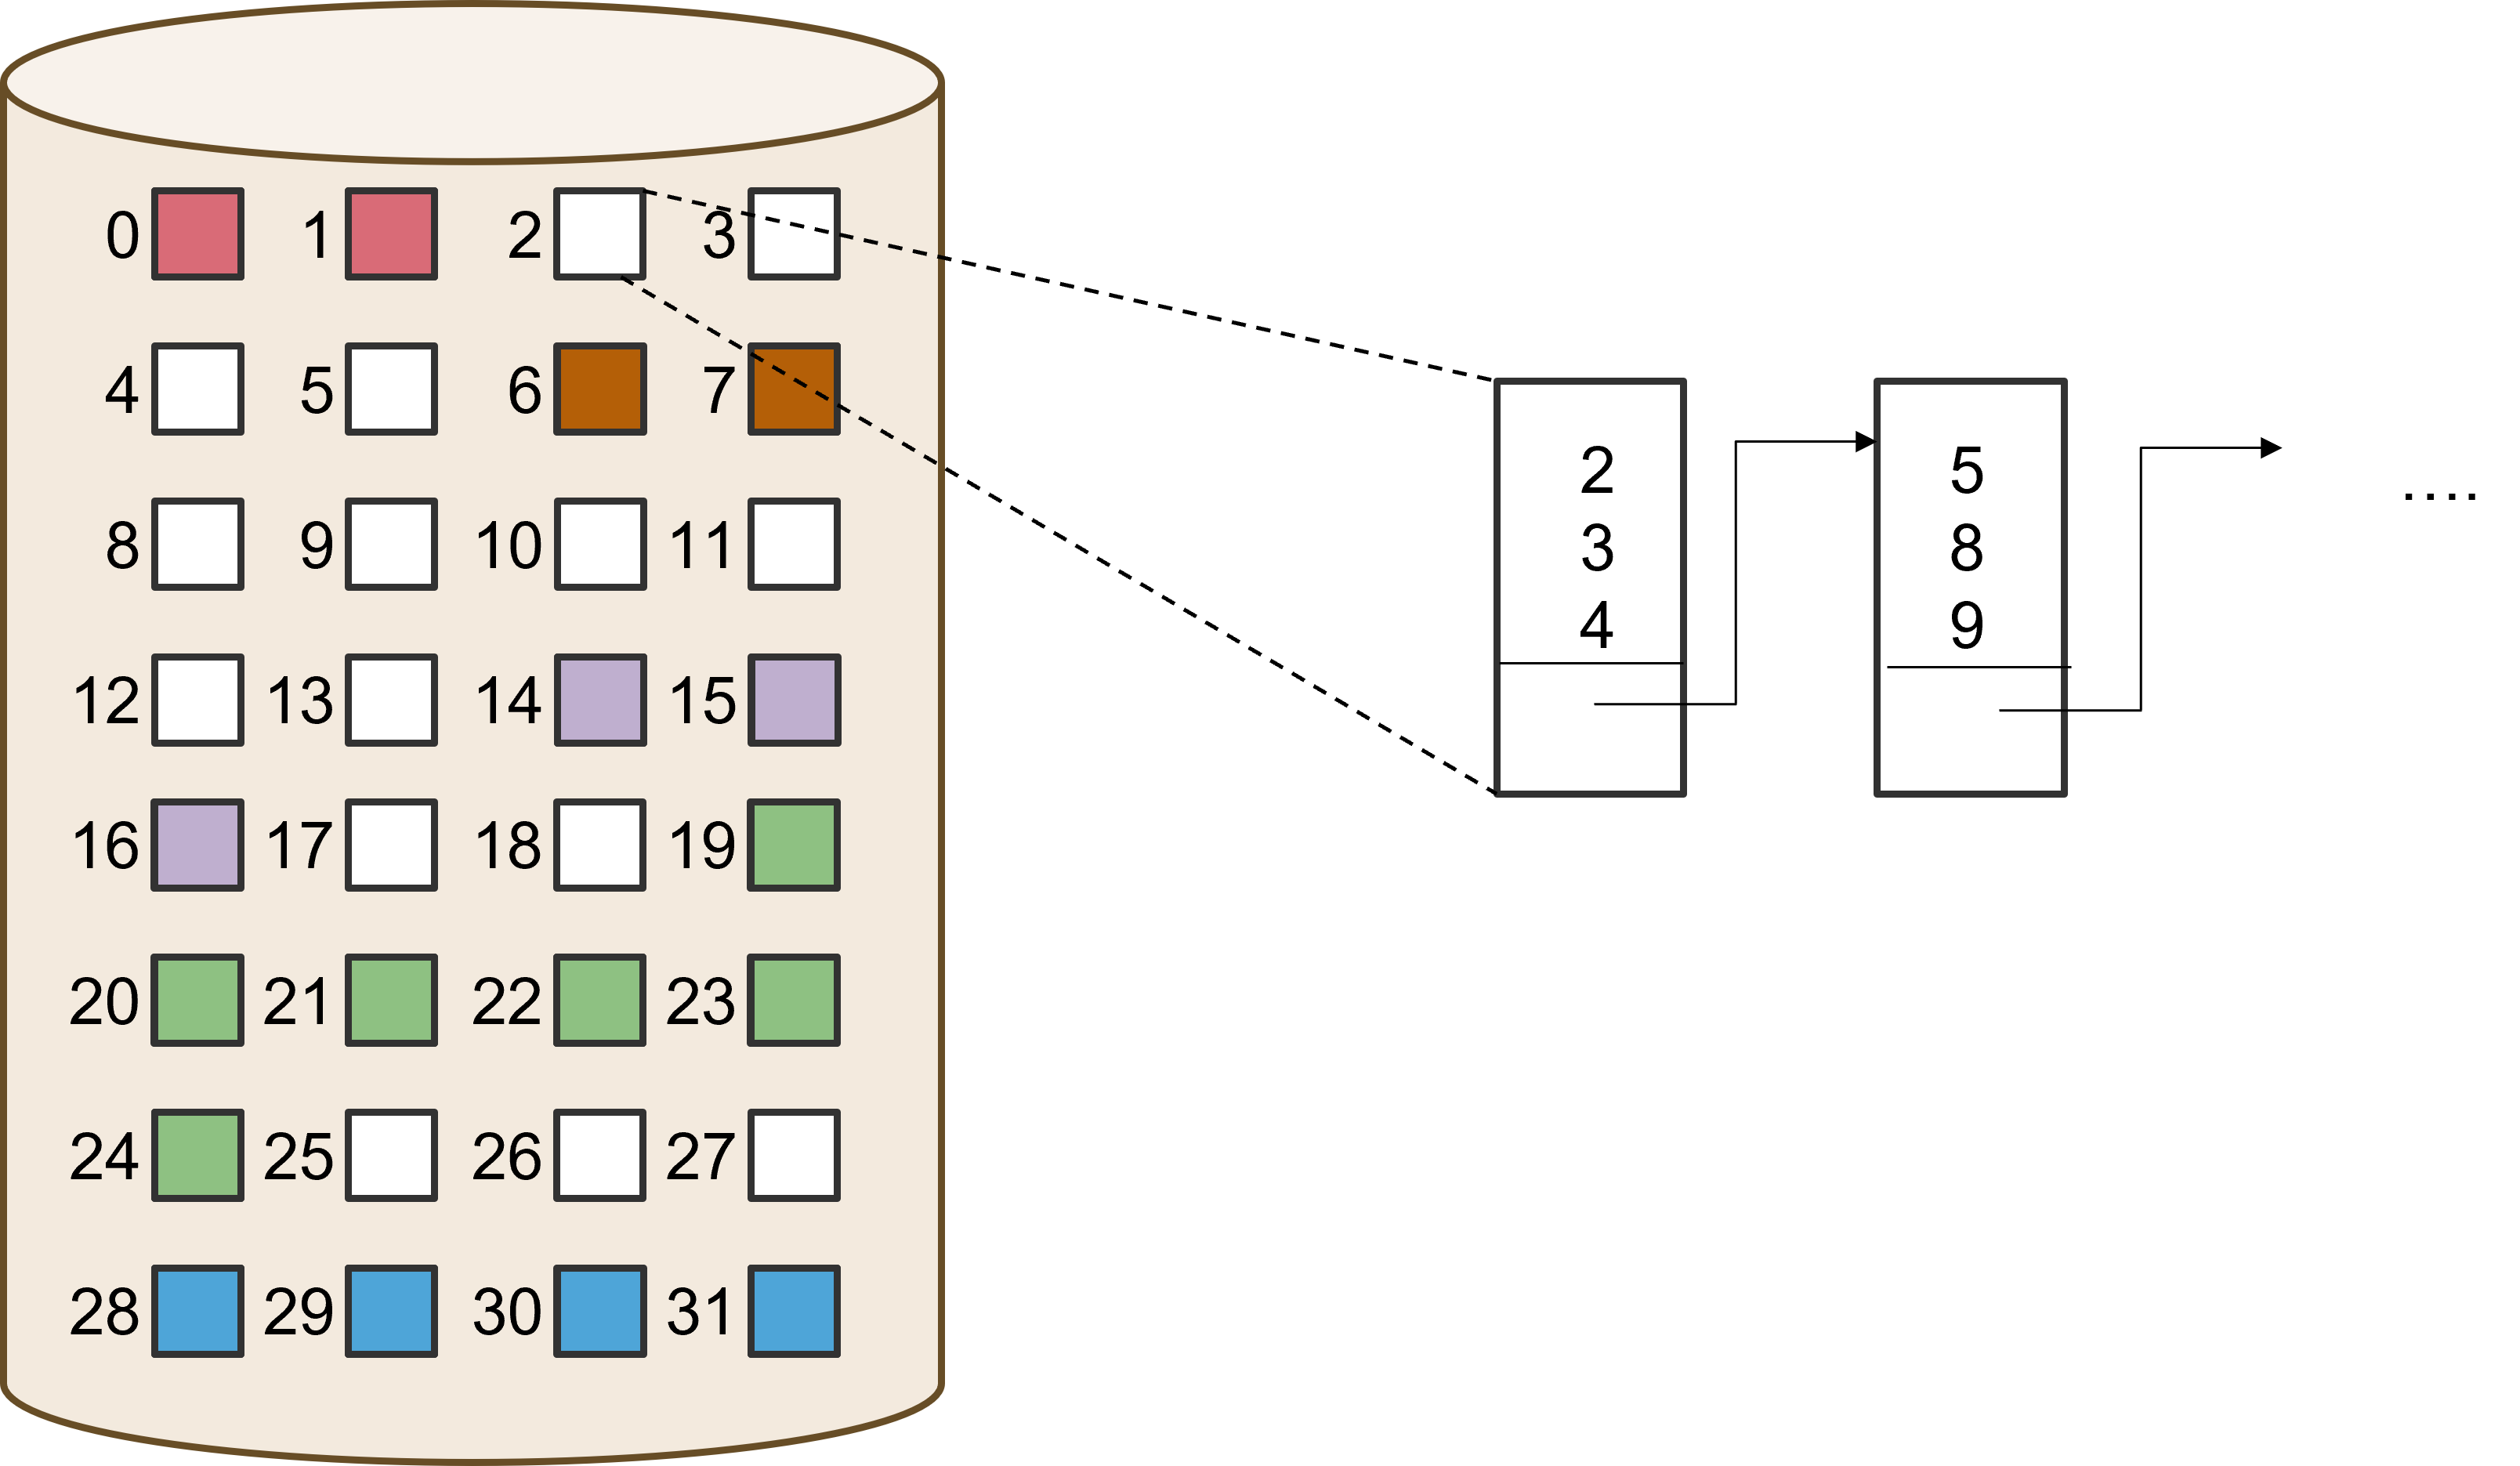
\includegraphics[width=3.5cm, height=2cm]{images/linkedlistfree.png}    
\end{minipage}

\subsection*{Directory Structure}
Within \verb|Directory Structure| of Disk Organisation. Keeps tracks of files in directory and map file name to file information.
\verb|open()| operation is to locate file info using \verb|pathname| + \verb|file name|
\begin{itemize}[topsep=0pt,noitemsep,wide=0pt, leftmargin=\dimexpr\labelwidth + 2\labelsep\relax]
    \item Given full path name, need to recursively search directories along path to arrive at file information
    \item Sub-directories stored as file entry with special type
\end{itemize}

\subsubsection*{Linear List}
Each entry in list represents file. Stores file name (minimally) and file metadata $\rightarrow$ \textbf{file information} / \textbf{pointer} to file information.
\\ File located by \textbf{linear search}, inefficient for larger directories / deep traversals. (use cache to remember recent searches).

\subsubsection*{Hash Table}
Each directory contains hash table of size \verb|N|. To locate, filename hashed into index \verb|K| from \verb|0| to \verb|N-1|. \verb|HashTable[K]| inspected to match file name.
(usually chained collision resolution used.)
\begin{itemize}[topsep=0pt,noitemsep,wide=0pt, leftmargin=\dimexpr\labelwidth + 2\labelsep\relax]
    \item \textbf{Pros:} Fast lookup, \textit{O(1)} versus \textit{O(n)} in linear list.
    \item \textbf{Cons:} Limited size Hash table \& depend on good hash functions.
\end{itemize}

\subsubsection*{File Information}
File info consists of file name and other metadata + disk blocks information.
\begin{itemize}[topsep=0pt,noitemsep,wide=0pt, leftmargin=\dimexpr\labelwidth + 2\labelsep\relax]
    \item Store everything in directory entry
    \item Store only file name, point to DS for other information
\end{itemize}

\subsection*{Microsoft FAT File System}
\subsubsection*{File Data + FAT Implementation}
\begin{itemize}[topsep=0pt,noitemsep,wide=0pt, leftmargin=\dimexpr\labelwidth + 2\labelsep\relax]
    \item File data allocated to some data blocks / block clusters
    \item Allocation info kept as \textbf{linked list}, data block pointers kept separately in FAT
    \item One entry per data block/cluster. Store disk block info. Os will cache in RAM to facilliate linkedlist traversal
\end{itemize}

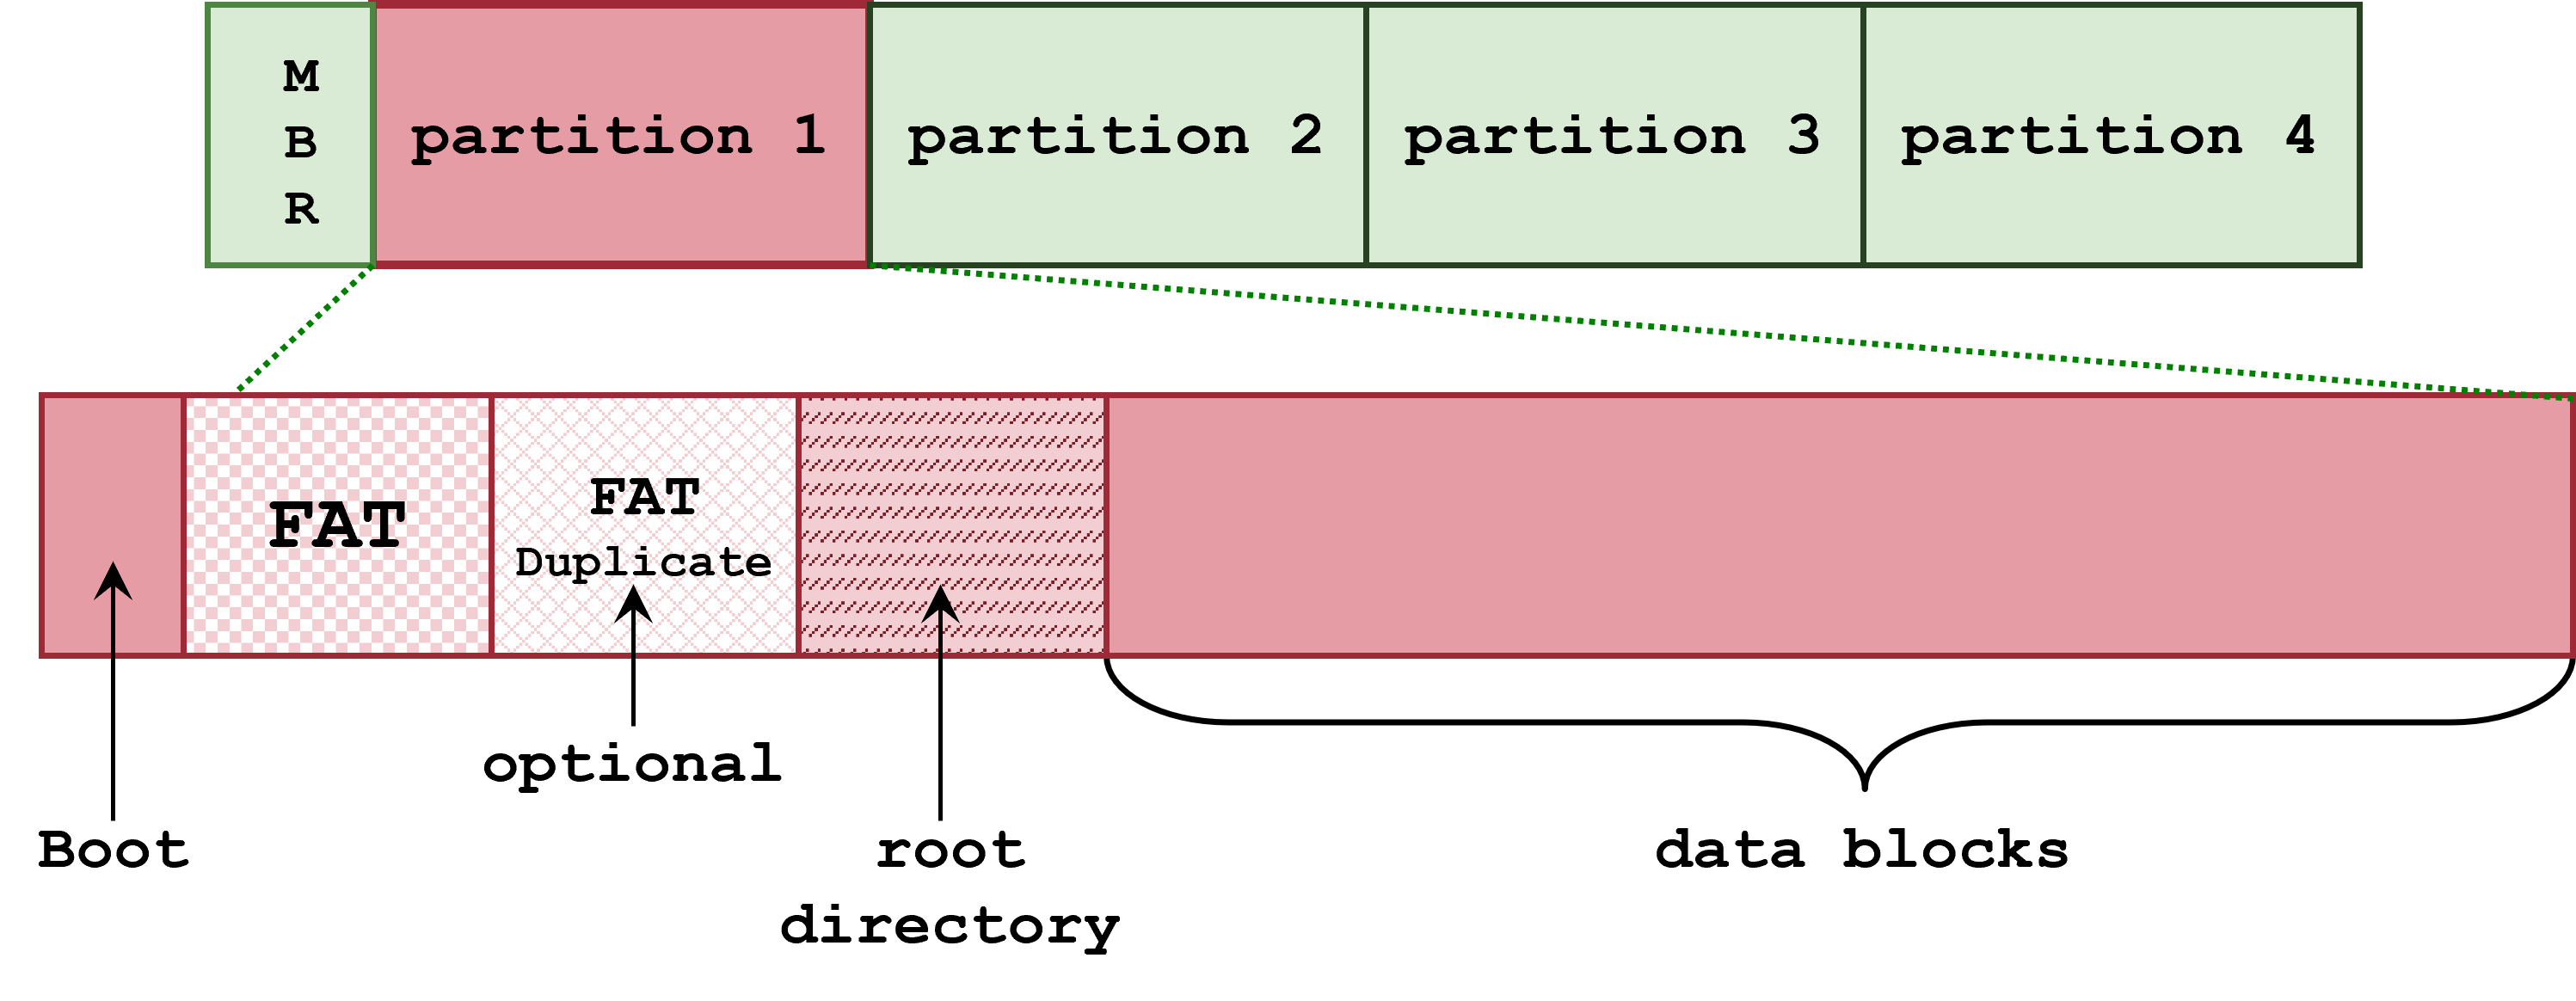
\includegraphics[width=8.5cm, height=2.3cm]{images/microsoftfat.png}

% 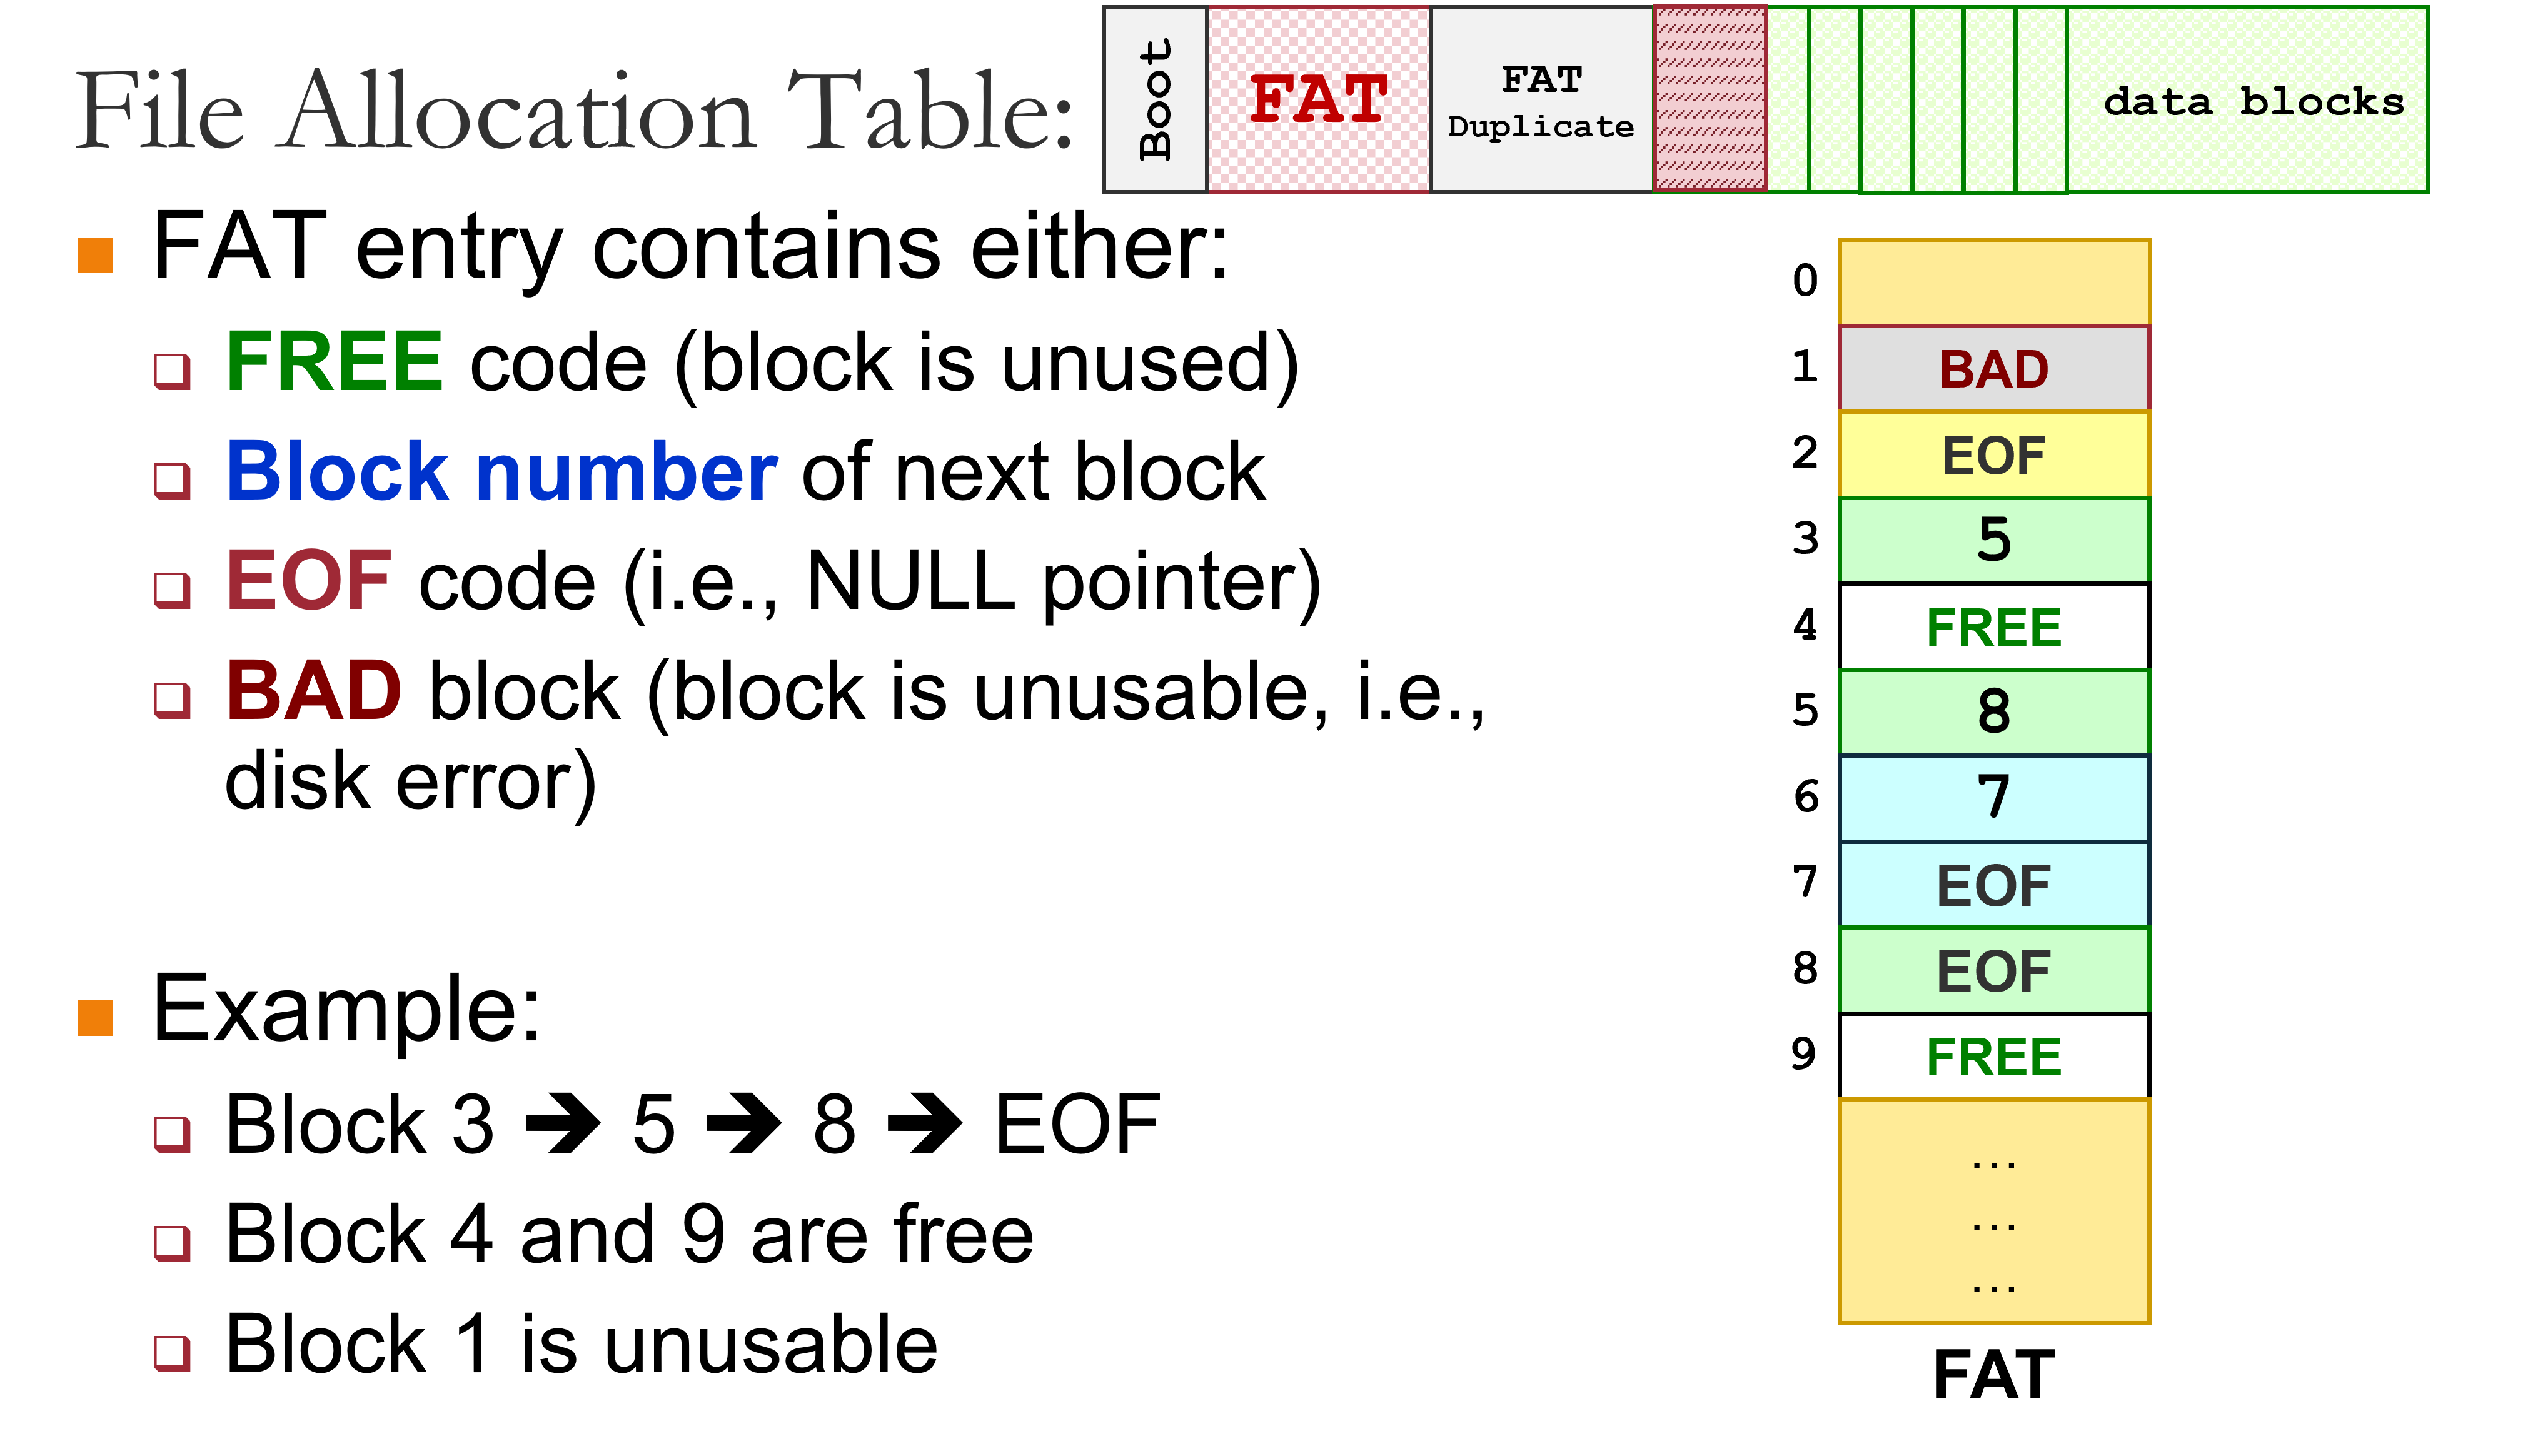
\includegraphics[width=8.5cm, height=3.8cm]{images/fatallocationtable.png}

\subsubsection*{Directory Structure and File Info}
\begin{itemize}[topsep=0pt,noitemsep,wide=0pt, leftmargin=\dimexpr\labelwidth + 2\labelsep\relax]
    \item Folder represented as special type of file. Root directory stored in special location (others stored in data blocks.)
    \item File/subdirectory in a folder represented as 1 directory entry.
    \item \textbf{Directory Entry} are fixed size 32-bytes. Contains: Name + Ext, Attributes (RDONLY, Dir/File flag, Hidden etc), Creation Date + time, First disk block + File size.
\end{itemize}

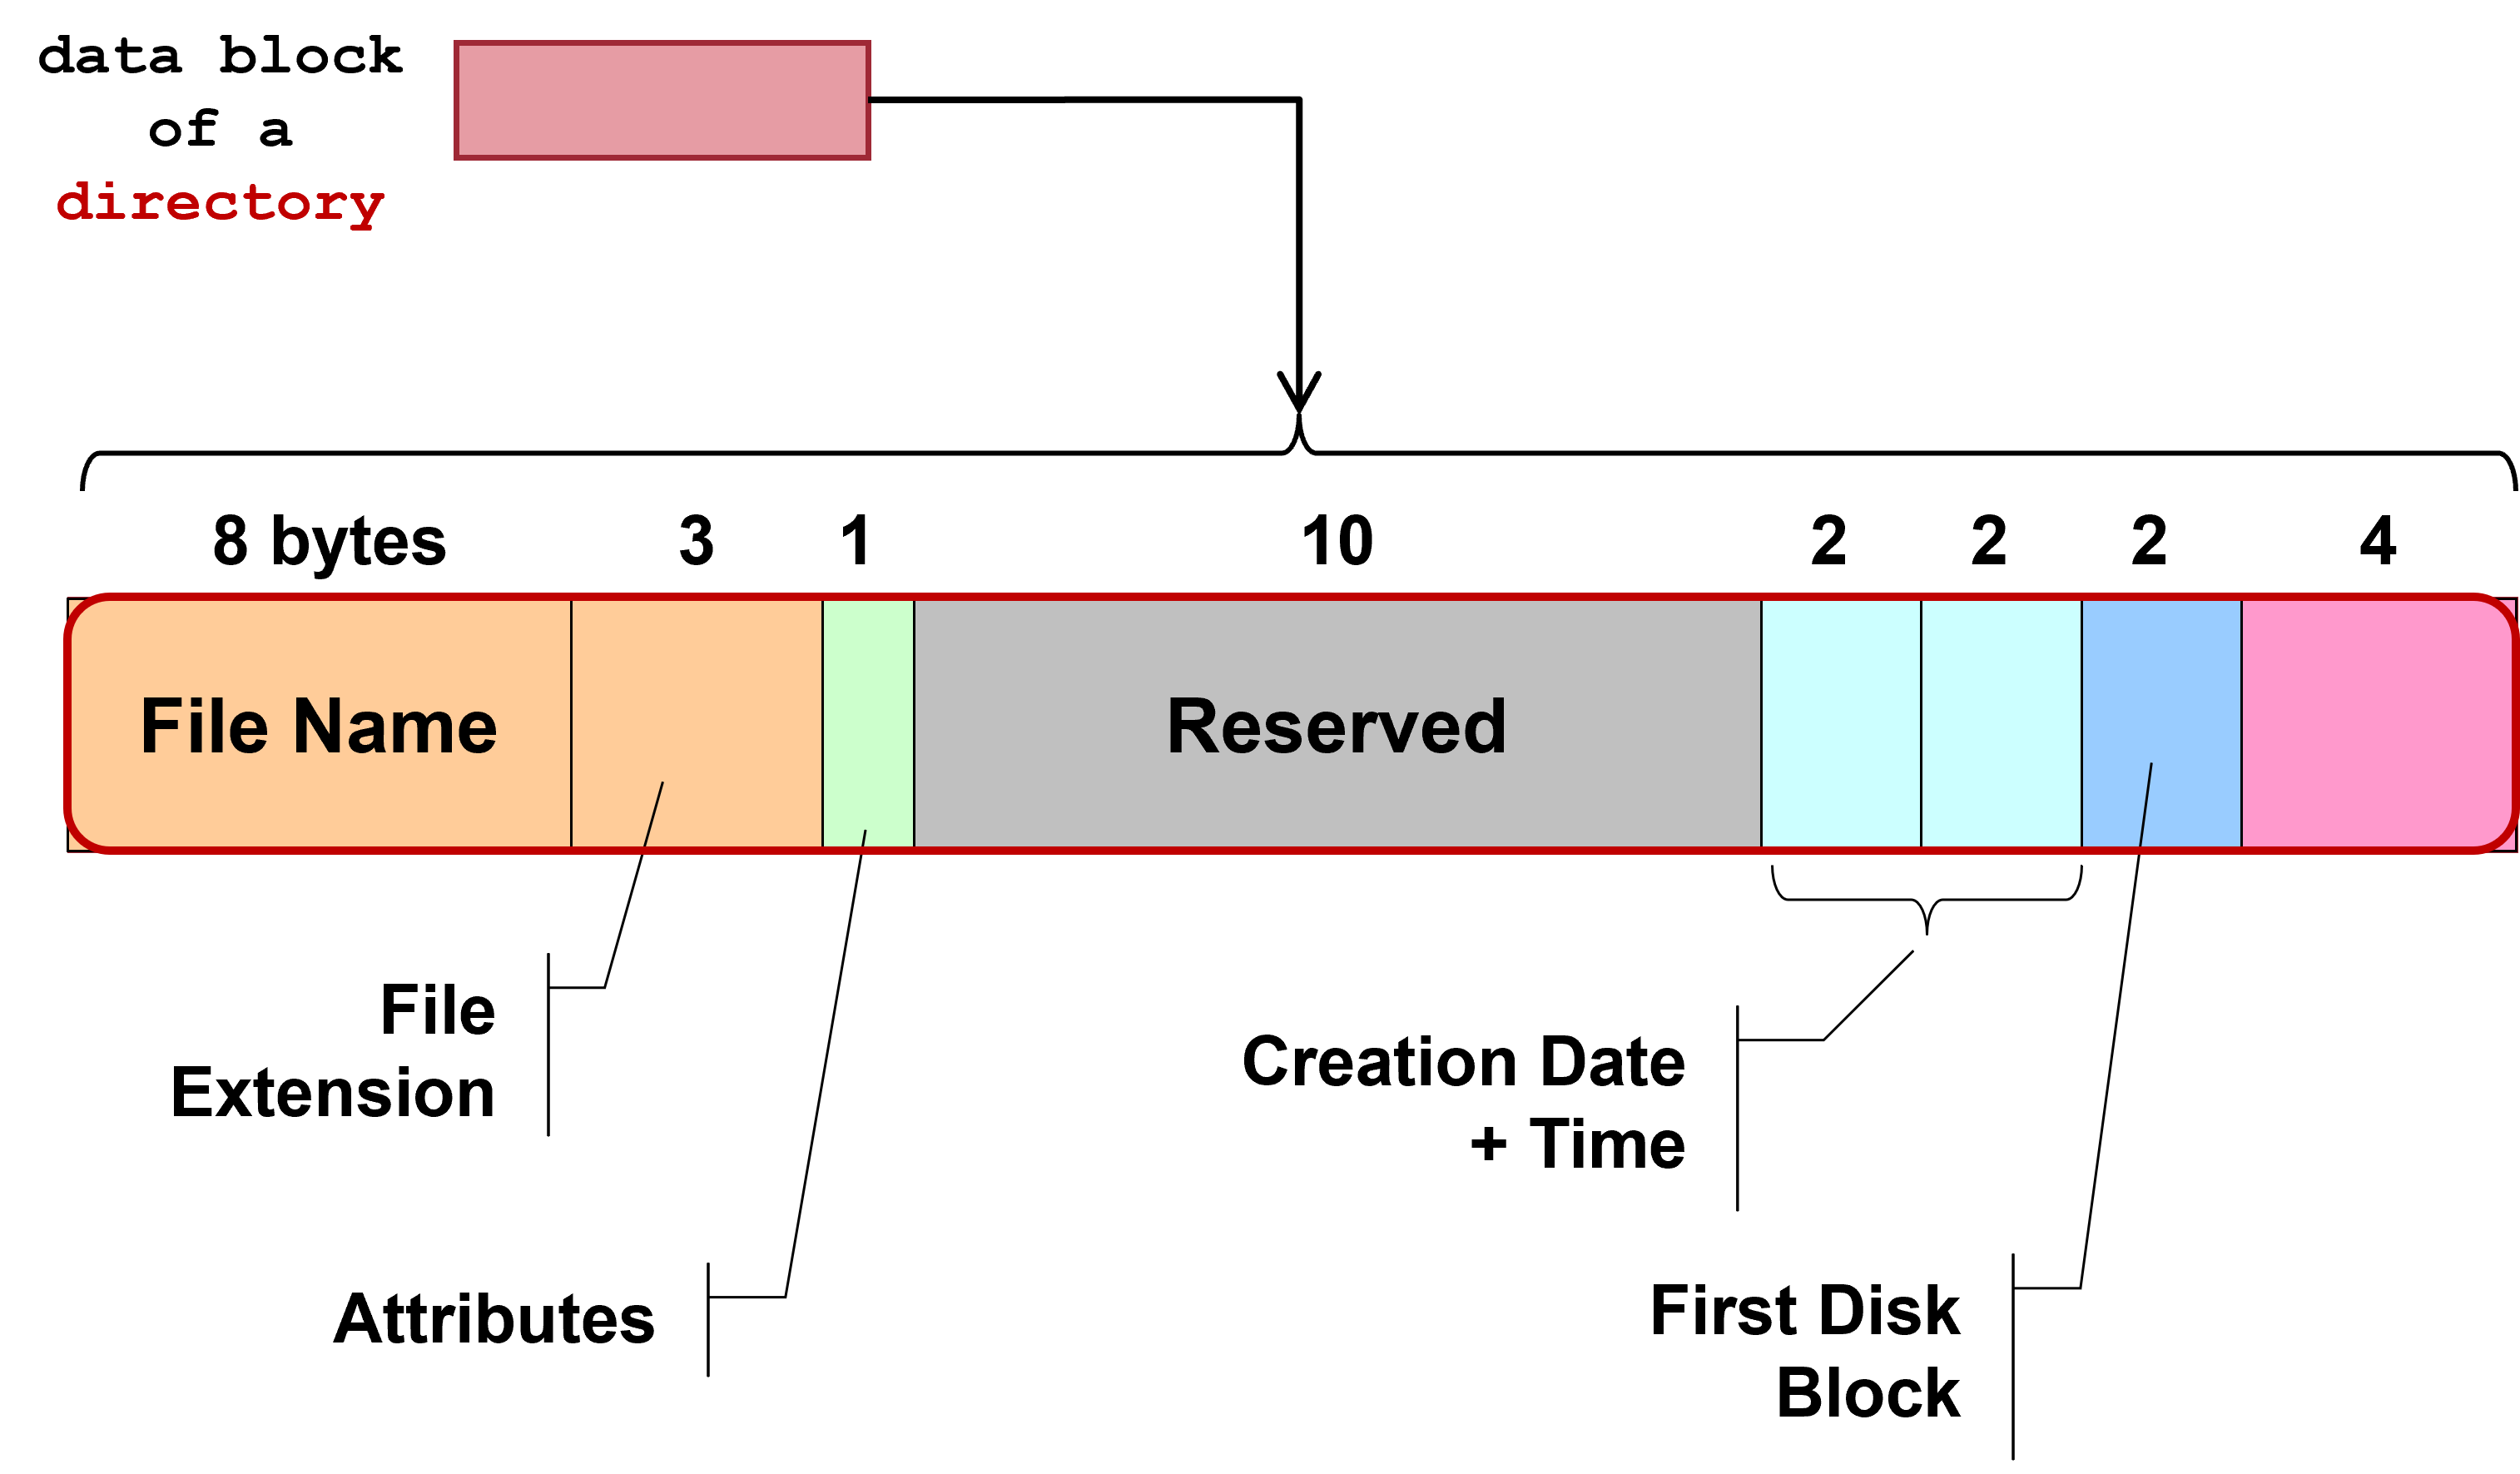
\includegraphics[width=4.2cm, height=2.5cm]{images/fatdirectory.png}
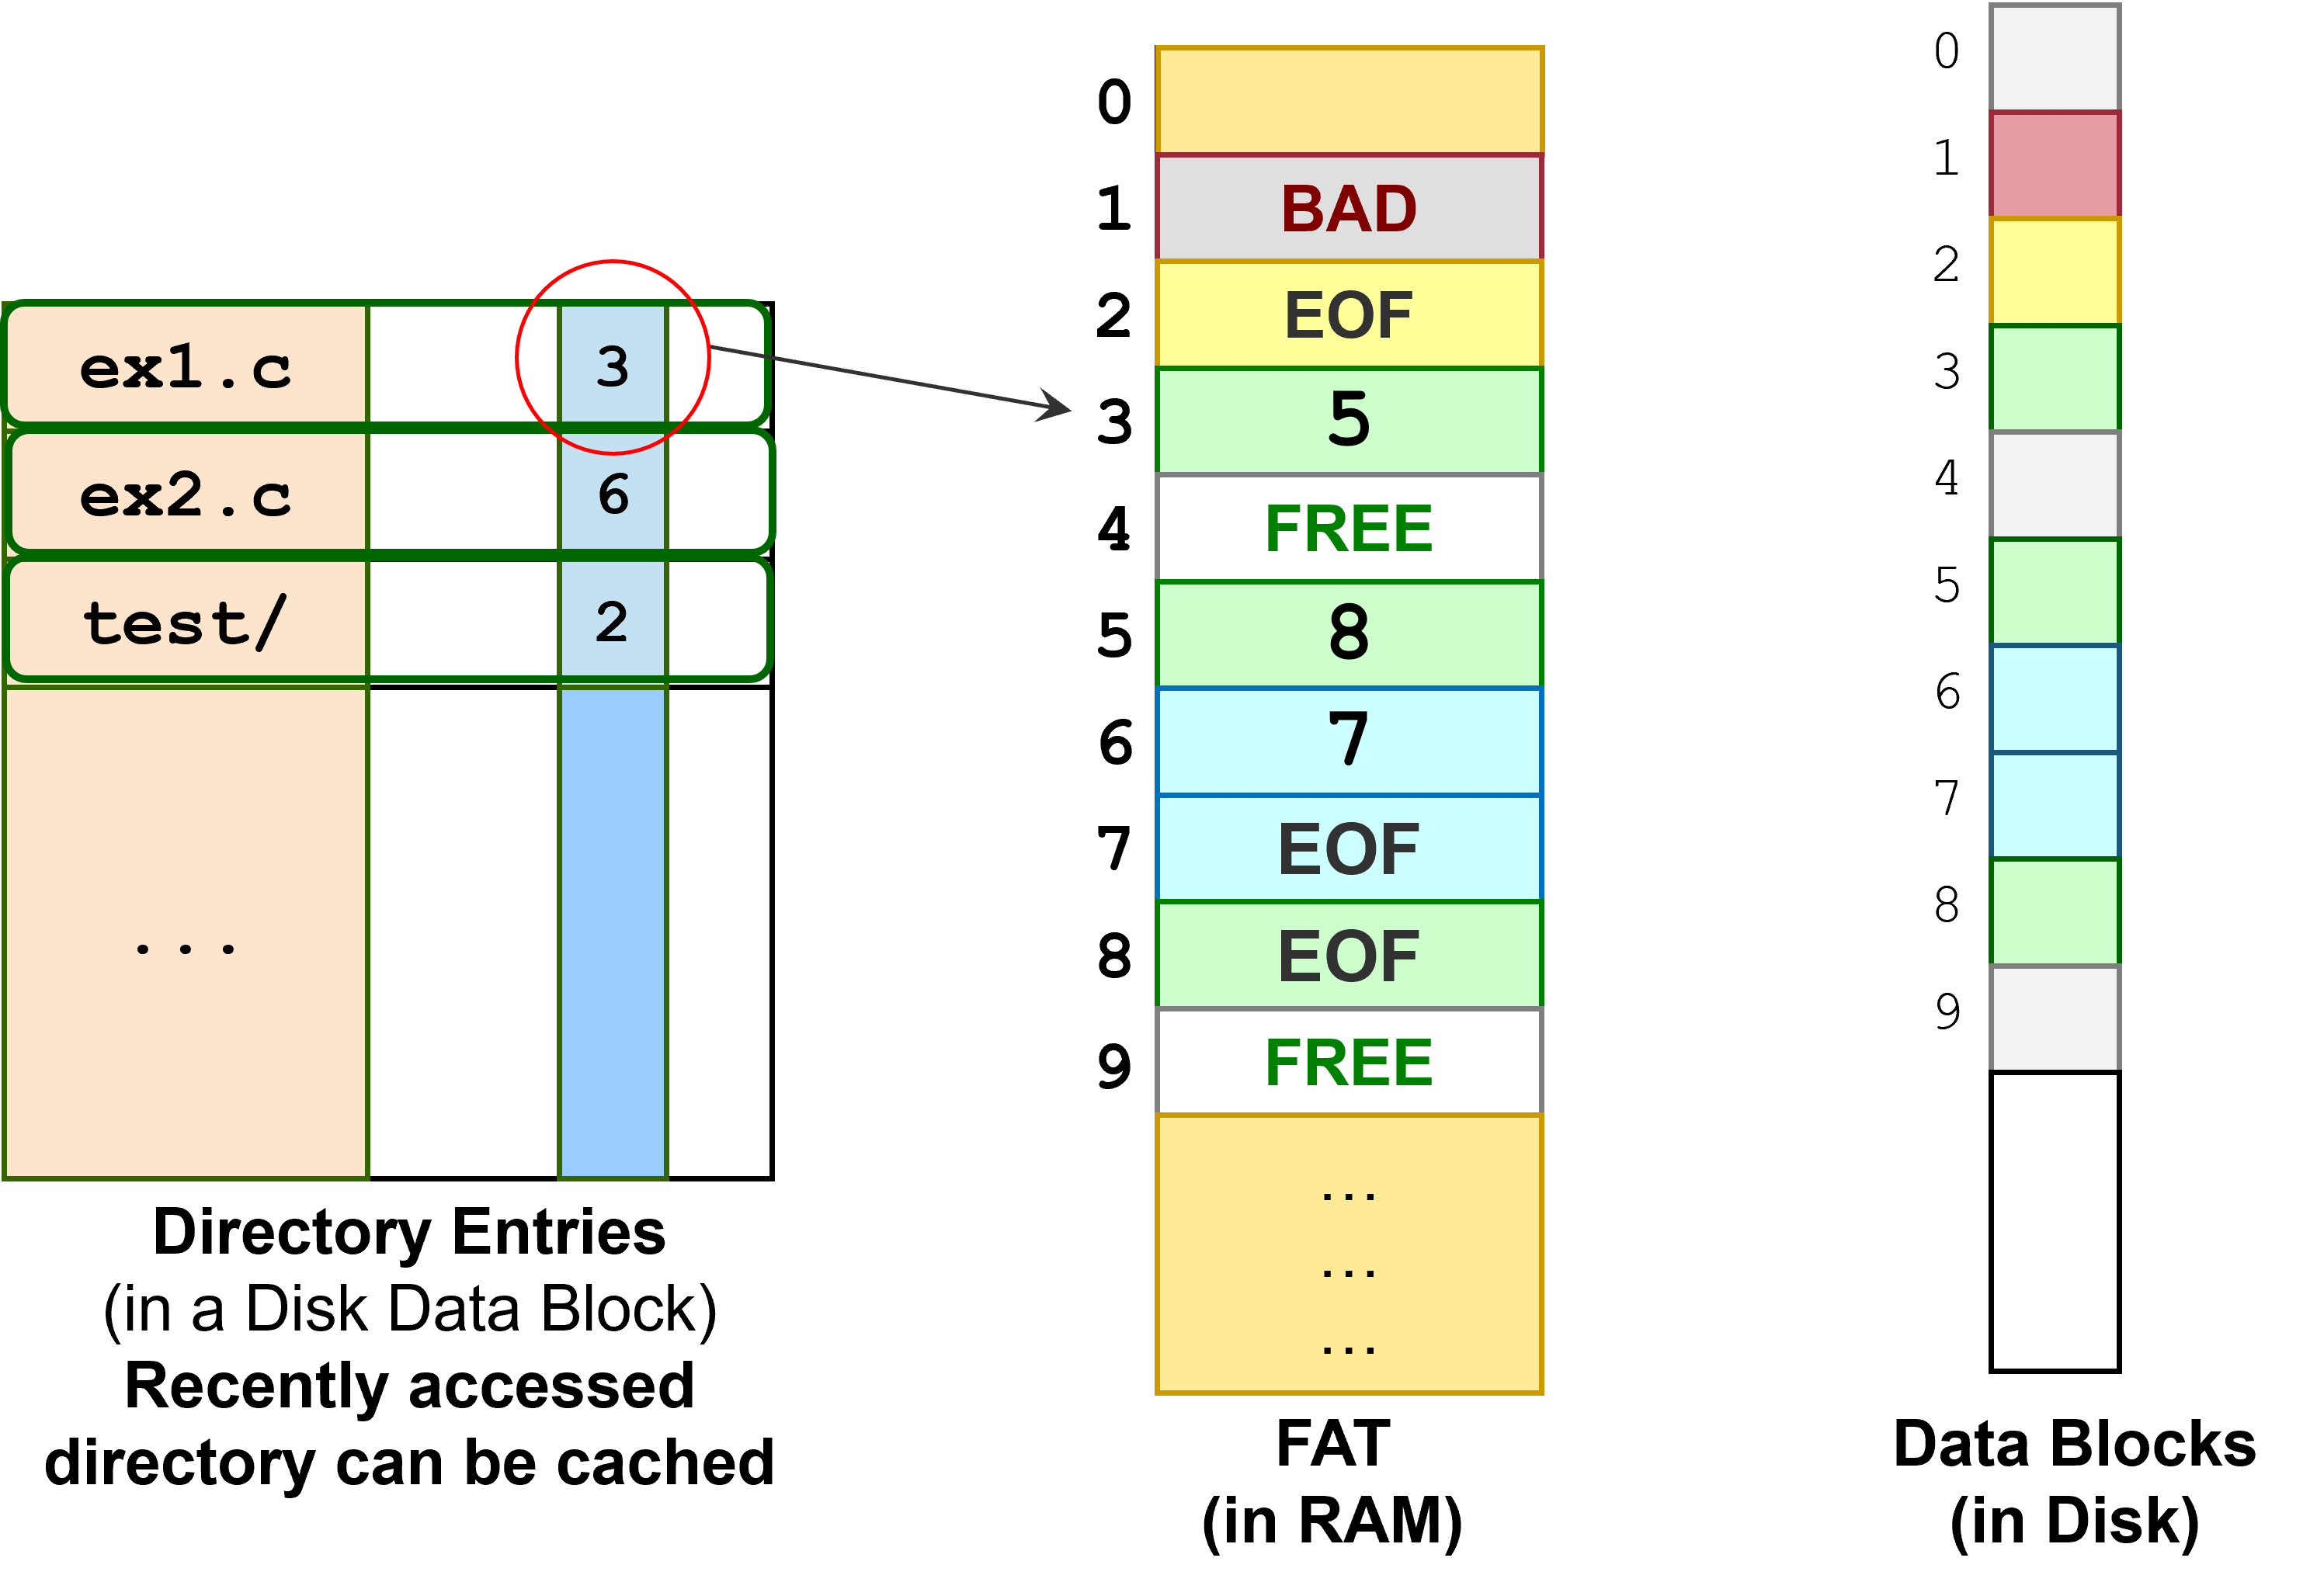
\includegraphics[width=4.2cm, height=2.5cm]{images/fatfs.png}

\subsubsection*{Directory Entry Fields}
\begin{itemize}[topsep=0pt,noitemsep,wide=0pt, leftmargin=\dimexpr\labelwidth + 2\labelsep\relax]
    \item \textbf{File Name + Extension:} Limit to 8+3 chars. First byte of file name may mean: deleted, end of dir entries, parent dir etc.
    \item \textbf{File Creation Time and Date:} Year limtied to 1980 to 2107, accuracy of seconds +- 2s
    \item \textbf{First Disk Block Index:} Different variants use different number of bits, FAT32 = 32bits
\end{itemize}


\subsection*{Extended-2 File System | Linux}
Disk space split into \textbf{Blocks}, grouped into \textbf{Block Groups}.
Each File/Dir is described by an \textbf{I-Node}, containing File metadata (access right, creation time etc.) and Data block addresses.

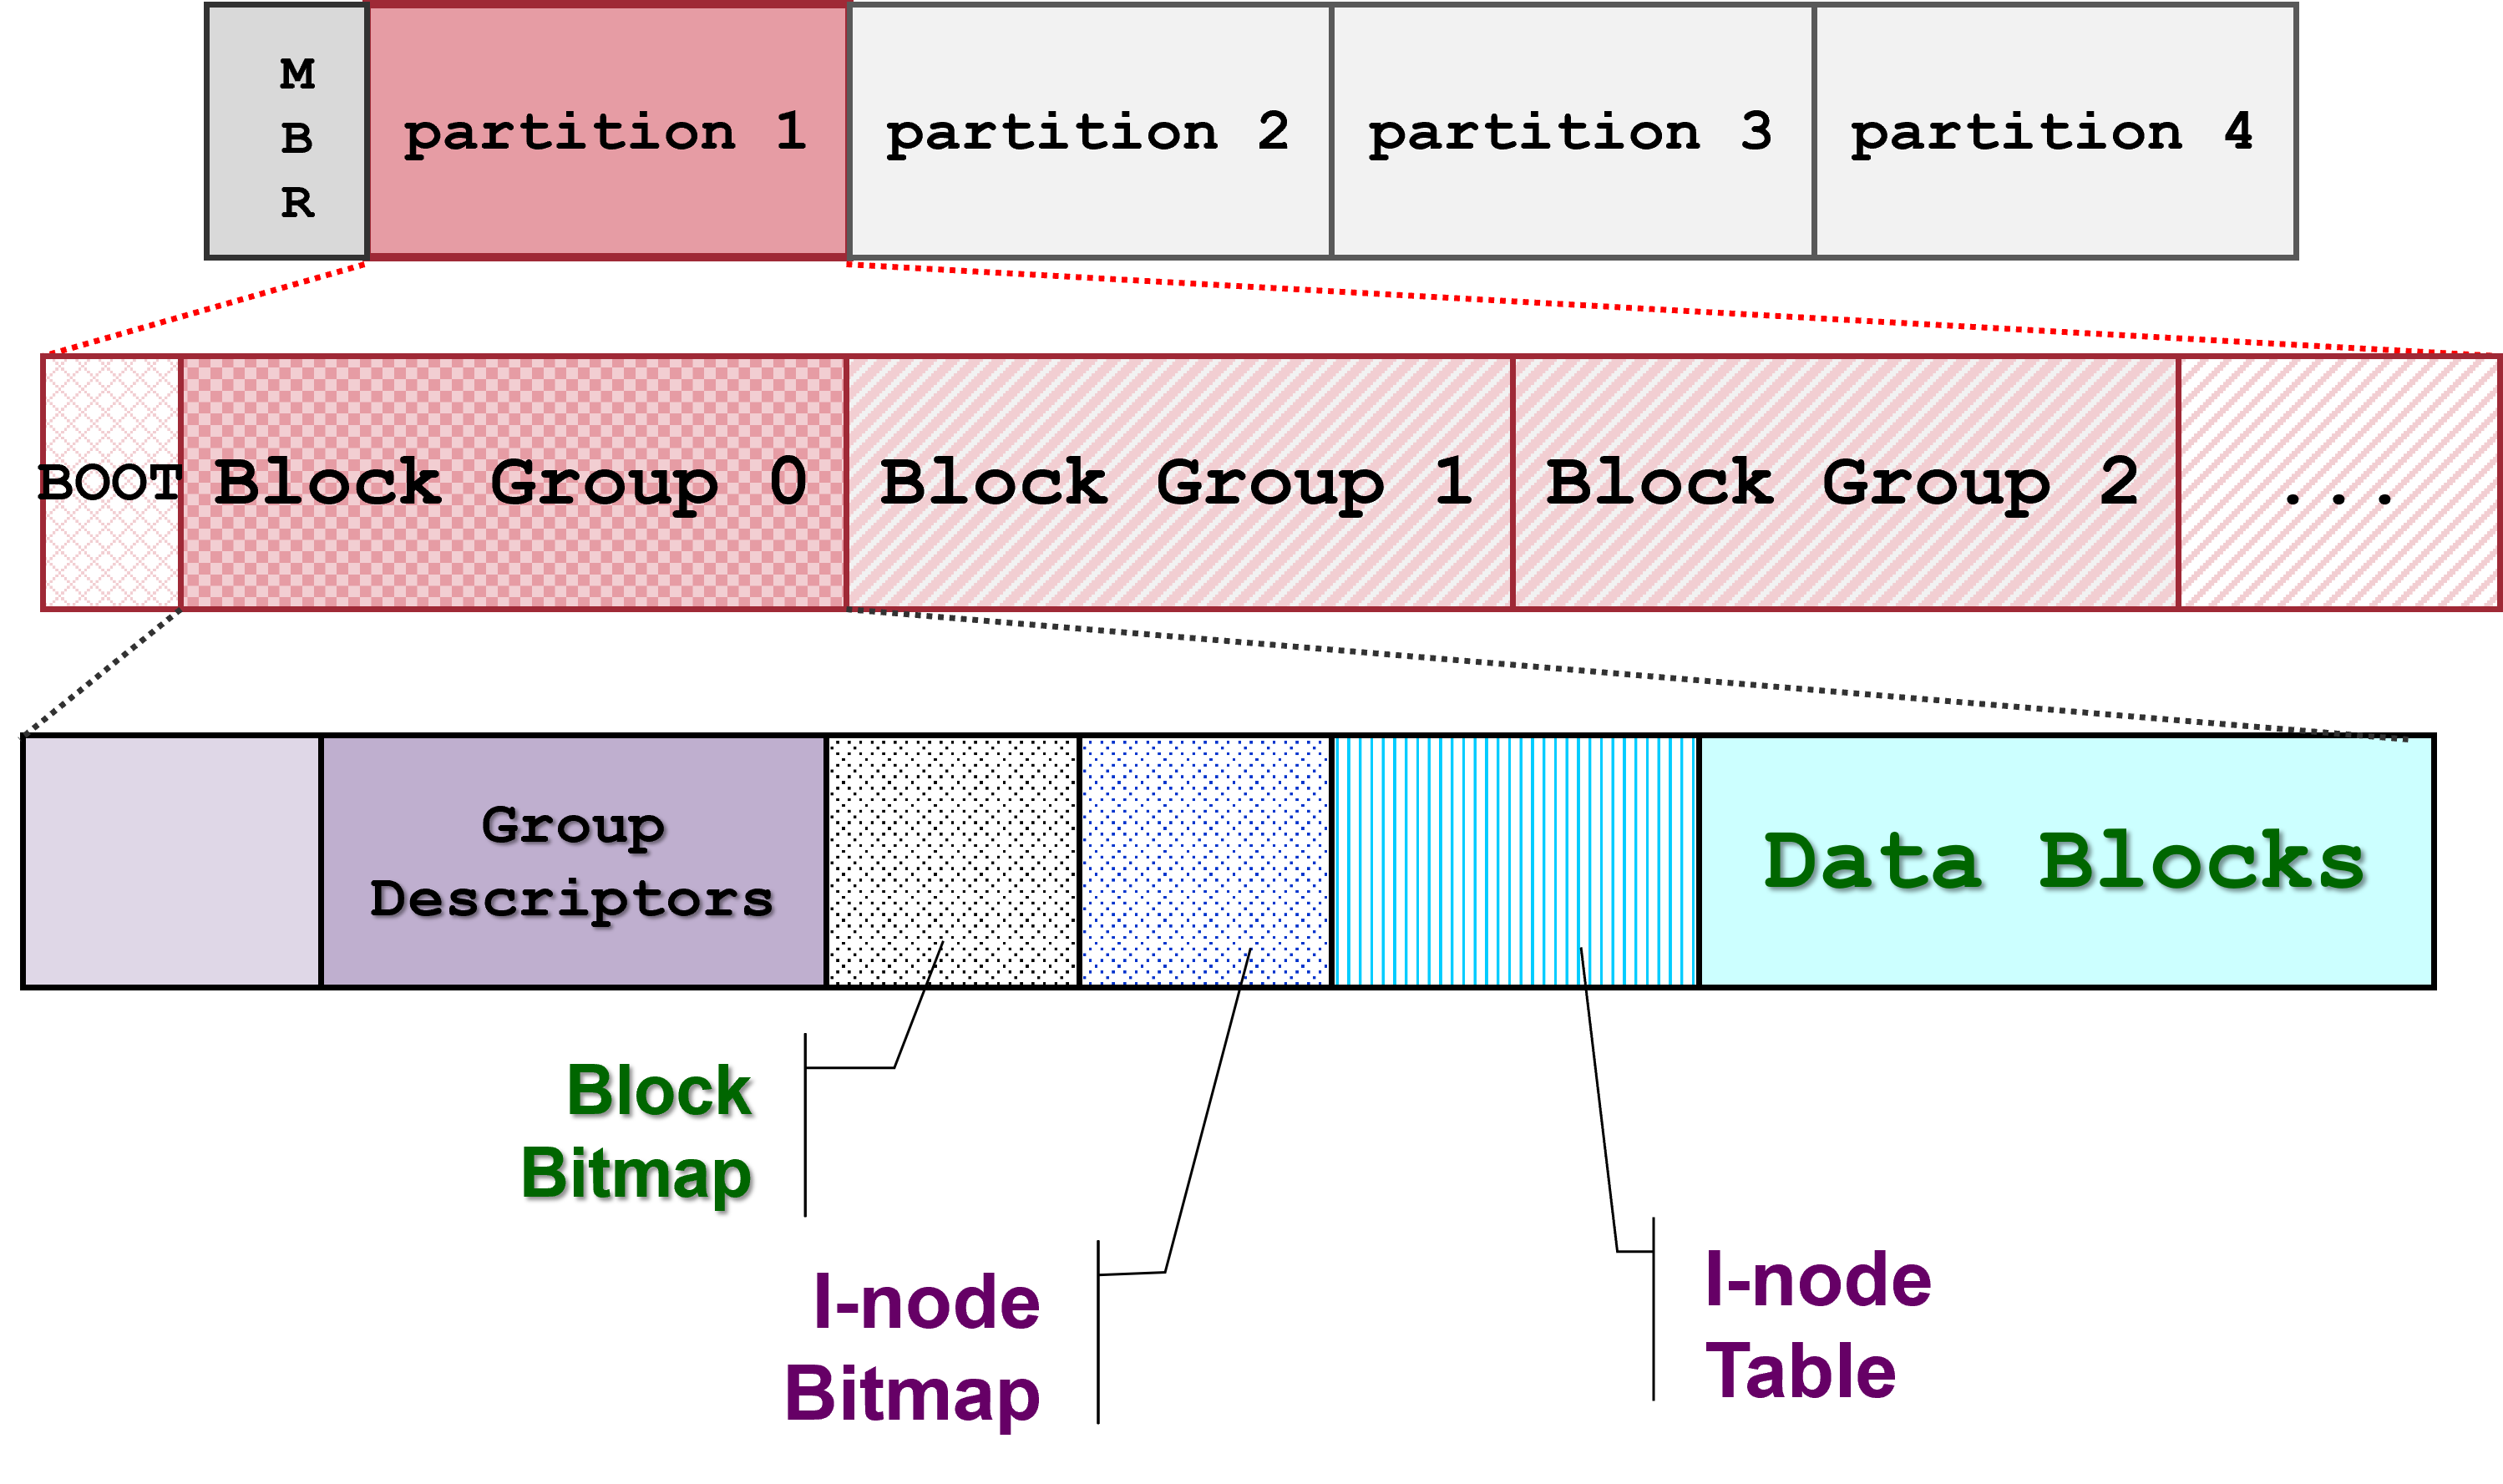
\includegraphics[width=8.5cm, height=3cm]{images/ext2layout.png}

\subsubsection*{Partition Information}
\begin{itemize}[topsep=0pt,noitemsep,wide=0pt, leftmargin=\dimexpr\labelwidth + 2\labelsep\relax]
    \item \textbf{Super Block:} Describes whole FS: Total I-Node number, I-Node per group. Total disk blocks, disk blocks per group.
    \item \textbf{Group Descriptors:} Describe each of the group, number of free disk blocks, free I-Nodes, location of bitmaps. Duplicated in each block group as well.
    \item \textbf{Block Bitmap:} Track usage of status of blocks in block group (1=Occupied, 0=Free)
    \item \textbf{I-Node Bitmap:} Track usage of status of I-Nodes in block gorup
    \item \textbf{I-Node Table:} Array of I-Nodes, each I-Node access by its index, contains only I-nodes of this block group
\end{itemize}

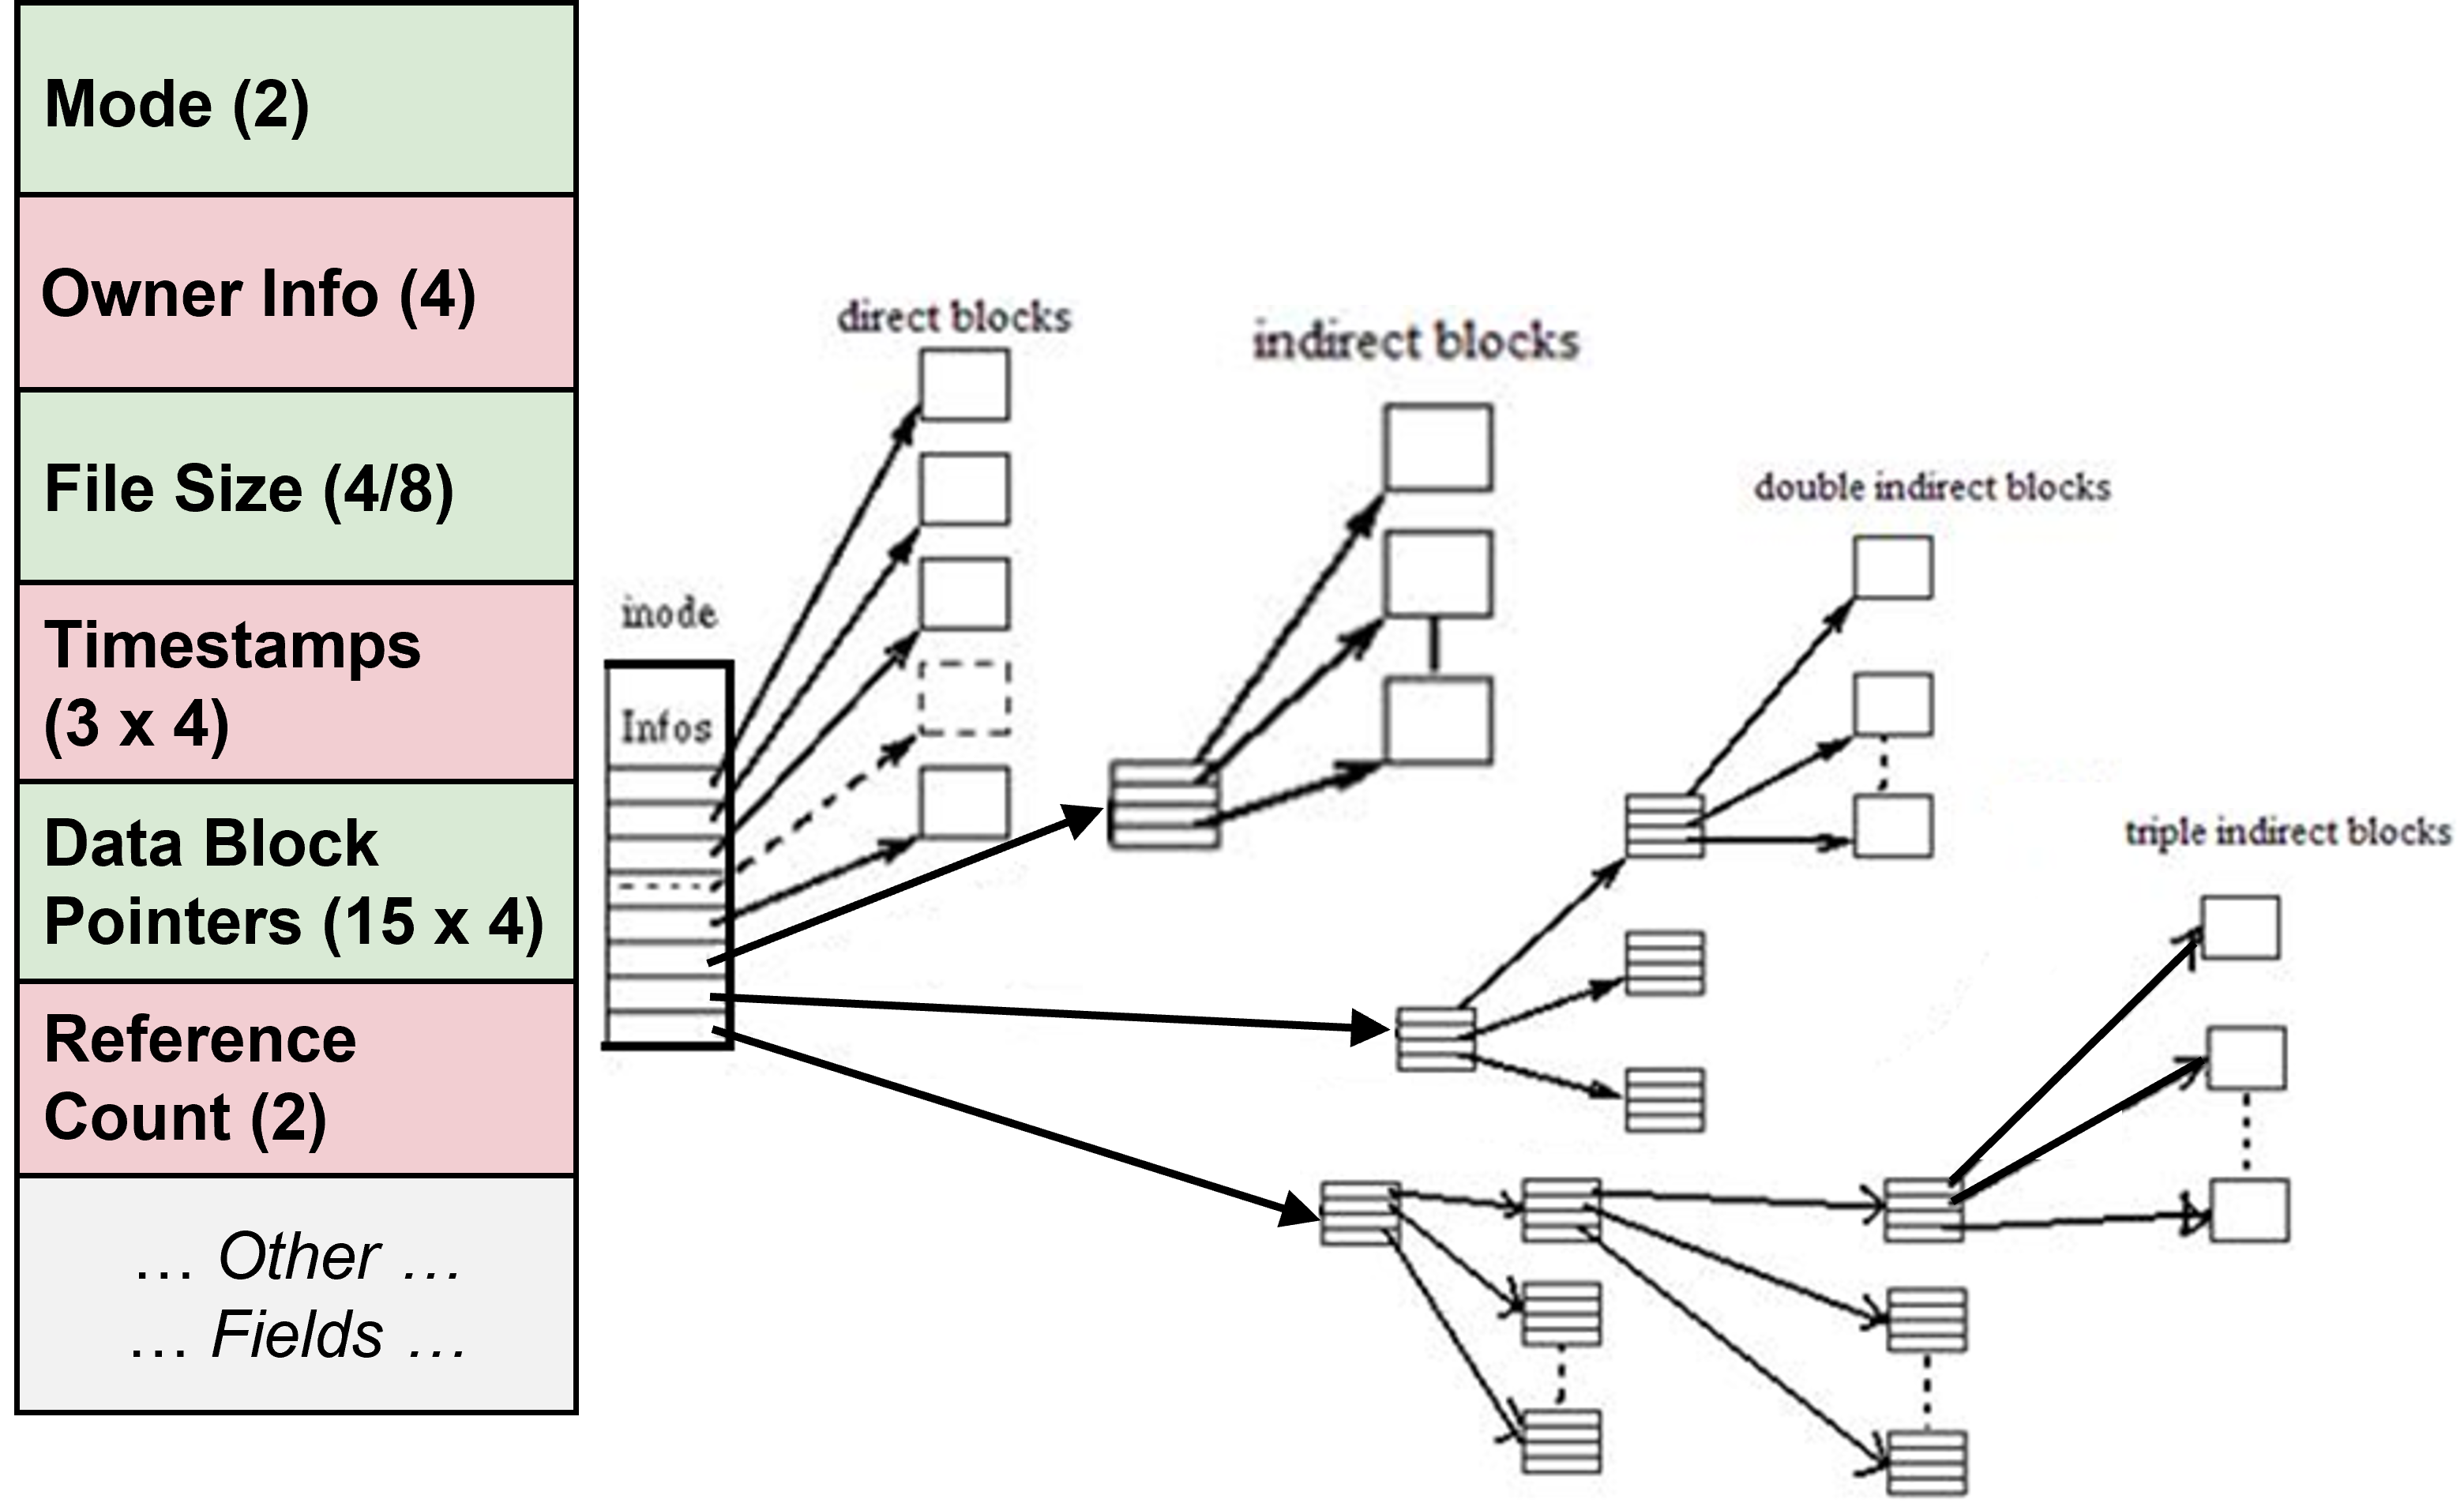
\includegraphics[width=7.5cm, height=3cm]{images/inodestructure.png}
\subsubsection*{I-Node Data Blocks}
15 Disk block pointers, first 12 pointers are \textbf{Direct Blocks}, 13$^{th}$ \textbf{Single Indirect}, 14$^{th}$ \textbf{Double Indirect}, 15$^{th}$ \textbf{Triple Indirect}. 
Direct blocks point directly to disk blocks, indirect blocks points to a block of pointers (also stored on data blocks).

\subsubsection*{Directory Structure}
Directory data blocks stores a \textbf{linked list of dir entries} for file / subdirectories information.
Each directory entry contains: 

\begin{multicols*}{2}
\begin{itemize}[topsep=0pt,noitemsep,wide=0pt, leftmargin=\dimexpr\labelwidth + 2\labelsep\relax]
    \item I-Node number for file/subdirectory
    \item Size of directory entry
    \item Length of file/subdirectory name
    \item Type: File or Subdirectory or Special File
    \item File/Subdirectory Name (255 chars max)
\end{itemize}
\end{multicols*}

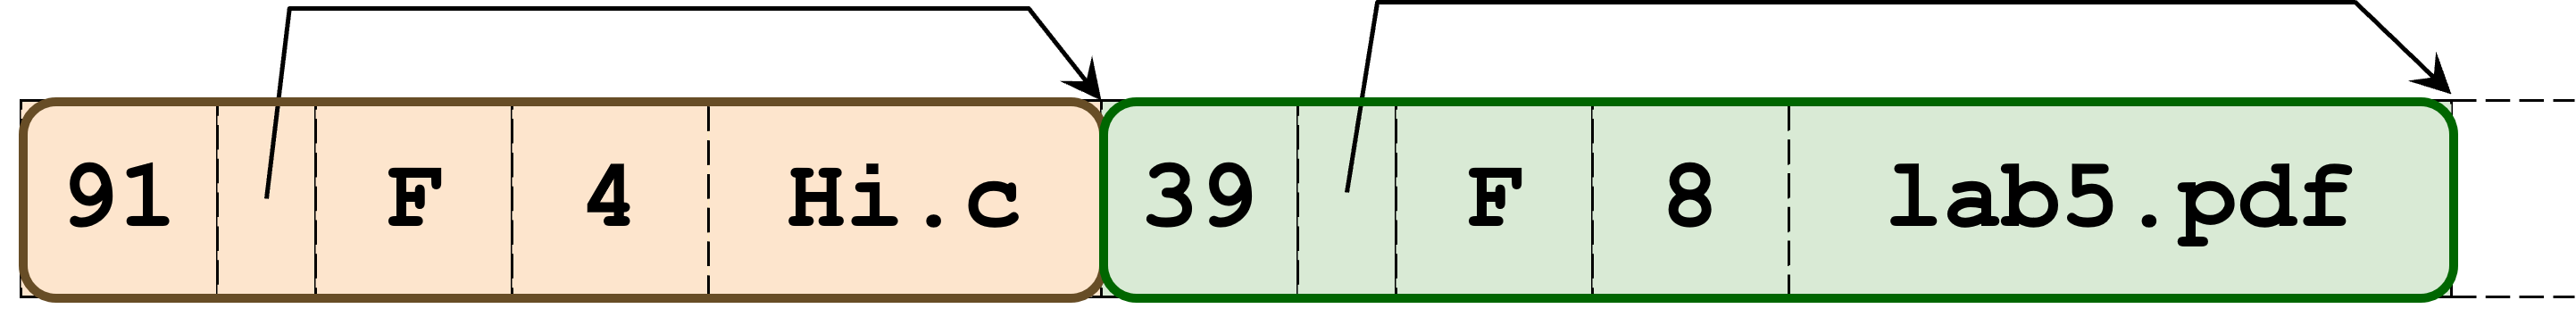
\includegraphics[width=8cm, height=0.7cm]{images/ext2dir.png}

\subsubsection*{Ext2: Hard vs Symbolic Link}
\begin{itemize}[topsep=0pt,noitemsep,wide=0pt, leftmargin=\dimexpr\labelwidth + 2\labelsep\relax]
    \item \textbf{Hard Link:} With multiple references of a I-Node, hard to determine when to delete an I-Node. Maintain I-Node reference count. decrement for every deletion.
    \item \textbf{Sym Link:} Only the pathname is stored, the link can be easily invalidated: File name changes / deletion etc.
    Involve a search to locate actual I-Node number of target file.
\end{itemize}

    
\subsubsection*{\underline{Tutorial + PYP Questions}}


% 1. \textbf{What is the max number of stack frames} \verb|facTail()| \textbf{function during the function call} \verb|facTail(5,1)| $\rightarrow$
% ft(5) $\rightarrow$ ft(4) $\rightarrow$ ... $\rightarrow$ ft(0), total of 6 stack frames maximum. \\

% \noindent 2. \textbf{Briefly describe how we can exploit the behavior of tail‐recursive function call to reduce the usage of 
% stack memory.} $\rightarrow$ Stack frame for a function only needs to be maintained if it is 
% going to continue execution. In tail recursion, once a function make a recursive call, 
% it ceased to be useful. So, the best way to exploit tail recursion is to overwrite the current 
% stack frame instead of allocating a new frame. In total, for the entire function, we only need \verb|1| stack frame.

\textbf{pthread Mutex and Conditional Variables}
\begin{itemize}[topsep=0pt,noitemsep,wide=0pt, leftmargin=\dimexpr\labelwidth + 2\labelsep\relax]
    \item Synchronisation mechanism for \verb|pthreads|
    \item Mutex (\verb|pthread_mutex|)
    \begin{itemize}[topsep=0pt,noitemsep,wide=0pt, leftmargin=\dimexpr\labelwidth + 2\labelsep\relax]
        \item Binary semaphore (i.e. equivalent Semaphore(1))
        \item Lock: \verb|pthread_mutex_lock()|
        \item Unlock: \verb|pthread_mutex_unlock()|
    \end{itemize}
    \item Conditional Variables (\verb|pthread_cond|)
    \begin{itemize}[topsep=0pt,noitemsep,wide=0pt, leftmargin=\dimexpr\labelwidth + 2\labelsep\relax]
        \item Wait: \verb|pthread_cond_wait()|
        \item Signal: \verb|pthread_cond_signal()|
        \item Broadcast: \verb|pthread_cond_broadcast()|
    \end{itemize}
    \item \textbf{Semaphore vs POSIX thread condition variable signal:}
    Semaphore signal increments count and may wake a waiting thread. If there is no thread
    sleeping on semaphore, it allows next thread requesting a “down” to proceed without
    blocking. A conditional signal has no concept of count. It wakes up one thread currently sleeping on
the condition, has no (lasting) impact on later threads that may be waiting on condition.
\end{itemize}

\textbf{Context Switching}
\begin{itemize}[topsep=0pt,noitemsep,wide=0pt, leftmargin=\dimexpr\labelwidth + 2\labelsep\relax]
    \item Involve process transitioning from READY state to RUNNING state, other process \textbf{being switched out} of is still in the RUNNING state.
    \item Before switching, current PC should be saved in the PCB to restore process execution when process gets CPU back.
    \item Context switching can still occur even if interrupts are disabled -- though a context switch can occur \underline{as a result of} an interrupt.
\end{itemize}

\textbf{Critical Section || Ordering of Mutex} \\ 
\textbf{Suppose a critical section requires M mutex locks before it can be executed.
Show why if every process acquires the locks in the same order, then a deadlock
cannot occur. Would it also matter if the processes \textit{unlock} the mutex lock in different orders?}

\begin{itemize}[topsep=0pt,noitemsep,wide=0pt, leftmargin=\dimexpr\labelwidth + 2\labelsep\relax]
    \item Suppose the M locks are labelled L$_1$ to L$_M$. All threads competing for the locks in the same
    order ensures that L$_1$ in effect acts like the lock for L$_2$ to L$_M$ as well as the critical section.
    There can be no deadlock because no other thread can acquire any of L$_2$ to L$_M$ without first
    contending for L$_1$.
    \item Doesn’t matter because the locks has to be acquired in the same order. Even if another thread
    release lock L$_i$ first before L$_1$, until it releases L$_1$, no other thread can proceed beyond L$_1$. 
\end{itemize} 
\includegraphics*[width=7.6cm, height=3cm]{images/ititimequantum.png}

\textbf{MLFQ Task Scheduling:}
Suppose there are three priority queues, Q0, Q1, and Q2 with Q0 having the
lowest and Q2 having the highest priority. Now suppose there are 2 tasks, both
present at the start. Task A is I/O bound, it will run for 1 time unit on the CPU before
blocking for I/O for 5 time units. This is repeatedly 9 times before 1 final 1 time unit
CPU execution to finish off the task. Task B is CPU bound and will run for 200 time
units. Assuming that the time quantum is set at 10 time unit and that the OS takes no
overhead, show the schedule under Multi-level Feedback Queue for 200 time units
with Task A starting the schedule. For simplicity, we assume that the queues are never
reset.
\includegraphics*[width=7.6cm, height=3cm]{images/mlfqscheduling.png}

\textbf{File Descriptors:}
A process has 3 threads, T1, T2, and T3, and its code does not contain any \verb|exec*()|
commands. T1 opens 3 files and T2 creates a pipe. After these actions, T1 executes a
\verb|fork()| command and T2 executes a \verb|fork()| whose child immediately calls \verb|execvp()| to
execute a single-threaded program. T1 closes the three files and then terminates. T3
terminates without opening any file. Note that all threads are POSIX threads.

\framebox{\parbox{\dimexpr\linewidth-2\fboxsep-2\fboxrule}{% 
    $\star$ On a Unix-like operating system, the first three file descriptors, by default, are STDIN, STDOUT and STDERR.
    T1 creates 3 fds, T2 creates 2 fds. There are 8 fds in the process now. After this, there are 2 fork() calls $\rightarrow$ 
    each process will duplicate the fd table with 8 fds: 24 fds are created in total.

    \begin{itemize}[topsep=0pt,noitemsep,wide=0pt, leftmargin=\dimexpr\labelwidth + 2\labelsep\relax]
        \item If threads read from same fd, they would read different content, since offset is shared in the system-wide open file table.
        \item Suppose each thread opens file indepedently, fd is different, thus content read is the same, as both reads the entire file.
    \end{itemize}
}}

\textbf{Virtual Memory Address vs Virtual Address Space:}
$32$ bit virtual \textit{memory addresses}, and question 5 mentions $2^{64}$ bit \textit{address space}. Each address points to $1$ byte in memory, so $32$ bit memory address will be able to represent $2^{32}$ bytes. Therefore the \textit{address space} is $2^{32}$ bytes or $2^{35}$ bits. 
However, $2^{64}$ bit address space is the total amount of data \textit{memory addresses} point to, and hence we have to convert to bytes, as $2^{64}$ bit address space doesn't mean $64$ bits are used for addressing.

\textbf{Single-Core Architectures:}
Every instruction on a single-core machine is effectively atomic, including the ordinary increment instruction on S1.  Therefore, for S1, as long as the entire critical section fits in one instruction, which is the case here, there is no way to violate mutual exclusion. In all other cases, mutual exclusion is not guaranteed and race conditions are possible.

\textbf{Page Replacement Algo:} Given 5 physical frames for a process. After the following sequence of page accesses(memory reference
string), what are the pages in RAM sorted from first frame to last frame?
\underline{Sequence: 3, 2, 4, 5, 1, 5, 7, 4, 7, 6, 3, 5}
\begin{enumerate}[topsep=0pt,noitemsep,wide=0pt, leftmargin=\dimexpr\labelwidth + 2\labelsep\relax]
    \item \textbf{LRU:} 7, 6, 4, 5, 3 $\rightarrow$ \sout{3} 7, \sout{2} 6, 4, 5, \sout{1} 3 
    \item \textbf{FIFO:} 7, 6, 3, 5, 1 $\rightarrow$ \sout{3} 7, \sout{2} 6, \sout{4} 3, 5, 1
    \begin{lstlisting}
clock_algo(incoming_page):
    if (present_in_frame(incoming_page)): 
        update same_page_in_frame.bit to 1
        clock_algo(receive_next_page)
    else: // incoming page not present in frame
        if (victim_pointer.page.bit == 1): 
            victim_pointer.page.bit = 0
            victim_pointer = next_page_in_frame
            clock_algo(incoming_page) // REDO PAGE
        else: // MOVE ON TO NEXT PAGE
            swap(victim_pointer.page)
            victim_pointer = next_page_in_frame
            clock_algo(receive_next_page) 
    \end{lstlisting}
\end{enumerate}

% \includegraphics*[width=8.6cm, height=9cm]{images/Tutorial1.png}
% \includegraphics*[width=8.6cm, height=4.5cm]{images/Tutorial3a.png}
% \includegraphics*[width=8.6cm, height=3cm]{images/Tutorial3c.png}
% \includegraphics*[width=8.6cm, height=3.5cm]{images/Tutorial3b.png}
% \includegraphics*[width=8.6cm, height=6cm]{images/Tutorial3d.png}
% \includegraphics*[width=8.6cm, height=9.5cm]{images/Tutorial4.png}
% \includegraphics*[width=8.6cm, height=6.2cm]{images/Tutorial5a.png}
% \includegraphics*[width=8.6cm, height=7.2cm]{images/Tutorial5b.png}
% \includegraphics*[width=8.6cm, height=2.5cm]{images/factorialrecursive.png}

\end{multicols*}

\end{document}